%
% ---------------------------------------------------------------------------------------
% 2010 / 1.431E+20 POT Muon-Neutrino Disappearance Analysis 
% ---------------------------------------------------------------------------------------
%

\documentclass[final]{elsarticle}

\usepackage[margin=2.00cm]{geometry}  % tweak margins
%\usepackage{draftcopy}                % uncomment to print a "DRAFT-COPY" in background
\usepackage{graphicx}                 % if you want to include PostScript figures
\usepackage[figuresright]{rotating}   % if you have landscape tables
\usepackage{multirow}                 % fancy tables
\usepackage[toc,page]{appendix}       % appendix
\usepackage{lineno}                   % for printing the line numbers
\usepackage{natbib}                   % for building bibliography with \cite{}
\usepackage{setspace}
\usepackage{times}
\usepackage{afterpage}
\usepackage{float}
\usepackage{subfigure}
\usepackage{color} 

% use to fix date
% \def \today { February 1st, 2009 }
% put your own definitions here:
\newcommand{\ttbs}{\char'134}
\newcommand{\AmS}{{\protect\the\textfont2
  A\kern-.1667em\lower.5ex\hbox{M}\kern-.125emS}}
% add words to TeX's hyphenation exception list
\hyphenation{author another created financial paper re-commend-ed Post-Script}

%\linenumbers
\bibliographystyle{elsart-num}

% By default, LaTeX doesn't like to fill more than 0.7 of a text page with tables and graphics, 
% nor does it like too many figures per page. Change this behaviour:
\renewcommand\floatpagefraction{.95}
\renewcommand\topfraction{.9}
\renewcommand\bottomfraction{.9}
\renewcommand\textfraction{.1}   
\setcounter{totalnumber}{50}
\setcounter{topnumber}{50}
\setcounter{bottomnumber}{50}


\begin{document}

% Title, authors, abstract and table of contents
%
% Front matter
%

\begin{frontmatter}

\title{
  T2K 1.431$\times10^{20}$-POT Muon-Neutrino Disappearance Analysis
}

\vspace*{0.7cm}

\author[RAL]     {Costas Andreopoulos\corref{cor}}
\author[RAL,OXF] {Thomas Dealtry}
\author[ICL,RAL] {James Dobson}
\author[LANCS]   {Nick Grant}
\author[OXF]     {Martin Haigh}
\author[RAL]     {Jelena Ilic}
\author[RAL]     {Geoff Pearce}
\author[RAL,OXF] {and Alfons Weber}

\cortext[cor]{E-mail: costas.andreopoulos@stfc.ac.uk}

\address[RAL]{Particle Physics Dept., Rutherford Appleton Laboratory, STFC \\
              Harwell Science and Innovation Campus\\
              Oxfordshire OX11 0QX, UK}
\address[OXF]{Subdepartment of Particle Physics, University of Oxford \\
              Denys Wilkinson Building, Keble Road\\
              Oxfordshire OX1 3RH, UK}
\address[LANCS]{Physics Dept., Lancaster University \\
              Lancaster, LA1 4YB, UK}
\address[ICL]{Physics Dept., Imperial College London \\
              Blackett Lab, Prince Consort Road\\
              London SW7 2BW, UK}

%
% Abstract
%

\begin{abstract}

We report the results of a 2-flavour $\nu_{\mu}$-disappearance analysis on the combined Run1+2 dataset.
This combined dataset corresponds to an integrated JPARC neutrino beam
exposure of $1.431 \times 10^{20}$ POT.
The oscillation analysis was performed using both GENIE \cite{Genie:NIM} and NEUT \cite{Neut:ActaP}.
All of the inputs to the analysis are official 2010 inputs.

Using the ND280 measurement, GENIE predicts 101.72 $\pm$ 10.09 (stat) $^{+13.88}_{-13.49}$ (syst)
1 $\mu$-like ring events in SuperK without oscillations but only 31 were observed.
The statistical significance of the observed deficit is $\sim$4.2 standard deviations.
NEUT predicts 103.59 $\pm$ 10.18 (stat) $^{+13.77}_{-13.43}$ (syst) events in SuperK,
which implies that the statistical significance
of the observed deficit is $\sim$4.3 standard deviations.

The observed number of 1$\mu$-like ring events is consistent with 
the 2011 MINOS best-fit $\nu_{\mu}$-disappearance hypothesis
($sin^{2}2\theta_{23}$ = 1.0 and $|\Delta m^{2}_{23}|$ = 2.32$\times10^{-3}$ $eV^{2}/c^{4}$) \cite{Minos2011}.
Under this oscillation hypothesis,
GENIE predicts 28.39 $\pm$ 5.33 (stat) $^{+4.53}_{-4.46}$ (syst) 1 $\mu$-like ring events
in SuperK, while NEUT predicts 29.18 $\pm$ 5.40 (stat) $^{+4.31}_{-4.26}$ (syst) events. 

A 2-flavour $\nu_{\mu}$-disappearance fit to
the observed reconstructed energy spectrum of 1 $\mu$-like ring events of the combined Run1+2 dataset,
with $sin^{2}2\theta_{23}$ constrained to the physical region,
yields
$|\Delta m^{2}_{23}|$ = 2.60$\times$10$^{-3}$ $eV^{2}/c^{4}$ and
$sin^{2}2\theta_{23}$ = 0.97
as the best-fit values for GENIE ($\chi^{2}/ndf$ = 0.310).
For NEUT, the corresponding values are
$|\Delta m^{2}_{23}|$ = 2.65$\times$10$^{-3}$ $eV^{2}/c^{4}$ and
$sin^{2}2\theta_{23}$ = 0.98 ($\chi^{2}/ndf$ = 0.311).

\end{abstract}

%
% Keywords
%

%\begin{keyword}
%\end{keyword}

\end{frontmatter}

\clearpage

\tableofcontents

\clearpage

\listoffigures
\listoftables




% Main body
\clearpage

\section {Introduction }
\label{sec:intro}

In this technical note, 
we report the results of a 2-flavour $\nu_{\mu}$-disappearance analysis,
performed by the Rutherford-Oxford-Lancs groups,	
on the combined Run1+2 (1.431$\times$10$^{20}$ POT) dataset.
This dataset was collected in two run periods:
in January 2010 - June 2010 (Run1, 0.323$\times$10$^{20}$ POT) and
in November 2010 - March 2011 (Run2, 1.108$\times$10$^{20}$ POT).

This analysis 
\footnote{
   Preliminary results from this work were presented on May 20th 2011
   at the T2K collaboration meeting at KEK \cite{OurPreliminaryResults}.
   Sensitivity studies, performed before looking at the Run1+2 dataset,
   were presented on March 31st 2011 \cite{OurSensitivityStudy}.
}
is an update (with larger statistics) of the work 
that was reported in Ref.\ \cite{OurRun1DisappAnalysis},
and reviewed by M.Nakahata et al.\ \cite{Run1DisappAnalysisReview} in February 2011.
This note is meant to be read in conjunction with Ref.\ \cite{OurRun1DisappAnalysis} as the methodology is largely unchanged.
The method for predicting the nominal SuperK reconstructed energy spectrum of 1 $\mu$-like ring events is presented 
in Sections 2.1 - 2.6 of Ref.\ \cite{OurRun1DisappAnalysis} and is unchanged.
This analysis uses an updated SuperK flux tuning and an updated 
ND280 event-rate normalisation correction compared with those used to obtain the results in Ref.\ \cite{OurRun1DisappAnalysis}.
The flux normalisation ($N_{sk}/N_{nd}$) error, the flux shape error, the SuperK energy scale error and the 
SuperK ring-counting efficiency error have also been revised.
All changes to the analysis inputs are summarised in Sec.\ \ref{sec:analysis_modifications} of this note.
Updated nominal 1.431$\times$10$^{20}$ POT 1 $\mu$-like ring event predictions are shown in 
Sec. \ref{sec:updated_predictions} of this note.

As in the previous analysis, the oscillation fit was made using the likelihood ratio method \cite{StatAnalysisCowan}, 
and the confidence regions were constructed using the Feldman-Cousins method \cite{FeldmanCousins}; 
these are unchanged and are described in 
Sections 3.1, 3.2 and 3.4 of Ref.\ \cite{OurRun1DisappAnalysis}.
Systematic errors were included in the oscillation contours 
using the Cousins-Highland method (Bayesian integration) and by determining their effects on the 
Feldman-Cousins $\Delta\chi^{2}_{critical}$ values as in Ref.\ \cite{OurRun1DisappAnalysis}.
The $\Delta\chi^{2}_{critical}$ values have been updated compared with Ref. \cite{OurRun1DisappAnalysis}
using the modified analysis inputs. This updated Feldman-Cousins construction is discussed in 
Sec.\ \ref{sec:fc} of this note.

The results of the measurement of sin$^{2}$2$\theta_{23}$ and $\Delta m^{2}_{23}$ 
using the Run1+2 dataset are given in Sec. \ref{sec:fits} of this note 
for both GENIE and NEUT. The Feldman-Cousins confidence regions are shown in Sec.\ \ref{sec:conf_regions}.
The results from the fit to the combined Run1+2 dataset are compared with external measurements,
the T2K sensitivity (for the MINOS 2011 best-fit oscillation parameters) 
and the results of separate fits to the Run1-only and Run2-only datasets.

Finally, a summary is given in section \ref{sec:summary}.  


\section {Summary of changes to analysis inputs compared with T2K-TN-036 (v4) }
\label{sec:analysis_modifications}

The following changes have been implemented compared with the $\nu_{\mu}$-disappearance analysis 
described in \cite{OurRun1DisappAnalysis}:

\begin{itemize}
\item
  The SuperK flux has been upgraded from 10d(v2) to 10d(v3) \cite{UpdatedFlux}.
  When fitting the reconstructed energy spectrum of the combined Run1+2 single $\mu$-like ring event sample,
  we used a POT-weighted Run1+Run2 flux in order to take into account the different conditions of Run1 and Run2.
\item
  The flux normalisation ($N_{sk}/N_{nd}$) error has been updated. 
  The updated error calculation code (v3.1) was obtained from \cite{UpdatedFluxNormError}.
  Typical errors used in Ref.\ \cite{OurRun1DisappAnalysis} were
  $\sim$9.7\% without oscillations and
  $\sim$6.3\% for oscillations with 
  $sin^{2}2\theta_{23}$ = 1.0 and $|\Delta m^{2}_{23}|$ = 2.32$\times10^{-3}$ $eV^{2}/c^{4}$.
  The updated flux normalisation errors used in this analysis for these two characteristic cases are 
  $\sim$7.3\% and $\sim$4.7\% respectively.
\item
  The flux shape error has been updated, and
  the updated flux fractional covariance matrix (v3.1) was obtained from \cite{UpdatedFluxNormError}.
\item
  An updated ND280 event rate normalisation correction was used, and it was calculated using the 10d(v3) flux.
  The updated ND280 correction factor and energy spectra for various CC-like event categories 
  were obtained from \cite{UpdatedND280Histograms}.
  The ND280 normalisation correction was based on an analysis of the Run1 data only and,
  as before, it is energy independent.
\item
  The ND280 efficiency error was increased from $\pm$5\% to +5.6\% -5.2\%. The statistical error of the
  observed number of CC-like events was also propagated to SuperK.
\item
  The SuperK ring-counting (RC) efficiency errors have been revised \cite{UpdatedSuperkEfficiencyErrors}.
  The CCQE RC error has been revised from 7.6\% (no energy dependence) to
  1.7\% for $E_{reco}<$ 0.4 GeV, 3.5\% for  0.4 GeV $\leq E_{reco} \leq$ 1.1GeV
  and 9.3\% for  $E_{reco}>$ 1.1 GeV. The bin-to-bin correlations in the RC efficiency error in
  the three reconstructed neutrino energy bins have also been taken into account, and
  the covariance matrix is given in Tab.\ \ref{tab:input_uncertainties}.
  For CCnonQE the RC efficiency error has been revised from 25.4\% to 19.9\% (no energy dependence) 
  and for NC the RC efficiency error has been revised from 57.0\% to 48.2\% (no energy dependence).
  All other SuperK efficiency errors were unchanged.
\item
  The SuperK energy scale error has been revised from 1\% to 2.3\% \cite{UpdatedSuperkEnergyScaleError}.
\end{itemize}


A summary of all the sources of systematic error considered in this
analysis is given in Tab.\ \ref{tab:input_uncertainties}; this is an
update of Tab.\ 6 in Ref.\ \cite{OurRun1DisappAnalysis}.
The treatment of these uncertainties is largely unchanged and is
described in detail in Sec.\ 4.1 and Eq.\ 31 of Ref.\ \cite{OurRun1DisappAnalysis}. 
The only technical complication is that the SuperK
CCQE efficiency error (which was 7.8\% independent of energy in
\cite{OurRun1DisappAnalysis}) 
has been split into two parts: these are the RC efficiency error and the
`other' efficiency error (i.e.\ fiducial volume, reduction, OD cut, PID, momentum cut and decay
electron cut). The CCQE RC efficiency
error now has a dependence on the reconstructed
neutrino energy and the bin-to-bin correlations are taken into account.
The oscillation analysis code has been updated to include these changes.
The bin-to-bin correlations in the RC efficiency error are propagated using the Cholesky 
method \cite{NumRecipCholesky}; this method was employed in the earlier analysis to propagate
the correlated systematic errors in the flux shape (see Sec.\ 4.5 of Ref.\ \cite{OurRun1DisappAnalysis}).

%
% Table with systematic parameters
%

\begin{table*}[htb]
\center
\renewcommand{\arraystretch}{1.75} % enlarge line spacing
\begin{tabular}{p{0.12\textwidth}p{0.88\textwidth}}
%
% SuperK
%
\hline
\multicolumn {2}{l} { {\bf SuperK detector uncertainties} } \\
\hline
\parbox{0.12\textwidth}
{
   $f_{\epsilon;r}^{SK}$  
}&
\parbox{0.88\textwidth}
{
    \vspace{0.2cm}
    Combined uncertainty in efficiency due to uncertainties in fiducial volume, reduction chain, 
    OD cut, RC cut, PID cut, momentum cut and decay electron cut \cite{UpdatedSuperkEfficiencyErrors}.
    Applied to corresponding SuperK MC templates:
    \begin{itemize}
     \item CCQE: 
         \begin{itemize}
            \item RC: 1.7\% ($E_{reco}<$ 0.4 GeV), 3.5\% (0.4 GeV $\leq E_{reco} \leq$ 1.1 GeV), 9.3\% ($E_{reco}>$ 1.1 GeV). 
                  Error covariance matrix is
                  $
                   \left[
                     {\begin{array}{ccc}
                       (1.7\%)^2  &   0.59 * 1.7\% * 3.5\%  &  0.33 * 1.7\% * 9.3\% \\
                                  &   (3.5\%)^2             &  0.61 * 3.5\% * 9.3\% \\
                                  &                         &  (9.3\%)^2            \\
                      \end{array} }
                   \right]
                  $
            \item other: 1.7\% (energy-independent)
         \end{itemize}
     \item CCnonQE: 19.9\% RC + 1.7\% other $\sim$20\% (energy-independent)
     \item NC: 48.2\% RC + 100\% PID + 1.7\% other  $\sim$111\% (energy-independent)
     \item $\nu_{e}$ CC: $\sim$100\% (energy-independent)
    \end{itemize}
}\\
\parbox{0.12\textwidth}
{
   $f_{E}^{SK}$  
}&
\parbox{0.88\textwidth}
{
    \vspace{0.2cm}
    Reconstructed energy scale error is 2.3\% \cite{UpdatedSuperkEnergyScaleError}. 
    Applied to SuperK MC templates by scaling bin edges and,
    assuming uniform distribution of events within the 50 MeV bins, calculating the number of events 
    gained from / lost to neighbouring bins.\\
}\\
\hline
%
% nd280 detector systematics
%
\multicolumn {2}{l} { {\bf ND280 detector uncertainties} } \\
\hline
\parbox{0.12\textwidth}
{ 
   $f_{\epsilon}^{ND280}$  
}&
\parbox{0.88\textwidth}
{
    \vspace{0.2cm}
    Efficiency error is +5.6\% -5.2\% \cite{UpdatedND280Histograms}.
    Applied to ND280 MC templates.\\
}\\
\hline
%
% Beam systematics
%
\multicolumn {2}{l} { {\bf Flux uncertainties} } \\
\hline
\parbox{0.12\textwidth}
{ 
   $f_{norm}$ 
}&
\parbox{0.88\textwidth}
{
    \vspace{0.2cm}
    Flux normalization uncertainty.
    This uncertainty, expressed relative to the $N_{SK}/N_{ND280}$ ratio predicted by the MC,
    was calculated for oscillation and other systematic parameters 
    using code provided by the Beam WG \cite{UpdatedFluxNormError}.
    The value obtained for nominal MC and oscillations with parameters
    $sin^{2}2\theta_{23}$ = 1.00 and $|\Delta m^{2}_{23}|$ = 2.32$\times10^{-3}$ $eV^{2}/c^{4}$
    was $\sim$4.7\% ($\sim$7.3\% without oscillations).\\
}\\
\hline
\parbox{0.12\textwidth}
{ 
    ${\bf \rho^{\Phi_{SK}}}$ 
}&
\parbox{0.88\textwidth}
{
    \vspace{0.2cm}
    Flux shape uncertainty. Expressed in terms of true energy bin-to-bin 
    correlation matrix for SuperK $\nu_{\mu}$ flux provided by the Beam WG \cite{UpdatedFluxShapeError}.
    Uncertainty was propagated using the Choleskly method \cite{NumRecipCholesky}.\\
}\\
\hline
%
% Neutrino Generator
%
\multicolumn {2}{l} { {\bf Neutrino Generator (GENIE/NEUT) model uncertainties} } \\
\hline
\parbox{0.12\textwidth}
{ 
    \vspace{0.2cm}
    $f_{\sigma_{CCQE};t}$ 
}&
\parbox{0.88\textwidth}
{
    \vspace{0.2cm}
    CCQE cross section uncertainty. This respresents only the ``residual'' CCQE cross section uncertainty 
    that is not cancelled in the near-to-far extrapolation; this residual uncertainty is due to the 
    different flux energy ranges sampled by the near and far detectors and the different compositions 
    of their nuclear targets. Therefore the uncertainty is applied to the SuperK MC templates only.
    This uncertainty has dependence on true neutrino energy \cite{NIWGErr}.\\
   
}\\
\parbox{0.12\textwidth}
{ 
    \vspace{0.2cm}
    $f_{\sigma_{CC1\pi}/\sigma_{CCQE};t}$ 
}&
\parbox{0.88\textwidth}
{
    \vspace{0.2cm}
    Uncertainty in CC1$\pi$/CCQE cross section ratio:
    30\% for true energy $<$  2 GeV and 20\% for true energy $>$ 2 GeV \cite{NIWGErr}.
    Applied to both corresponding SuperK and ND280 MC templates.\\
}\\
\parbox{0.12\textwidth}
{ 
    \vspace{0.2cm}
    $f_{\sigma_{CCoth}/\sigma_{CCQE};t}$ 
}&
\parbox{0.88\textwidth}
{
    \vspace{0.2cm}
    Uncertainty in CCother/CCQE cross section ratio:
    30\% for true energy $<$ 2 GeV and 25\% for true energy $>$ 2 GeV \cite{NIWGErr}.
    Applied to both corresponding SuperK and ND280 MC templates.\\ 
}\\
\parbox{0.12\textwidth}
{ 
    \vspace{0.2cm}
    $f_{\sigma_{NC}/\sigma_{CCQE}}$ 
}&
\parbox{0.88\textwidth}
{
    \vspace{0.2cm}
    Uncertainty in NC/CCQE cross section ratio: 36\% \cite{NIWGErr}.
    Applied to both corresponding SuperK and ND280 MC templates.\\   
}\\
\parbox{0.12\textwidth}
{ 
    \vspace{0.2cm}
    $f_{FSI;r}$ 
}&
\parbox{0.88\textwidth}
{
    \vspace{0.2cm}
    Uncertainty in effect of FSI (final state interaction / intranuclear hadron transport)
    to exclusive CCQE-like (1 $\mu$-like ring) SuperK measurement (e.g.\ effect of pion absorption in oxygen).
    Applied to SuperK MC templates.
    The error has dependence on reconstructed energy \cite{NIWGErr}.\\
}\\
\hline
\end{tabular}\\[2pt]
\caption{
  Inputs for $\nu_{\mu}$-disappearance systematic error evaluation (this is an updated version of Tab.\ 6 shown in Ref.\ \cite{OurRun1DisappAnalysis}).
}
\label{tab:input_uncertainties}
\end{table*}

\section {Updated predictions of numbers of single $\mu$-like ring events in SuperK}
\label{sec:updated_predictions}

In this section we present plots and tables comparing the GENIE and NEUT predictions (after extrapolation) of the numbers of 1 $\mu$-like ring events in SuperK under various oscillation hypotheses.

In Figs.\ \ref{fig:genie_mode_contrib_noosc} and \ref{fig:neut_mode_contrib_noosc} are shown,
respectively, the GENIE and NEUT predicted (after extrapolation)
non-oscillated reconstructed-energy spectrum of 1 $\mu$-like ring events 
passing the so-called `tight' cuts (see Tab.\ 1 of Ref.\ \cite{OurRun1DisappAnalysis}). 
The contributions from various true neutrino reaction modes are also shown. 
Figs.\ \ref{fig:genie_mode_contrib_noosc_logy} and \ref{fig:neut_mode_contrib_noosc_logy} show
the same distribution with a log scale so that the contribution from all
non-$\nu_{\mu}$ CCQE backgrounds can be seen.
The corresponding predictions for oscillations with typical parameters
($sin^{2}2\theta_{23}$=1.0 and $|\Delta m^{2}_{23}|$=2.32$\times10^{-3}$ $eV^{2}/c^{4}$)
are shown in 
Figs.\ \ref{fig:genie_mode_contrib_2p32Em3_1p0} and \ref{fig:genie_mode_contrib_2p32Em3_1p0_logy} for GENIE and 
Figs.\ \ref{fig:neut_mode_contrib_2p32Em3_1p0} and \ref{fig:neut_mode_contrib_2p32Em3_1p0_logy} for NEUT.

A summary is given in Tab.\ \ref{tab:genie_neut_mode_contrib} for both oscillated and
non-oscillated scenarios  of
the expected numbers of events (after extrapolation) in SuperK and the
nominal expected contributions from various true neutrino reaction
modes (corresponding to the different SuperK MC templates used in this
analysis, see Sec. 2.4 of Ref. \cite{OurRun1DisappAnalysis}).

In Fig.\ \ref{fig:genie_nsk_osc_param_grid} we show the GENIE prediction of the integrated number 
of 1 $\mu$-like ring events (after extrapolation) for 
an extended grid of $sin^{2}2\theta_{23}$ and $\Delta m^{2}_{23}$ values.
The corresponding plot for NEUT is shown in Fig.\ \ref{fig:neut_nsk_osc_param_grid}.
The same plots are shown in Fig.\ \ref{fig:genie_nsk_osc_param_grid_zoom}
(GENIE) and Fig.\ \ref{fig:neut_nsk_osc_param_grid_zoom} (NEUT)
but zoomed in around the MINOS 2011 best-fit values.

The estimated uncertainty in the number of 1 $\mu$-like ring SuperK events (after extrapolation) due to all the sources of uncertainty listed in
Tab.\ \ref{tab:input_uncertainties}
is shown in for both GENIE and NEUT in
Tab.\ \ref{table:dnsk_noosc} (no oscillation) and
Tab.\ \ref{table:dnsk_minos11} (oscillations with 
$sin^{2}2\theta_{23}$ = 1.0 and $|\Delta m^{2}_{23}|$ = 2.32$\times10^{-3}$ $eV^{2}/c^{4}$).
The error envelope of the 1 $\mu$-like ring event reconstructed-energy spectrum (after extrapolation)
for the latter typical oscillation hypothesis is shown 
in Fig.\ \ref{fig:genie-sk-err-envelope-minos11} for GENIE and
in Fig.\ \ref{fig:neut-sk-err-envelope-minos11} for NEUT.

%
% Number of events GENIE & NEUT
%

\begin{table}
\centering
\begin{tabular}{| c || c | c || c | c | }
\hline
   & \multicolumn{2}{c||} { (a) }
   & \multicolumn{2}{c| } { (b) }\\
                                         & GENIE              & NEUT                & GENIE               & NEUT  \\
\hline
\hline
Total                                    & 101.717            & 103.593             &  28.394             &   29.177              \\
$\nu_{\mu}$ CCQE                         &  82.074 (80.688\%) &  82.348 (79.491\%)  &  16.520 (58.182\%)  &   16.731 (57.343\%)   \\
$\nu_{\mu}$ CC1$\pi$                     &  12.895 (12.677\%) &  13.986 (13.501\%)  &   6.676 (23.510\%)  &    7.014 (24.040\%)   \\
$\nu_{\mu}$ CCother                      &   1.315  (1.292\%) &   2.306  (2.226\%)  &   1.107  (3.900\%)  &    1.800  (6.168\%)   \\
$\nu_{\mu}$($\nu_{\tau}$) NC             &   2.116  (2.080\%) &   1.682  (1.624\%)  &   2.116  (7.452\%)  &    1.682  (5.766\%)   \\
$\bar{\nu_{\mu}}$ CCQE                   &   2.111  (2.076\%) &   2.186  (2.110\%)  &   1.045  (3.679\%)  &    1.112  (3.813\%)   \\
$\bar{\nu_{\mu}}$ CC1$\pi$               &   0.885  (0.870\%) &   0.698  (0.674\%)  &   0.634  (2.231\%)  &    0.510  (1.748\%)   \\
$\bar{\nu_{\mu}}$ CCother                &   0.131  (0.129\%) &   0.227  (0.219\%)  &   0.106  (0.371\%)  &    0.167  (0.572\%)   \\
$\bar{\nu_{\mu}}$($\bar{\nu_{\tau}}$) NC &   0.117  (0.114\%) &   0.093  (0.090\%)  &   0.117  (0.411\%)  &    0.093  (0.319\%)   \\
$\nu_{e}$ CCQE                           &   0.007  (0.007\%) &   0.008  (0.007\%)  &   0.007  (0.025\%)  &    0.008  (0.026\%)   \\
$\nu_{e}$ CC1$\pi$                       &   0.004  (0.004\%) &   0.005  (0.005\%)  &   0.004  (0.015\%)  &    0.005  (0.016\%)   \\
$\nu_{e}$ CCother                        &   0.001  (0.001\%) &   0.002  (0.002\%)  &   0.001  (0.004\%)  &    0.002  (0.006\%)   \\
$\nu_{e}$ NC                             &   0.062  (0.061\%) &   0.054  (0.052\%)  &   0.062  (0.220\%)  &    0.054  (0.184\%)   \\
\hline
\end{tabular}
\caption{ 
  Expected numbers of SuperK 1 $\mu$-like ring events from GENIE and NEUT (after extrapolation) for
  (a) no oscillation and
  (b) oscillations with $sin^{2}2\theta_{23}$ = 1.0 and $|\Delta m^{2}_{23}|$ = 2.32$\times10^{-3}$ $eV^{2}/c^{4}$.
}
\label{tab:genie_neut_mode_contrib}
\end{table}

%
% GENIE and NEUT 1-ring Ereco spectrum: No oscillations
%

\begin{figure}[ht]
\begin{minipage}[t]{0.48\linewidth}
\centering
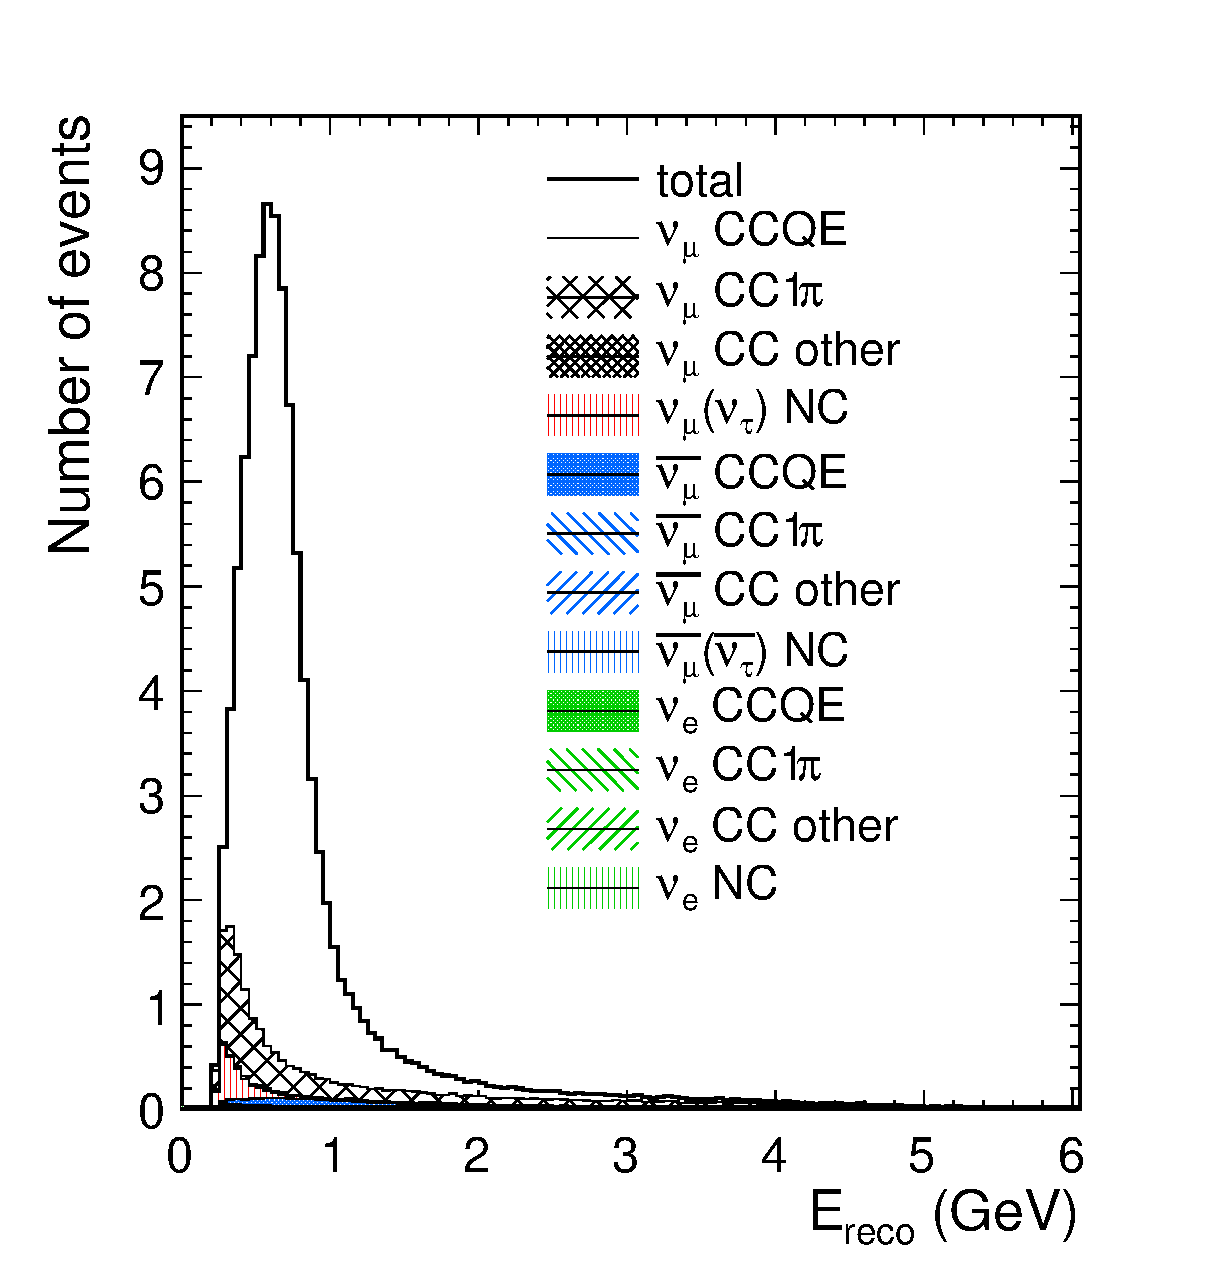
\includegraphics[width=19pc,height=19pc]{./images/predicted_spectrum/nominal/genie_contrib_noosc.eps}
\caption{
  Predicted non-oscillated reconstructed-energy spectrum of 1 $\mu$-like ring events (after extrapolation)
  and contributions from various true neutrino reaction modes (GENIE)
}
\label{fig:genie_mode_contrib_noosc}
\end{minipage}
\hspace{0.04\linewidth}
\begin{minipage}[t]{0.48\linewidth}
\centering
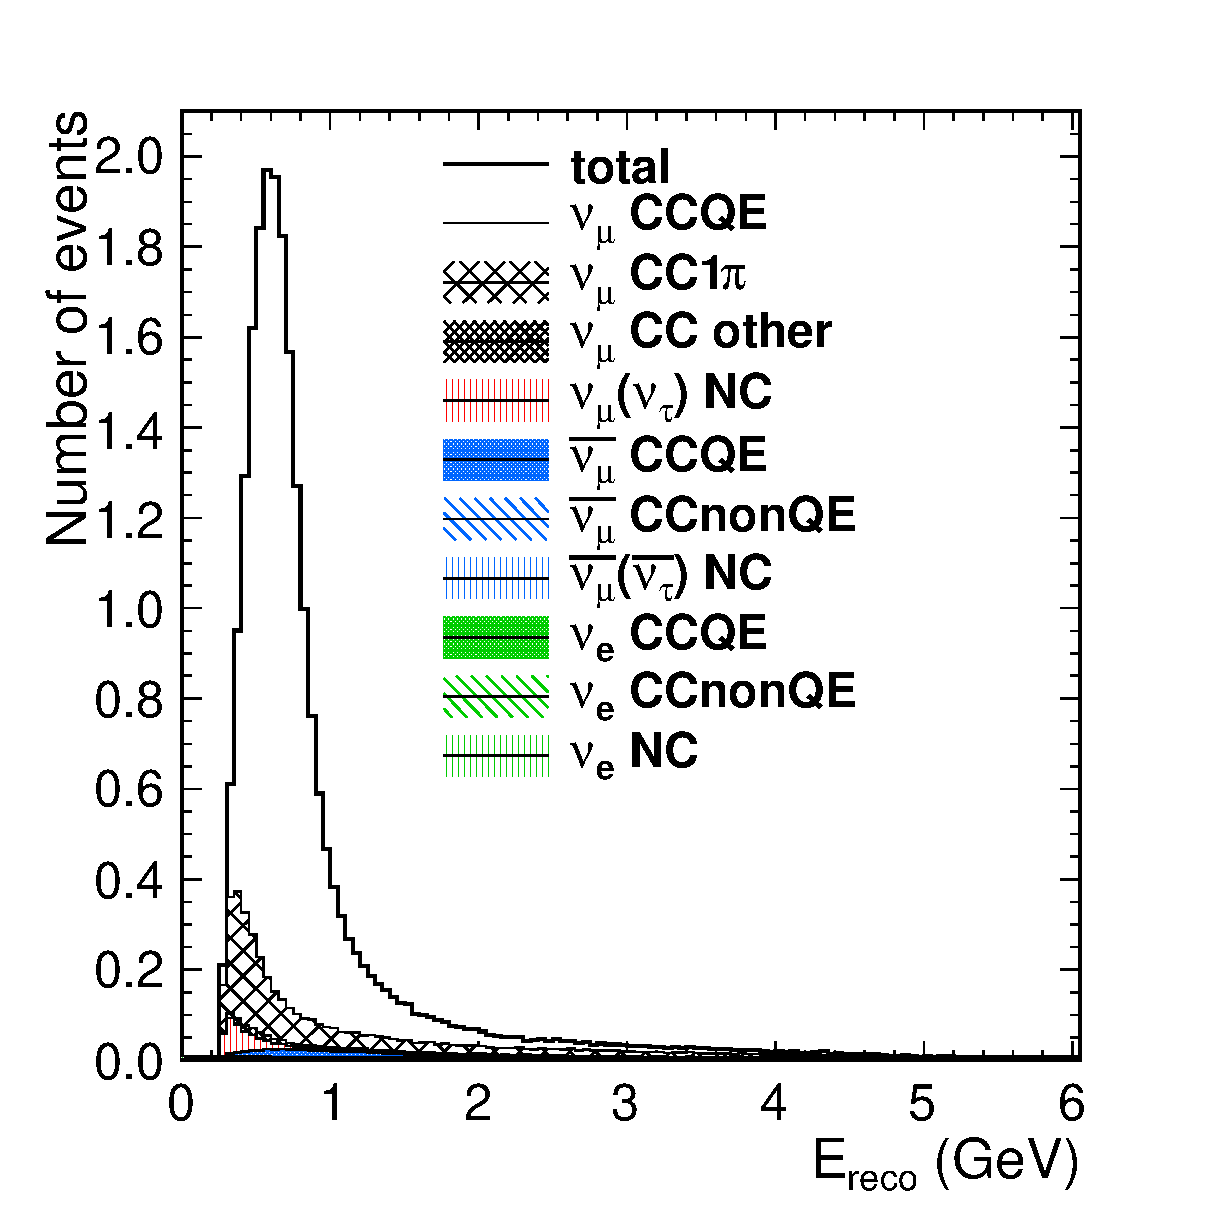
\includegraphics[width=19.5pc,height=19pc]{images/predicted_spectrum/nominal/neut_contrib_noosc.eps}
\caption{
  Predicted non-oscillated reconstructed-energy spectrum of 1 $\mu$-like ring events (after extrapolation)
  and contributions from various true neutrino reaction modes (NEUT)
}
\label{fig:neut_mode_contrib_noosc}
\end{minipage}
\end{figure}


% as above but in log-scale

\begin{figure}[ht]
\begin{minipage}[t]{0.48\linewidth}
\centering
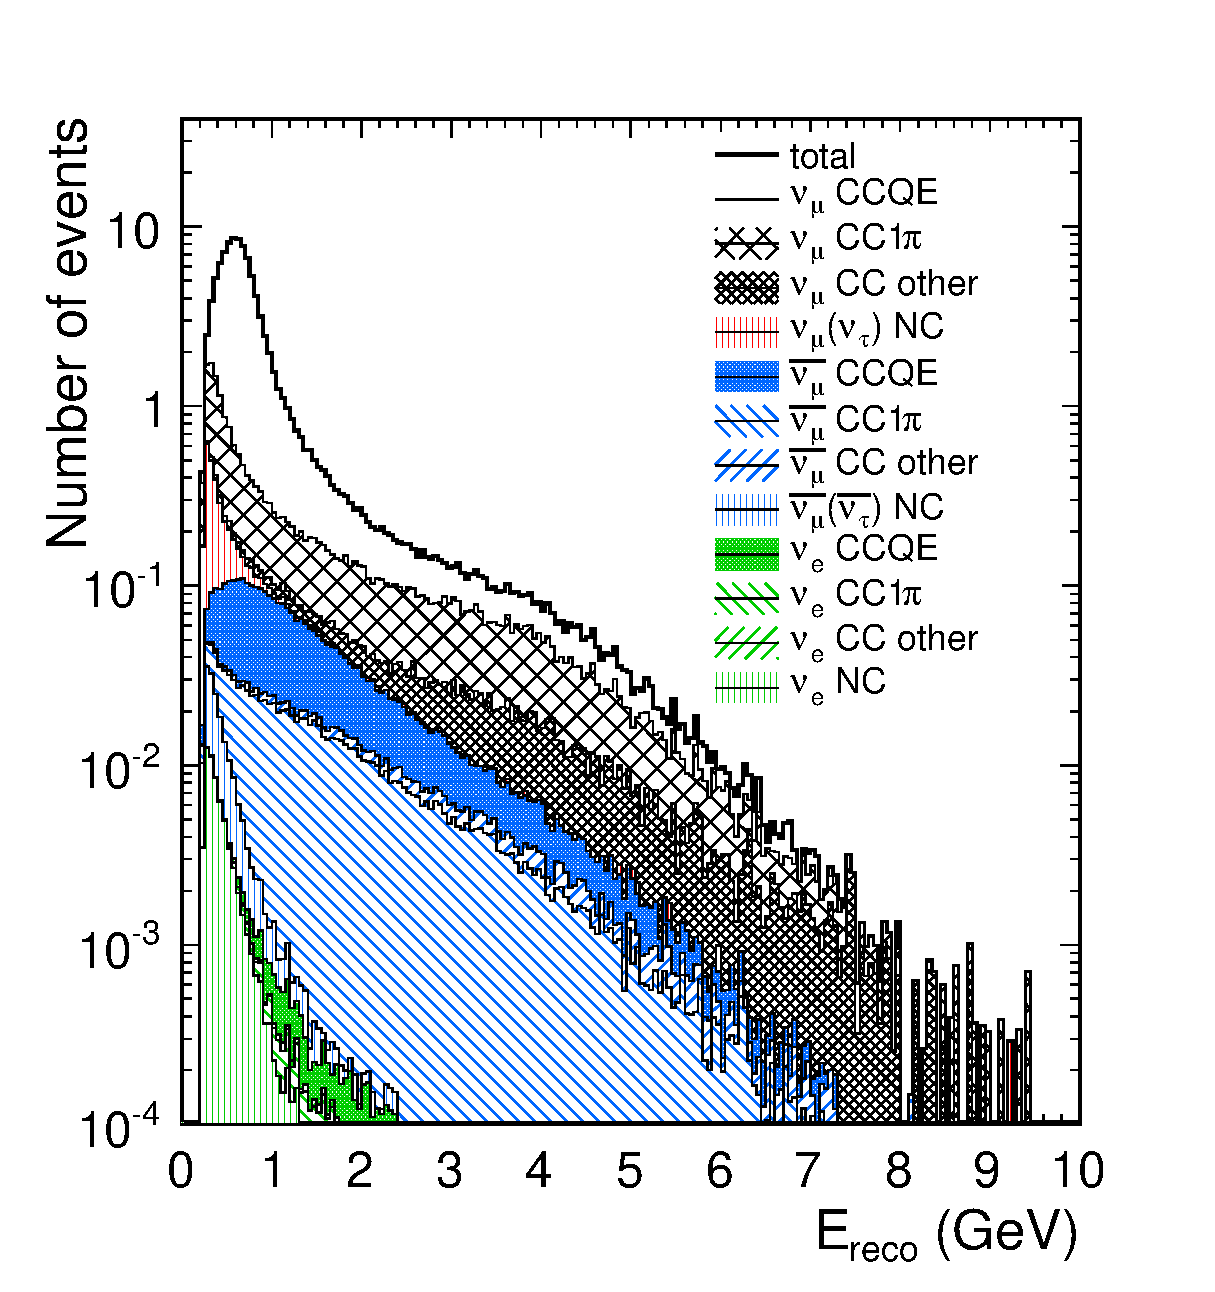
\includegraphics[width=19pc,height=19pc]{./images/predicted_spectrum/nominal/genie_contrib_noosc_logy.eps}
\caption{
  Predicted non-oscillated reconstructed-energy spectrum of 1 $\mu$-like ring events (after extrapolation)
  and contributions from various true neutrino reaction modes (GENIE)
}
\label{fig:genie_mode_contrib_noosc_logy}
\end{minipage}
\hspace{0.04\linewidth}
\begin{minipage}[t]{0.48\linewidth}
\centering
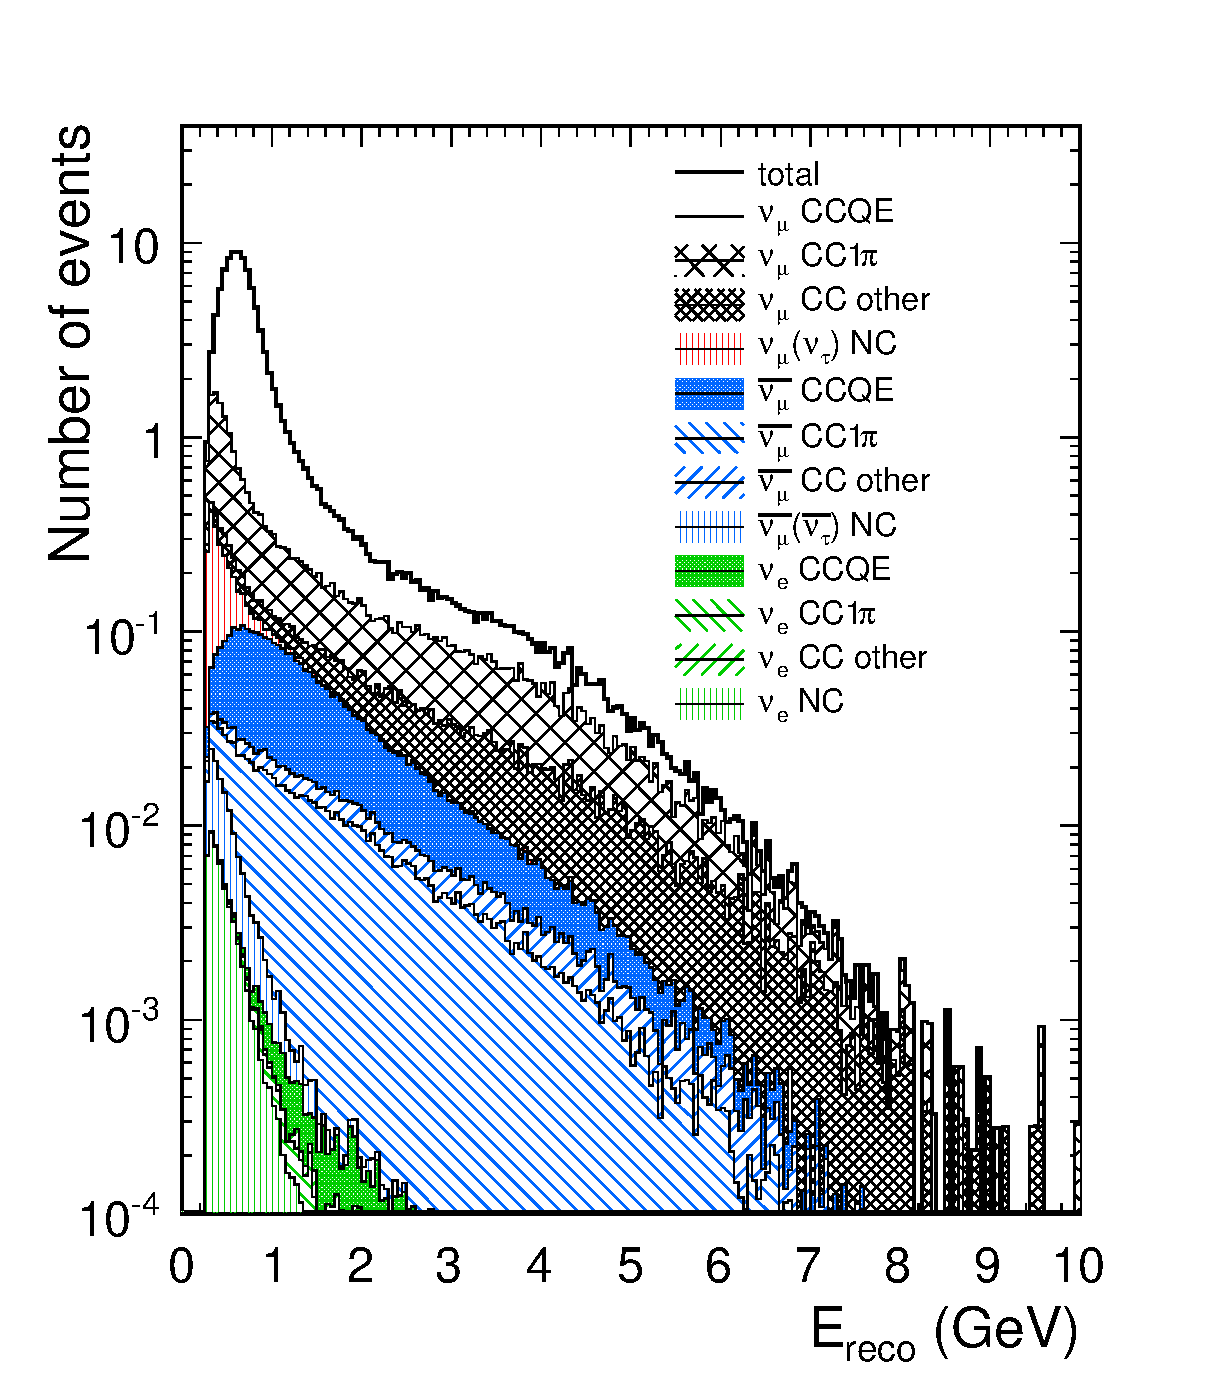
\includegraphics[width=19.5pc,height=19pc]{images/predicted_spectrum/nominal/neut_contrib_noosc_logy.eps}
\caption{
  Predicted non-oscillated reconstructed-energy spectrum of 1 $\mu$-like ring events (after extrapolation)
  and contributions from various true neutrino reaction modes (NEUT)
}
\label{fig:neut_mode_contrib_noosc_logy}
\end{minipage}
\end{figure}


%
% GENIE and NEUT 1-ring Ereco spectrum: MINOS-2011 oscillation params
%

\begin{figure}[ht]
\begin{minipage}[t]{0.48\linewidth}
\centering
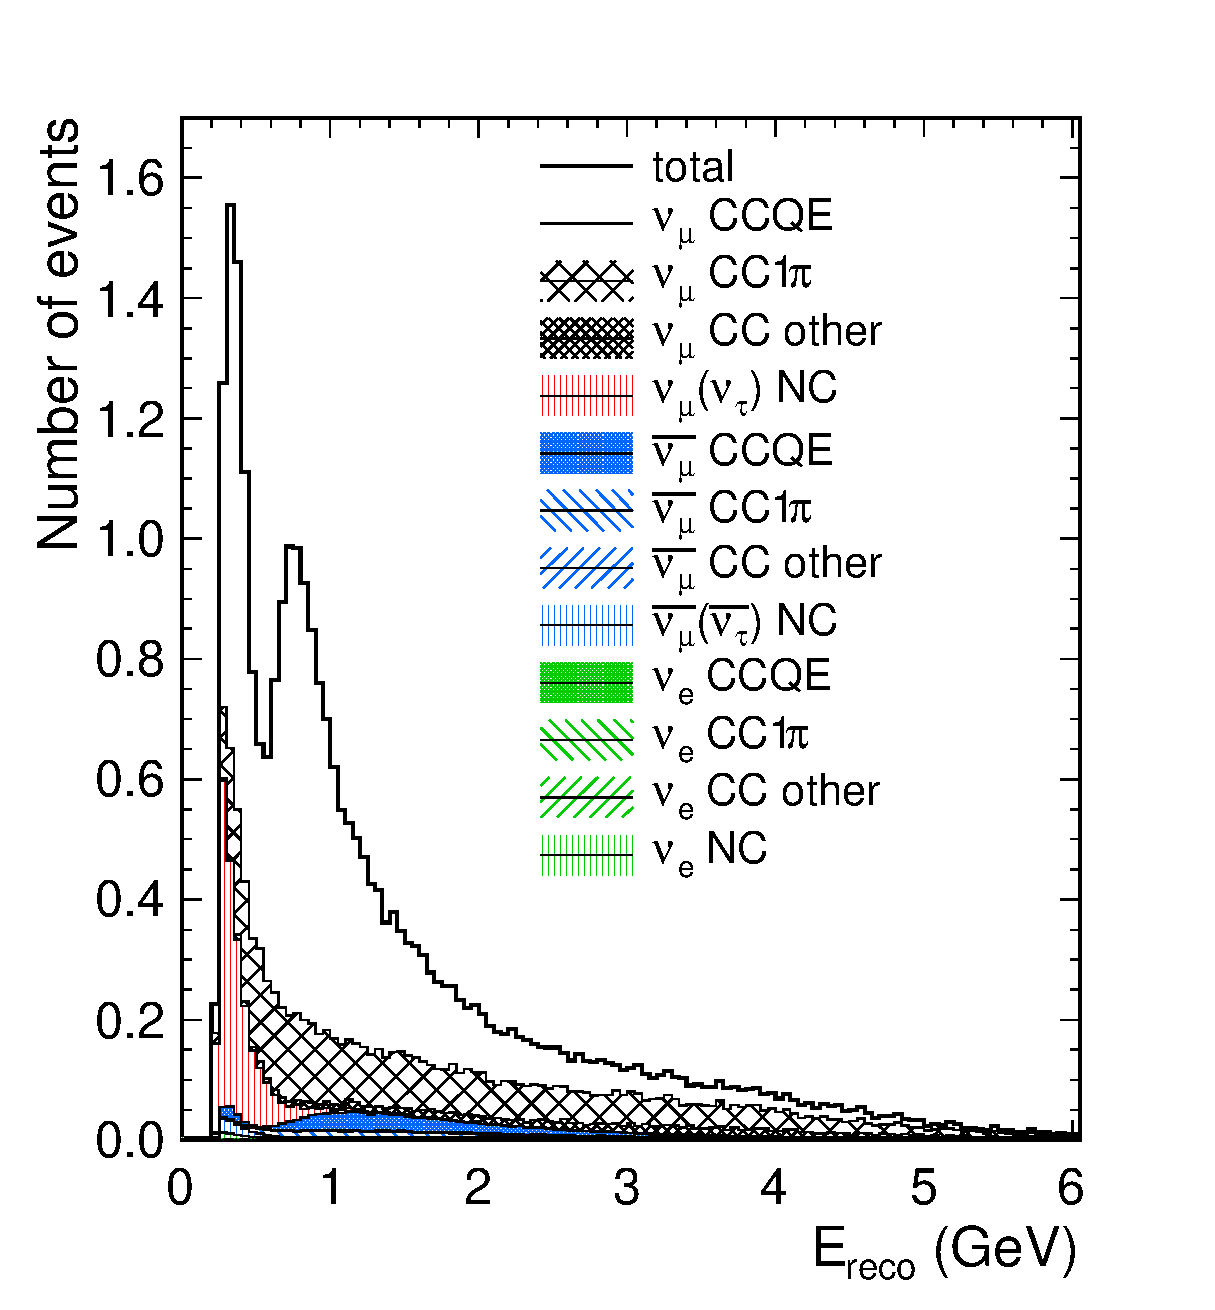
\includegraphics[width=19pc,height=19pc]{./images/predicted_spectrum/nominal/genie_contrib_2p32Em3_1p0.eps}
\caption{
  Predicted oscillated ($sin^{2}2\theta_{23}$ = 1.0 and $|\Delta m^{2}_{23}|$ = 2.32$\times10^{-3}$ $eV^{2}/c^{4}$)
  reconstructed-energy spectrum of 1 $\mu$-like ring events (after extrapolation)
  and contributions from various true neutrino reaction modes (GENIE)
}
\label{fig:genie_mode_contrib_2p32Em3_1p0}
\end{minipage}
\hspace{0.04\linewidth}
\begin{minipage}[t]{0.48\linewidth}
\centering
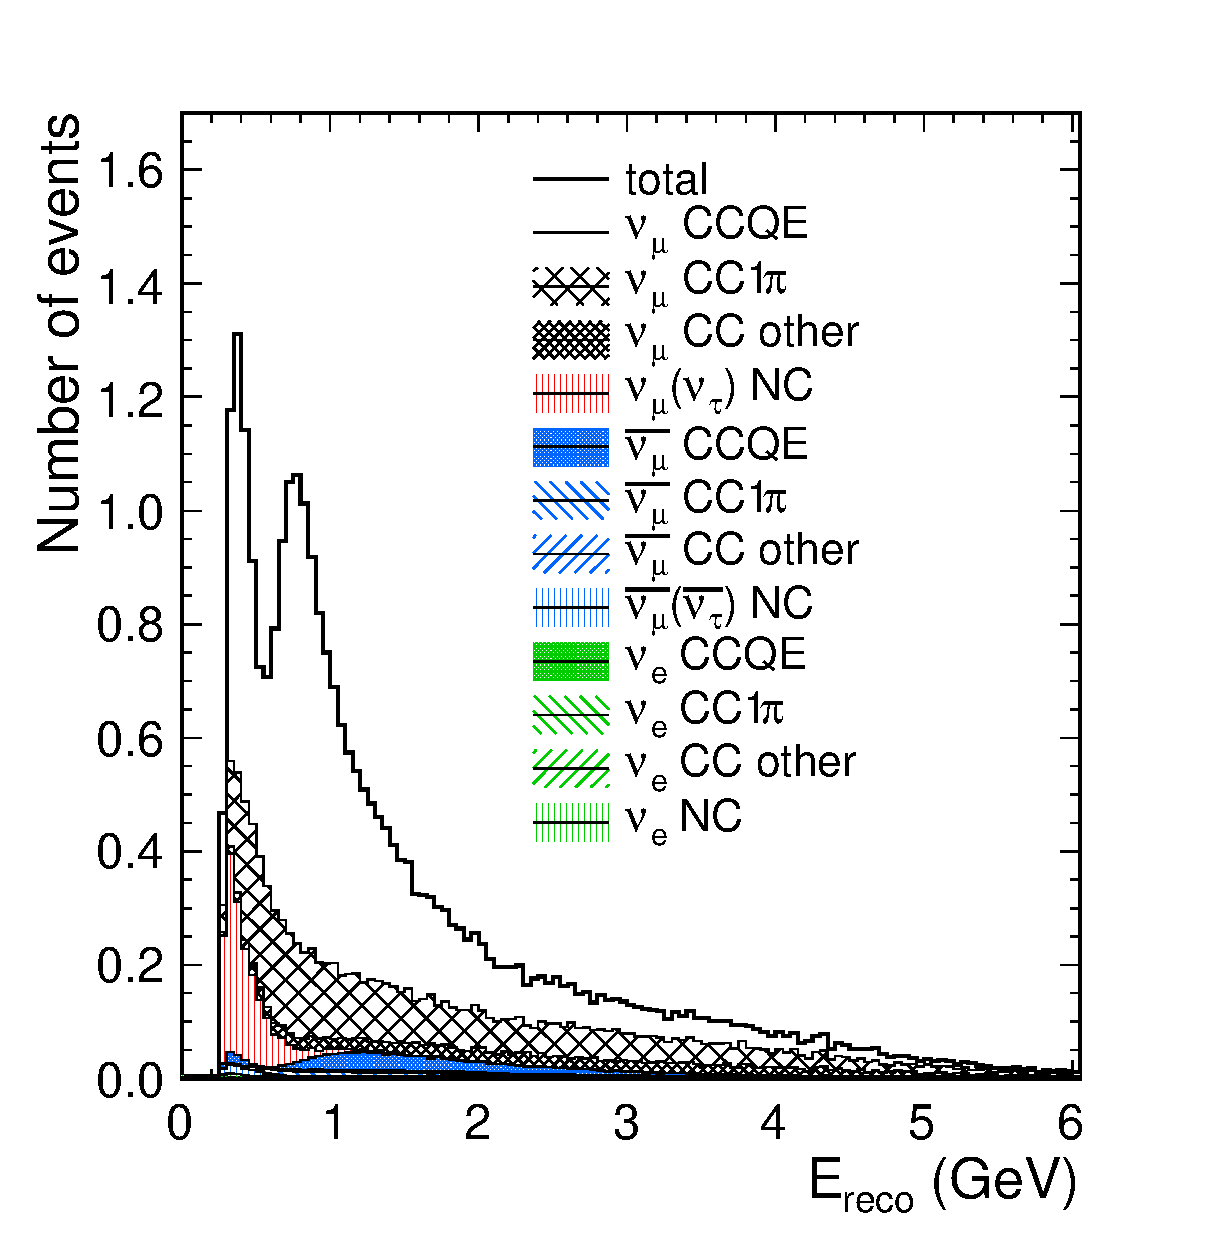
\includegraphics[width=19pc,height=19pc]{images/predicted_spectrum/nominal/neut_contrib_2p32Em3_1p0.eps}
\caption{
  Predicted oscillated ($sin^{2}2\theta_{23}$ = 1.0 and $|\Delta m^{2}_{23}|$ = 2.32$\times10^{-3}$ $eV^{2}/c^{4}$)
  reconstructed-energy spectrum of 1 $\mu$-like ring events (after extrapolation)
  and contributions from various true neutrino reaction modes (NEUT)
}
\label{fig:neut_mode_contrib_2p32Em3_1p0}
\end{minipage}
\end{figure}


% as above but in log-scale

\begin{figure}[ht]
\begin{minipage}[t]{0.48\linewidth}
\centering
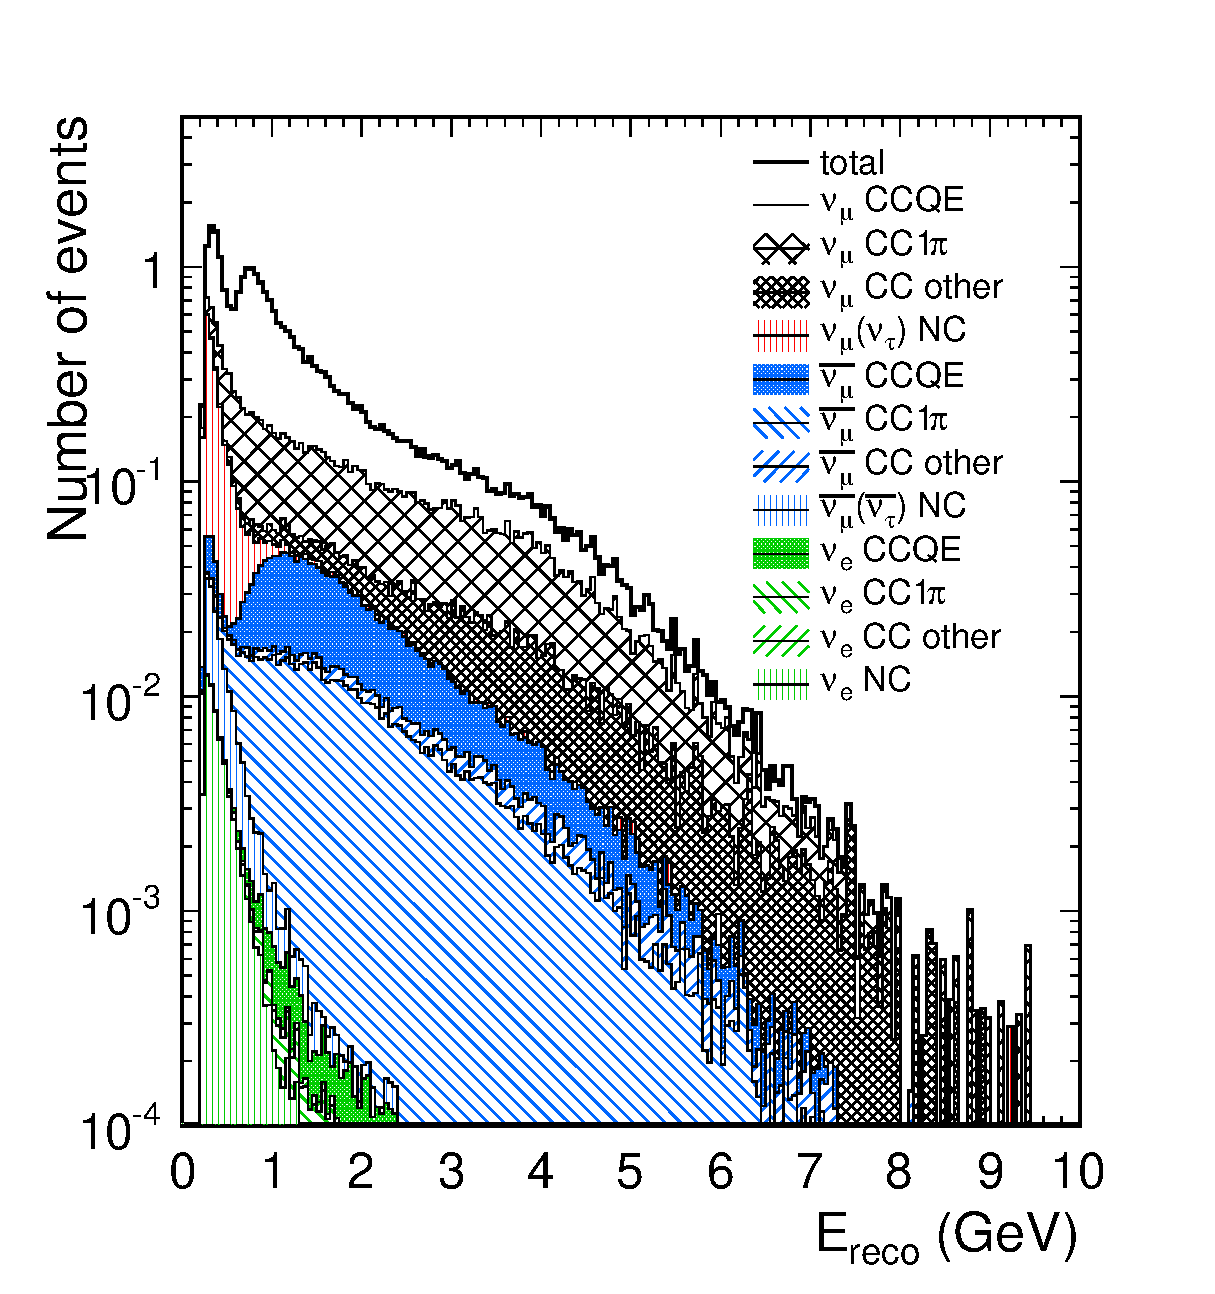
\includegraphics[width=19pc,height=19pc]{./images/predicted_spectrum/nominal/genie_contrib_2p32Em3_1p0_logy.eps}
\caption{
  Predicted oscillated ($sin^{2}2\theta_{23}$ = 1.0 and $|\Delta m^{2}_{23}|$ = 2.32$\times10^{-3}$ $eV^{2}/c^{4}$)
  reconstructed-energy spectrum of 1 $\mu$-like ring events (after extrapolation)
  and contributions from various true neutrino reaction modes (GENIE)
}
\label{fig:genie_mode_contrib_2p32Em3_1p0_logy}
\end{minipage}
\hspace{0.04\linewidth}
\begin{minipage}[t]{0.48\linewidth}
\centering
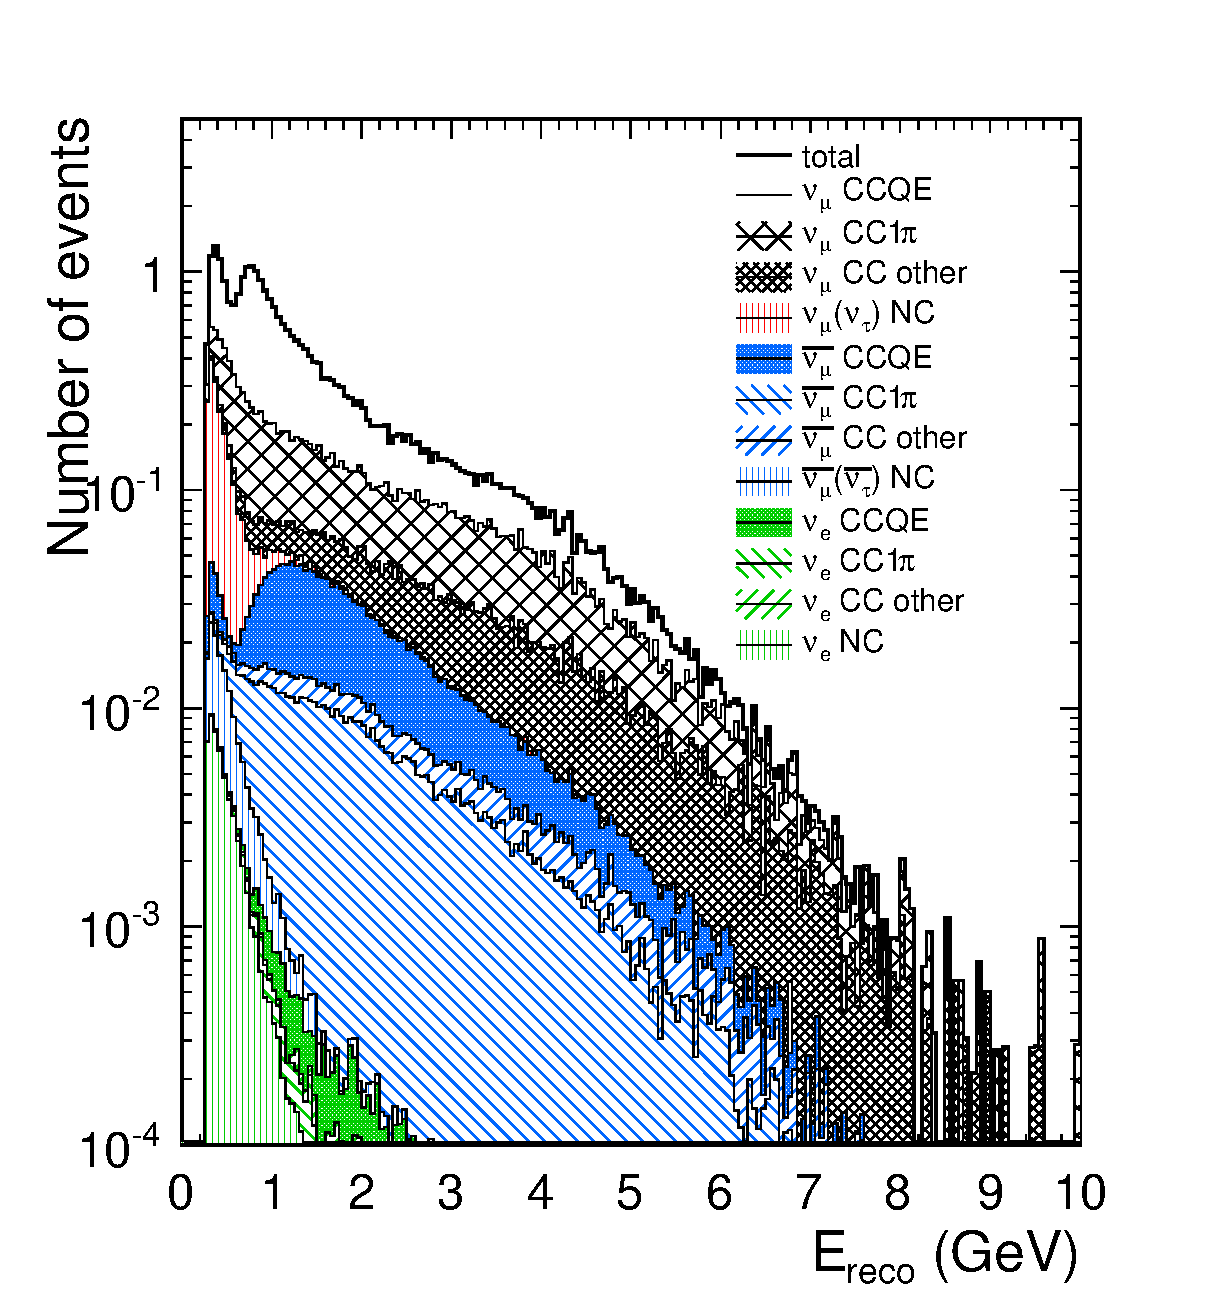
\includegraphics[width=19pc,height=19pc]{images/predicted_spectrum/nominal/neut_contrib_2p32Em3_1p0_logy.eps}
\caption{
  Predicted oscillated ($sin^{2}2\theta_{23}$ = 1.0 and $|\Delta m^{2}_{23}|$ = 2.32$\times10^{-3}$ $eV^{2}/c^{4}$)
  reconstructed-energy spectrum of 1 $\mu$-like ring events (after extrapolation)
  and contributions from various true neutrino reaction modes (NEUT)
}
\label{fig:neut_mode_contrib_2p32Em3_1p0_logy}
\end{minipage}
\end{figure}

%
% Nsk vs oscillation parameters
%

\begin{figure}[ht]
\begin{minipage}[t]{0.47\linewidth}
\centering
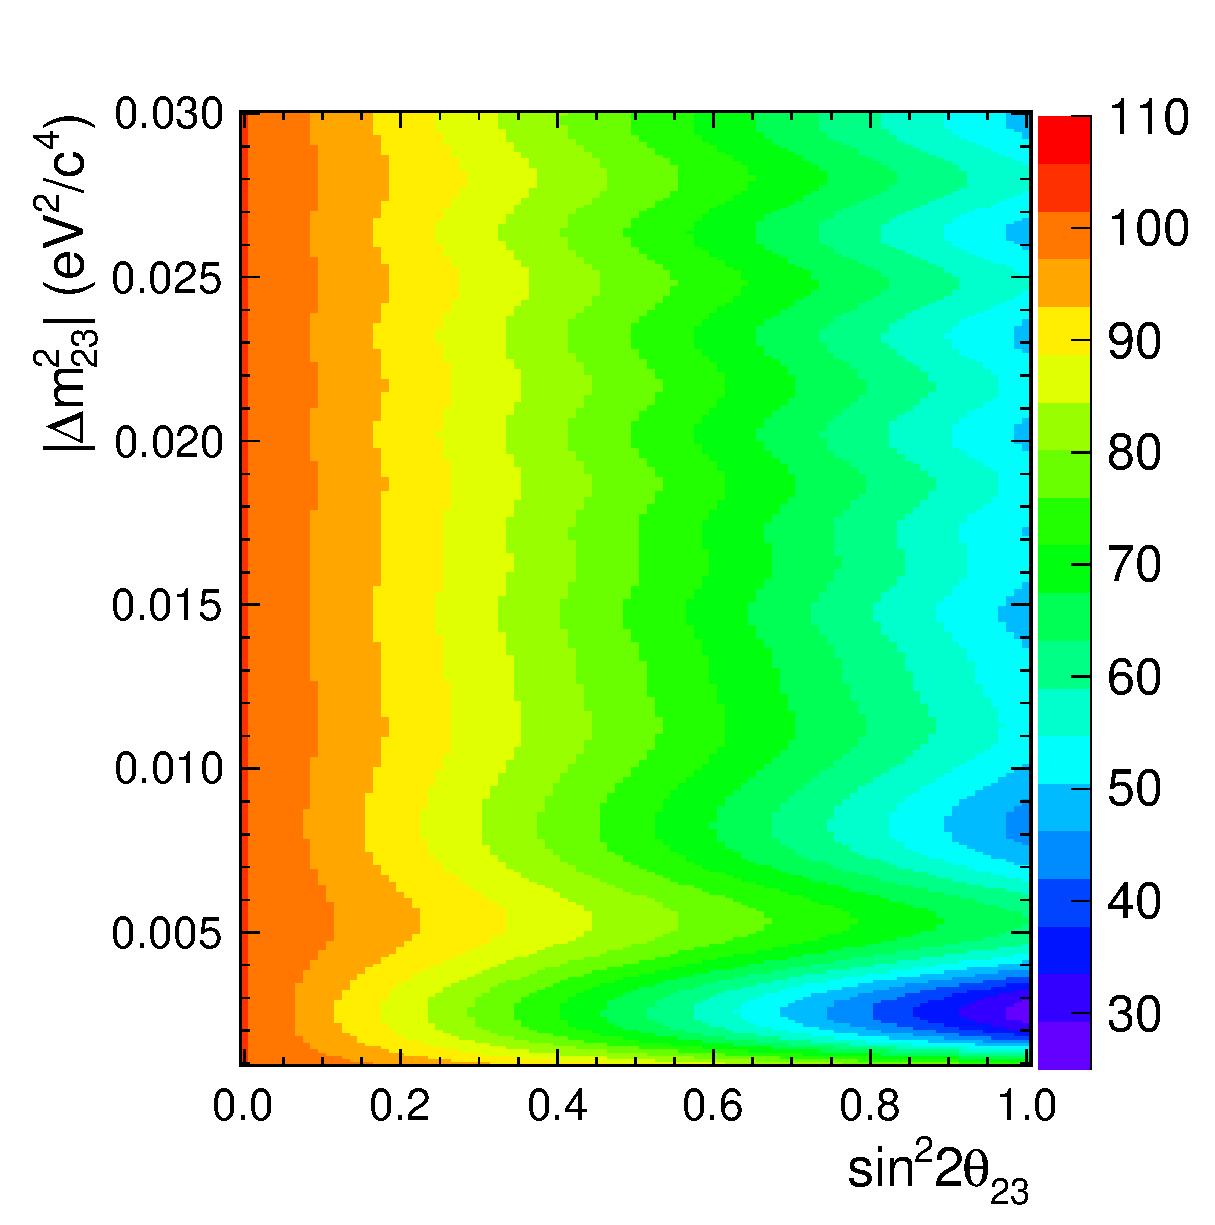
\includegraphics[width=18pc,height=19pc]{./images/predicted_spectrum/nominal/genie_nsk_osc.eps}
\caption{
  Expected number of 1 $\mu$-like ring events (after extrapolation) in the 0-10 GeV reconstructed
  energy range (GENIE)
}
\label{fig:genie_nsk_osc_param_grid}
\end{minipage}
\hspace{0.06\linewidth}
\begin{minipage}[t]{0.47\linewidth}
\centering
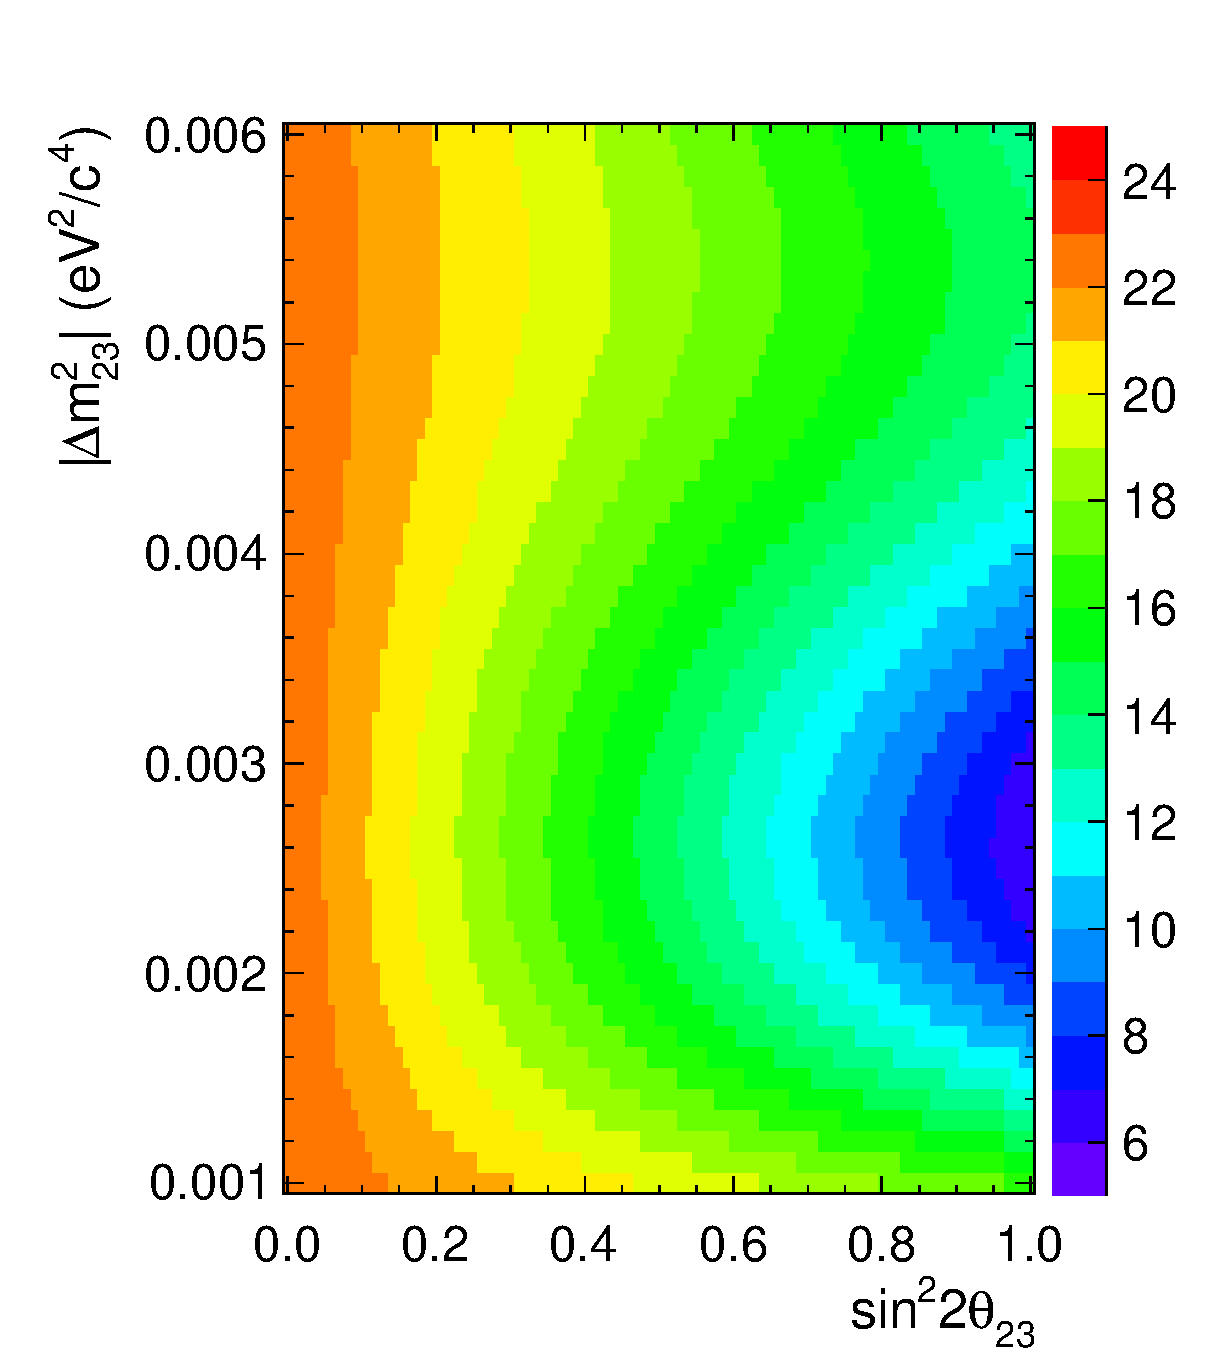
\includegraphics[width=18pc,height=19pc]{images/predicted_spectrum/nominal/neut_nsk_osc.eps}
\caption{
  Expected number of 1 $\mu$-like ring events (after extrapolation) in the 0-10 GeV reconstructed
  energy range (NEUT)
}
\label{fig:neut_nsk_osc_param_grid}
\end{minipage}
\end{figure}


%
% Nsk vs oscillation parameters
%

\begin{figure}[ht]
\begin{minipage}[t]{0.47\linewidth}
\centering
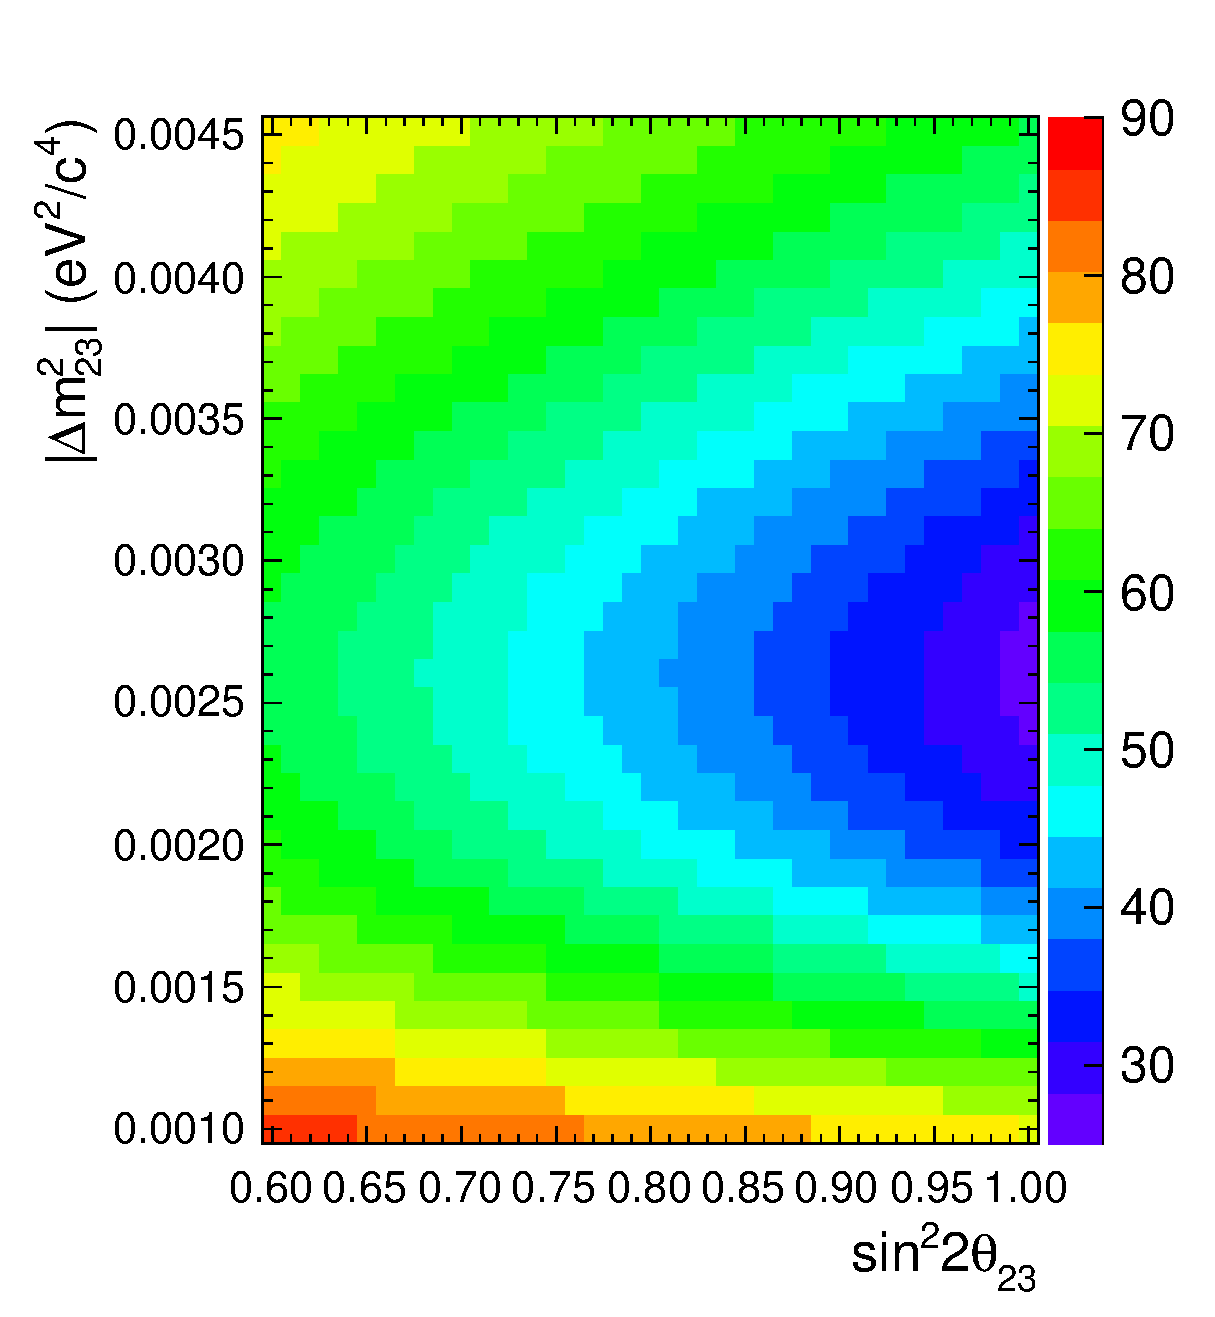
\includegraphics[width=18pc,height=19pc]{./images/predicted_spectrum/nominal/genie_nsk_osc_zoom.eps}
\caption{
  Expected number of 1 $\mu$-like ring events (after extrapolation) in the 0-10 GeV reconstructed
  energy range, zoomed around the MINOS 2011 best-fit values (GENIE)
}
\label{fig:genie_nsk_osc_param_grid_zoom}
\end{minipage}
\hspace{0.06\linewidth}
\begin{minipage}[t]{0.47\linewidth}
\centering
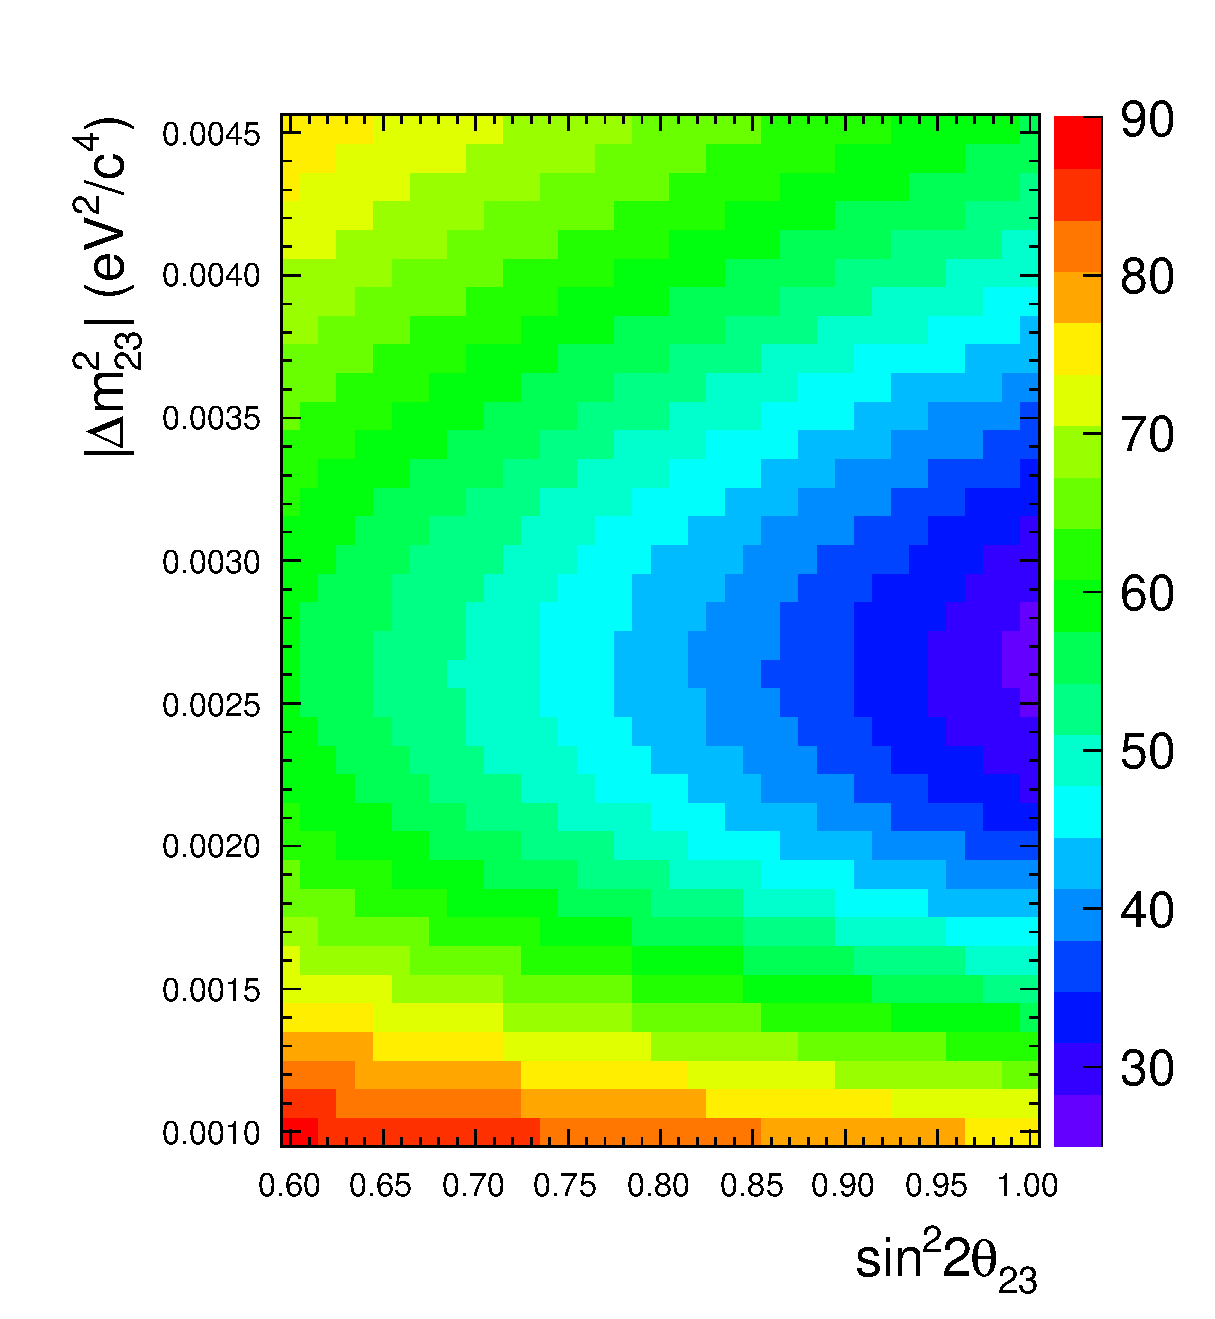
\includegraphics[width=18pc,height=19pc]{images/predicted_spectrum/nominal/neut_nsk_osc_zoom.eps}
\caption{
  Expected number of 1 $\mu$-like ring events (after extrapolation) in the 0-10 GeV reconstructed
  energy range, zoomed around the MINOS 2011 best-fit values (NEUT)
}
\label{fig:neut_nsk_osc_param_grid_zoom}
\end{minipage}
\end{figure}

\begin{table*}[htb]
\center
\renewcommand{\arraystretch}{1.75} % enlarge line spacing
\begin{tabular}{|c|c|c|}
\hline
       & GENIE & NEUT \\
Error source  &
  $\delta{N^{exp}_{SK}}/N^{exp}_{SK}$  &
  $\delta{N^{exp}_{SK}}/N^{exp}_{SK}$  \\
\hline
SuperK CCQE efficiency (ring-counting)  &   $\pm$2.99\%       &   $\pm$3.06\%       \\
SuperK CCQE efficiency (other)          &   $\pm$1.41\%       &   $\pm$1.39\%       \\
SuperK CCnonQE efficiency               &   $\pm$2.99\%       &   $\pm$3.32\%       \\
SuperK NC efficiency                    &   $\pm$2.51\%       &   $\pm$1.96\%       \\
SuperK $\nu_{e}$ CC efficiency          &   $\pm$0.01\%       &   $\pm$0.01\%       \\
ND280 efficiency                        &   +5.49\% -5.30\%   &   +5.49\% -5.30\%   \\
ND280 normalization                     &   $\pm$2.63\%       &   $\pm$2.62\%       \\
Flux normalization                      &   $\pm$7.29\%       &   $\pm$7.33\%       \\
CCQE cross section                      &   $\pm$4.28\%       &   $\pm$4.05\%       \\
CC1pi/CCQE cross section ratio          &   +2.66\% -2.35\%   &   +2.18\% -1.93\%   \\
CCother/CCQE cross section ratio        &   +5.80\% -5.16\%   &   +5.27\% -4.71\%   \\ 
NC/CCQE cross section ratio             &   +0.68\% -0.66\%   &   +0.81\% -0.78\%   \\
FSI                                     &   $\pm$3.23\%       &   $\pm$3.22\%       \\
\hline
Total                                   &   +13.65\% -13.26\% &   +13.30\% -12.97\% \\
\hline
\end{tabular}\\[2pt]
\caption{
  Effect of 1$\sigma$ systematic parameter variation on the non-oscillated number of 1 $\mu$-like ring events
  predicted by GENIE and NEUT (after extrapolation)
}
\label{table:dnsk_noosc}
\end{table*}



\begin{table*}[htb]
\center
\renewcommand{\arraystretch}{1.75} % enlarge line spacing
\begin{tabular}{|c|c|c|}
\hline
       & GENIE & NEUT \\
Error source  &
  $\delta{N^{exp}_{SK}}/N^{exp}_{SK}$  &
  $\delta{N^{exp}_{SK}}/N^{exp}_{SK}$  \\
\hline
SuperK CCQE efficiency (ring-counting)  &   $\pm$3.04\%       &   $\pm$3.23\%       \\
SuperK CCQE efficiency (other)          &   $\pm$1.05\%       &   $\pm$1.04\%       \\
SuperK CCnonQE efficiency               &   $\pm$6.00\%       &   $\pm$6.51\%       \\
SuperK NC efficiency                    &   $\pm$8.97\%       &   $\pm$6.96\%       \\
SuperK $\nu_{e}$ CC efficiency          &   $\pm$0.04\%       &   $\pm$0.05\%       \\
ND280 efficiency                        &   +5.49\% -5.30\%   &   +5.59\% -5.30\%   \\
ND280 normalization                     &   $\pm$2.63\%       &   $\pm$2.62\%       \\
Flux normalization                      &   $\pm$4.78\%       &   $\pm$4.73\%       \\
CCQE cross section                      &   $\pm$2.78\%       &   $\pm$2.36\%       \\
CC1pi/CCQE cross section ratio          &   +0.22\% -0.25\%   &   +0.52\% -0.59\%   \\
CCother/CCQE cross section ratio        &   +5.04\% -4.48\%   &   +4.10\% -3.67\%   \\ 
NC/CCQE cross section ratio             &   +1.40\% -1.44\%   &   +0.82\% -0.84\%   \\
FSI                                     &   $\pm$5.68\%       &   $\pm$5.80\%       \\
\hline
Total                                   &   +15.94\% -15.72\% &   +14.79\% -14.61\% \\
\hline
\end{tabular}\\[2pt]
\caption{
  Effect of 1$\sigma$ systematic parameter variation on the number of 1 $\mu$-like ring events
  predicted by GENIE and NEUT (after extarpolation)
  assuming oscillations with typical (MINOS 2011) parameters
  ($sin^{2}2\theta_{23}$ = 1.0 and $|\Delta m^{2}_{23}|$ = 2.32$\times10^{-3}$ $eV^{2}/c^{4}$).
}
\label{table:dnsk_minos11}
\end{table*}


%
% GENIE and NEUT 1-ring Ereco spectrum error envelope
%

\begin{figure}[ht]
\begin{minipage}[t]{0.48\linewidth}
\centering
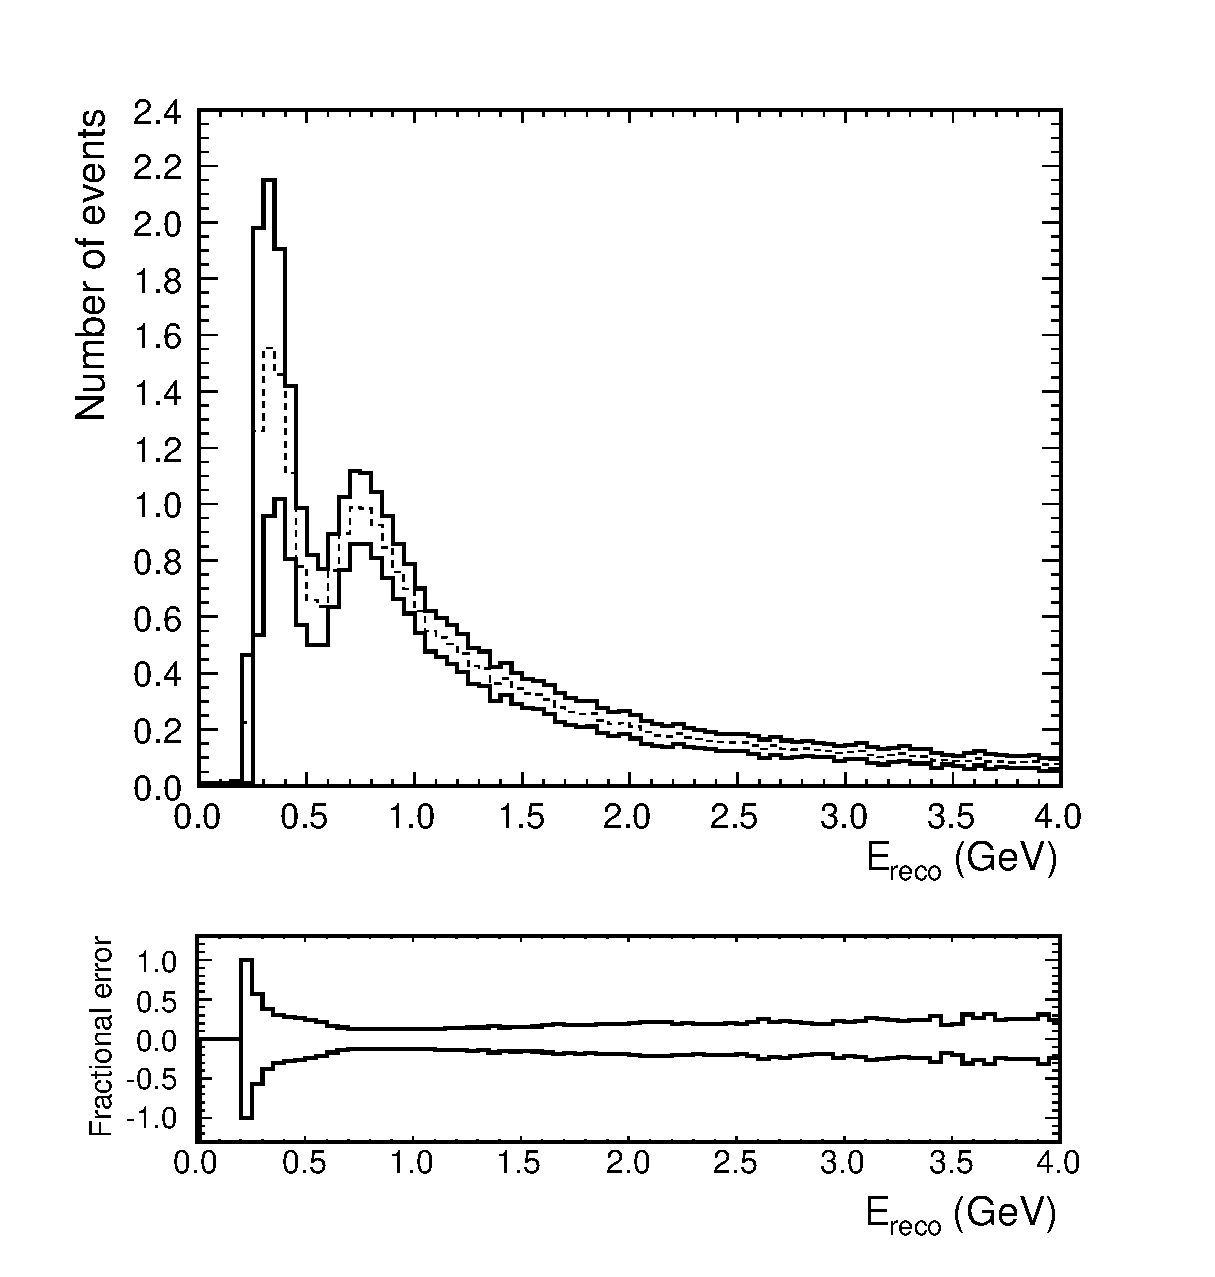
\includegraphics[width=18pc,height=20pc]{./images/predicted_spectrum/systematic_variations/genie-sk-err-envelope-minos11.eps}
\caption{
  Error envelope of 1 $\mu$-like ring event reconstructed-energy spectrum (after extrapolation)
  for oscillations with $sin^{2}2\theta_{23}$ = 1.0 and $|\Delta m^{2}_{23}|$ = 2.32$\times10^{-3}$ $eV^{2}/c^{4}$.
  Calculated from toy MC experiments as the $\pm1\sigma$ spread of bin contents (GENIE).
}
\label{fig:genie-sk-err-envelope-minos11}
\end{minipage}
\hspace{0.04\linewidth}
\begin{minipage}[t]{0.48\linewidth}
\centering
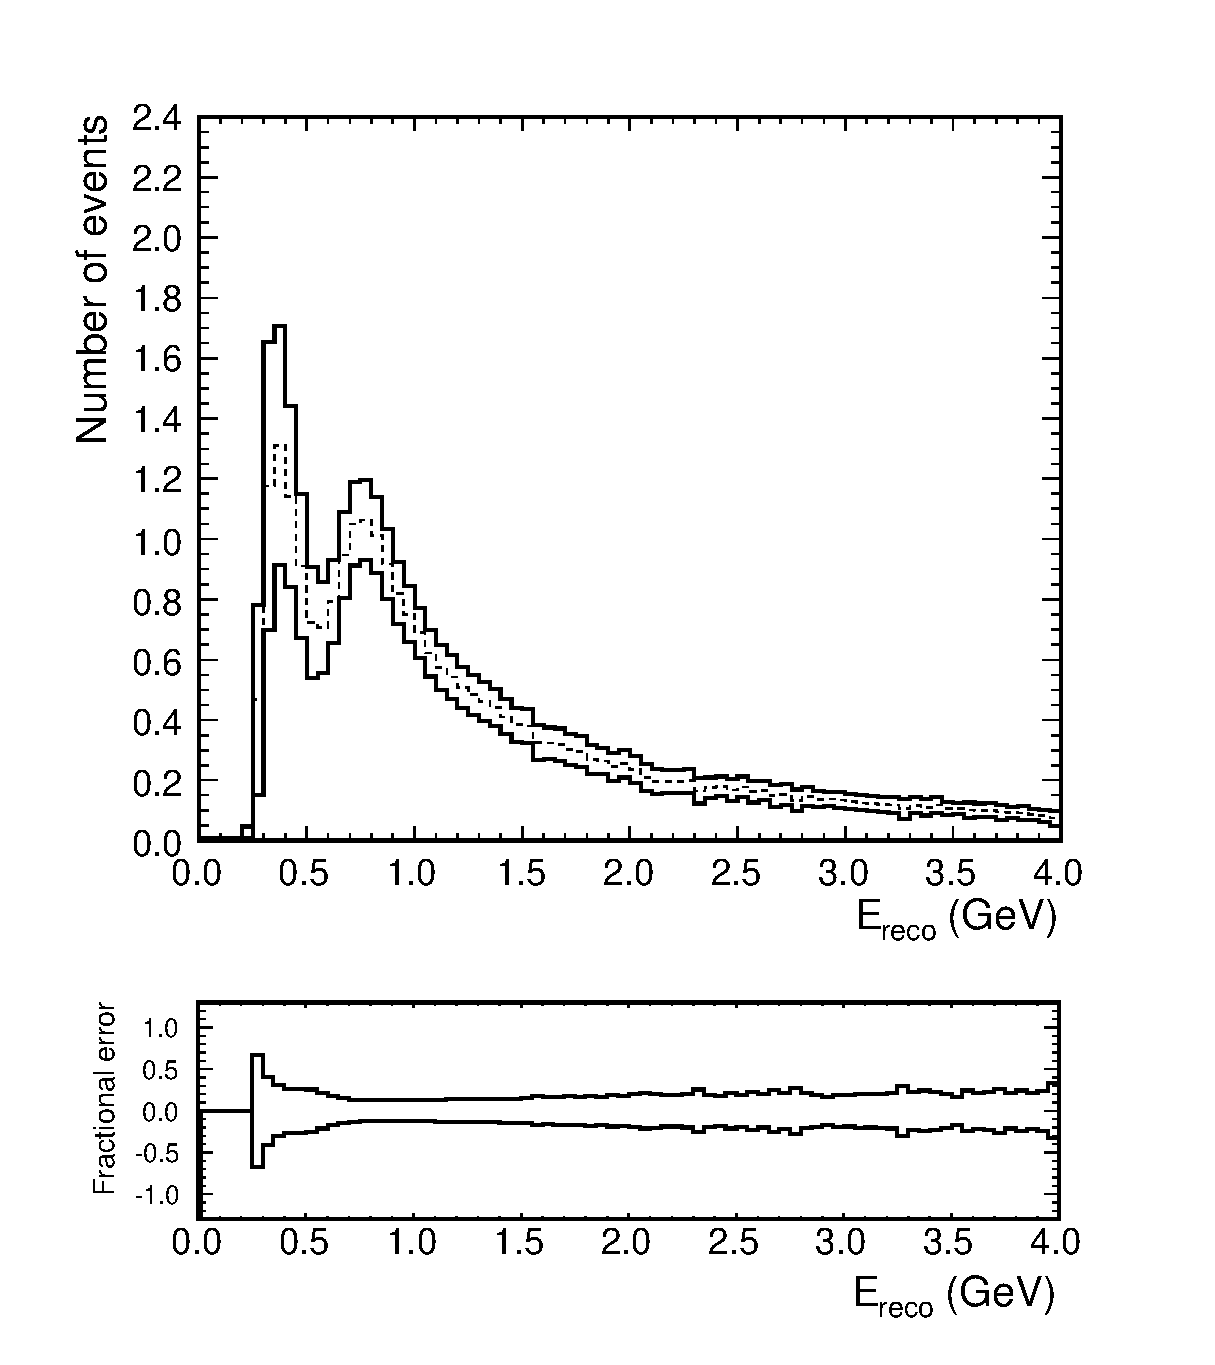
\includegraphics[width=18pc,height=20pc]{images/predicted_spectrum/systematic_variations/neut-sk-err-envelope-minos11.eps}
\caption{
  Error envelope of 1 $\mu$-like ring event reconstructed-energy spectrum (after extrapolation)
  for oscillations with $sin^{2}2\theta_{23}$ = 1.0 and $|\Delta m^{2}_{23}|$ = 2.32$\times10^{-3}$ $eV^{2}/c^{4}$.
  Calculated from toy MC experiments as the $\pm1\sigma$ spread of bin contents (NEUT).
}
\label{fig:neut-sk-err-envelope-minos11}
\end{minipage}
\end{figure}

\clearpage

\section {2-flavour $\nu_{\mu}$-disappearance fits to the Run1, Run2 and Run1+2 datasets}
\label{sec:fits}

Using the method outlined in the previous sections and in Ref.\ \cite{OurRun1DisappAnalysis},
a 2-flavour $\nu_{\mu}$-disappearance fit was performed on the $1.431\times10^{20}$ POT Run1+2 dataset.
For GENIE, this analysis found
$|\Delta m^{2}_{23}|$ = 2.60$\times$10$^{-3}$ $eV^{2}/c^{4}$ and
$sin^{2}2\theta_{23}$ = 0.97 
to be the best-fit values ($\chi^{2}/ndf$=0.310).
For NEUT, the corresponding best-fit values were
$|\Delta m^{2}_{23}|$ = 2.65$\times$10$^{-3}$ $eV^{2}/c^{4}$ and
$sin^{2}2\theta_{23}$ = 0.98 ($\chi^{2}/ndf$=0.311).
The reconstructed neutrino energy distribution of the 31 single $\mu$-like ring events in the Run1+2 dataset, 
along with the best-fit predictions from GENIE and NEUT, are shown in  
Figs.\ \ref{fig:run1p2_spectrum_and_data_genie} and \ref{fig:run1p2_spectrum_and_data_neut}.
These distributions are shown in the 50 MeV reconstructed neutrino energy bins that were used in the fitting procedure.
It is illuminating to see the same distributions with a smaller number of bins of
 variable size in reconstructed neutrino energy; these are shown in 
Figs.\ \ref{fig:run1p2_spectrum_and_data_genie_rebin} and \ref{fig:run1p2_spectrum_and_data_neut_rebin}, 
though this binning scheme was not used in the analysis.
In Figs.\ \ref{fig:run1p2_spectrum_and_data_genie_rebin_modes} and \ref{fig:run1p2_spectrum_and_data_neut_rebin_modes},
the $\nu_{\mu}$-CCQE component of the best-fit oscillation hypothesis is added to the distributions shown in the previous figures.

The $\Delta\chi^{2}$ distributions
for the fit to the Run1+2 dataset are shown as a function of $sin^{2}2\theta_{23}$ and $|\Delta m^{2}_{23}|$ in
Fig.\ \ref{fig:run1p2_genie_deltachisqsurf_wide} for GENIE and
Fig.\ \ref{fig:run1p2_neut_deltachisqsurf_wide} for NEUT.
Meanwhile zoomed views around the Run1+2 best-fit values of these $\Delta\chi^{2}$ distributions are shown in
Fig.\ \ref{fig:run1p2_genie_deltachisqsurf_zoom} for GENIE and
Fig.\ \ref{fig:run1p2_neut_deltachisqsurf_zoom} for NEUT.
The marginalised $\Delta\chi^{2}$ distributions for the Run1+2 fit are shown in
Fig.\ \ref{fig:run1p2_genie_marginal_deltachisq_wide} for GENIE and
Fig.\ \ref{fig:run1p2_neut_marginal_deltachisq_wide} for NEUT.
The 1-dimensional marginalised $\Delta\chi^{2}$ distributions are obtained by minimizing $\Delta\chi^{2}$ with respect to
$sin^{2}2\theta_{23}$ for each $|\Delta m^{2}_{23}|$ bin (and vice versa).

Comparisons of the Run1+2 best-fit values with distributions obtained by
2-flavour $\nu_{\mu}$-disappearance 
fits on 1.431$\times$10$^{20}$ POT toy MC experiments 
generated with $sin^{2}2\theta_{23}$ = 1.0 and 
$|\Delta m^{2}_{23}|$ = 2.32$\times10^{-3}$ $eV^{2}/c^{4}$ are shown 
in Figs. \ref{fig:genie-minos11-run1p2-toymc-chisq-distribution} and 
\ref{fig:genie-minos11-run1p2-toymc-bestfitparam-distributions} for GENIE and
in Figs. \ref{fig:neut-minos11-run1p2-toymc-chisq-distribution} and 
\ref{fig:neut-minos11-run1p2-toymc-bestfitparam-distributions} for NEUT.

For comparison, we performed the same 2-flavour $\nu_{\mu}$-disappearance fit separately on the 
$0.323\times10^{20}$-POT Run1 and $1.108\times10^{20}$-POT Run2 datasets.
A summary of the best-fit values for all fits is given in Table \ref{table:bestfit_params_summary}.
The reconstructed neutrino energy spectrum for Run1 (Run2) 1 $\mu$-like ring events 
along with the best-fit and null hypothesis predictions from GENIE are shown in 
Fig.\ \ref{fig:run1_spectrum_and_data_genie_rebin_modes} (Fig.\ \ref{fig:run2_spectrum_and_data_genie_rebin_modes}).
The corresponding Run1 (Run2) distributions for NEUT are shown in
Fig.\ \ref{fig:run1_spectrum_and_data_neut_rebin_modes} (Fig.\ \ref{fig:run2_spectrum_and_data_neut_rebin_modes}).

The marginalised $\Delta\chi^{2}$ distributions for the 2-flavour
$\nu_{\mu}$-disappearance fits to the Run1, Run2 and the combined Run1+2 datasets are shown 
as a function of $sin^{2}2\theta_{23}$ in
Fig.\ \ref{fig:genie_deltachisq_sinsq2theta_3datasets} for GENIE and 
Fig.\ \ref{fig:neut_deltachisq_sinsq2theta_3datasets} for NEUT.
These distributions are also shown as a function of $|\Delta m^{2}_{23}|$ in 
Fig.\ \ref{fig:genie_deltachisq_dmsq_narrow_3datasets} for GENIE and
Fig.\ \ref{fig:neut_deltachisq_dmsq_narrow_3datasets} for NEUT 
(with $|\Delta m^{2}_{23}|$ restricted in the fit to the range
1$\times$10$^{-3}$ $eV^{2}/c^{4}$ - 6$\times$10$^{-3}$ $eV^{2}/c^{4}$).
The effects on these distributions of extending the $|\Delta m^{2}_{23}|$ range to
1$\times$10$^{-3}$ $eV^{2}/c^{4}$ - 30$\times$10$^{-3}$ $eV^{2}/c^{4}$ are
shown in
Fig.\ \ref{fig:genie_deltachisq_dmsq_wide_3datasets} for GENIE and
Fig.\ \ref{fig:neut_deltachisq_dmsq_wide_3datasets} for NEUT.

%
% Summary of best-fit params for the GENIE/NEUT fits to Run1,Run2,Run1+2 fits
%

\begin{table*}[htb]
\center
\renewcommand{\arraystretch}{1.75} % enlarge line spacing
\begin{tabular}{|c||c|c|}
\hline
Dataset                             &  GENIE best-fit values                                         &  NEUT best-fit values   \\
\hline
$0.323\times10^{20}$ POT Run1       &   $|\Delta m^{2}_{23}|$ = 2.77 $\times10^{-3}$ $eV^{2}/c^{4}$  &  $|\Delta m^{2}_{23}|$ = 2.88 $\times10^{-3}$ $eV^{2}/c^{4}$     \\
                                    &   $sin^{2}2\theta_{23}$ = 0.81                                 &  $sin^{2}2\theta_{23}$ = 0.84 \\
                                    &   $\chi^{2}/ndf$ = 0.105                                       &  $\chi^{2}/ndf$ = 0.114 \\
                                    &   (MINOS 2011 params $\chi^{2}/ndf$ = 0.121)                   &  (MINOS 2011 params $\chi^{2}/ndf$ = 0.129) \\
\hline
$1.108\times10^{20}$ POT Run2       &   $|\Delta m^{2}_{23}|$ = 2.59 $\times10^{-3}$ $eV^{2}/c^{4}$  &  $|\Delta m^{2}_{23}|$ = 2.62 $\times10^{-3}$ $eV^{2}/c^{4}$     \\
                                    &   $sin^{2}2\theta_{23}$ = 1.00                                 &  $sin^{2}2\theta_{23}$ = 1.00 \\
                                    &   $\chi^{2}/ndf$ = 0.318                                       &  $\chi^{2}/ndf$ = 0.310 \\
                                    &   (MINOS 2011 params $\chi^{2}/ndf$ = 0.327)                   &  (MINOS 2011 params $\chi^{2}/ndf$ = 0.322) \\
\hline
$1.431\times10^{20}$ POT Run1+2     &   $|\Delta m^{2}_{23}|$ = 2.60 $\times10^{-3}$ $eV^{2}/c^{4}$  &  $|\Delta m^{2}_{23}|$ = 2.65 $\times10^{-3}$ $eV^{2}/c^{4}$     \\
                                    &   $sin^{2}2\theta_{23}$ = 0.97                                 &  $sin^{2}2\theta_{23}$ = 0.98 \\
                                    &   $\chi^{2}/ndf$ = 0.310                                       &  $\chi^{2}/ndf$ = 0.311 \\
                                    &   (MINOS 2011 params $\chi^{2}/ndf$ = 0.319)                   &  (MINOS 2011 params $\chi^{2}/ndf$ = 0.322) \\
\hline
\end{tabular}\\[2pt]
\caption{
  Summary of best-fit parameter values for 2-flavour oscillation fits to the Run1, Run2 and the combined Run1+2 datasets.
  The $\chi^{2}/ndf$ ($ndf$=198) value is also given assuming the MINOS 2011 best-fit parameters
  ($sin^{2}2\theta_{23}$ = 1.0 and $|\Delta m^{2}_{23}|$ = 2.32$\times10^{-3}$ $eV^{2}/c^{4}$).
}
\label{table:bestfit_params_summary}
\end{table*}
  


%
% .....................................................................................................................
%

\clearpage

%
% Run1+2 fit data/best-fit distribution (50 MeV binning)
%

\begin{figure*}[htb]
\center
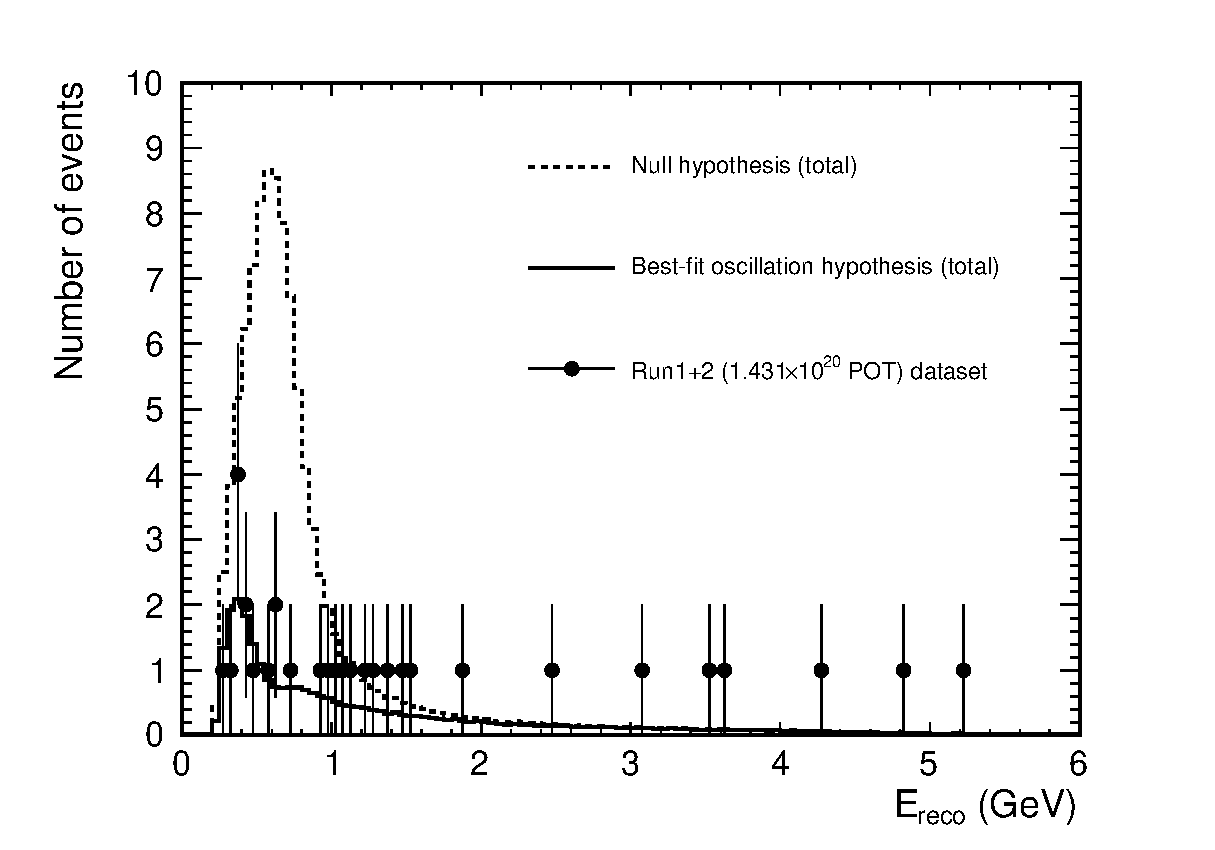
\includegraphics[width=30pc,height=19pc]{./images/fits/run1p2_genie_bestfit_spectrum.eps}
\caption{
  Reconstructed neutrino energy distribution of the 31 single $\mu$-like ring events of the combined
  1.431$\times$10$^{20}$ POT Run1+2 dataset (points) and GENIE best-fit SuperK prediction (solid line).
  The distributions are shown using the 50 MeV reconstructed neutrino energy binning used in the fitting procedure.
  The best-fit oscillation parameters are
  $|\Delta m^{2}_{23}|$ = 2.60$\times$10$^{-3}$ $eV^{2}/c^{4}$ and $sin^{2}2\theta_{23}$ = 0.97.
  The dotted line shows the GENIE prediction without oscillations.
}
\label{fig:run1p2_spectrum_and_data_genie}
\end{figure*}

\begin{figure*}[htb]
\center
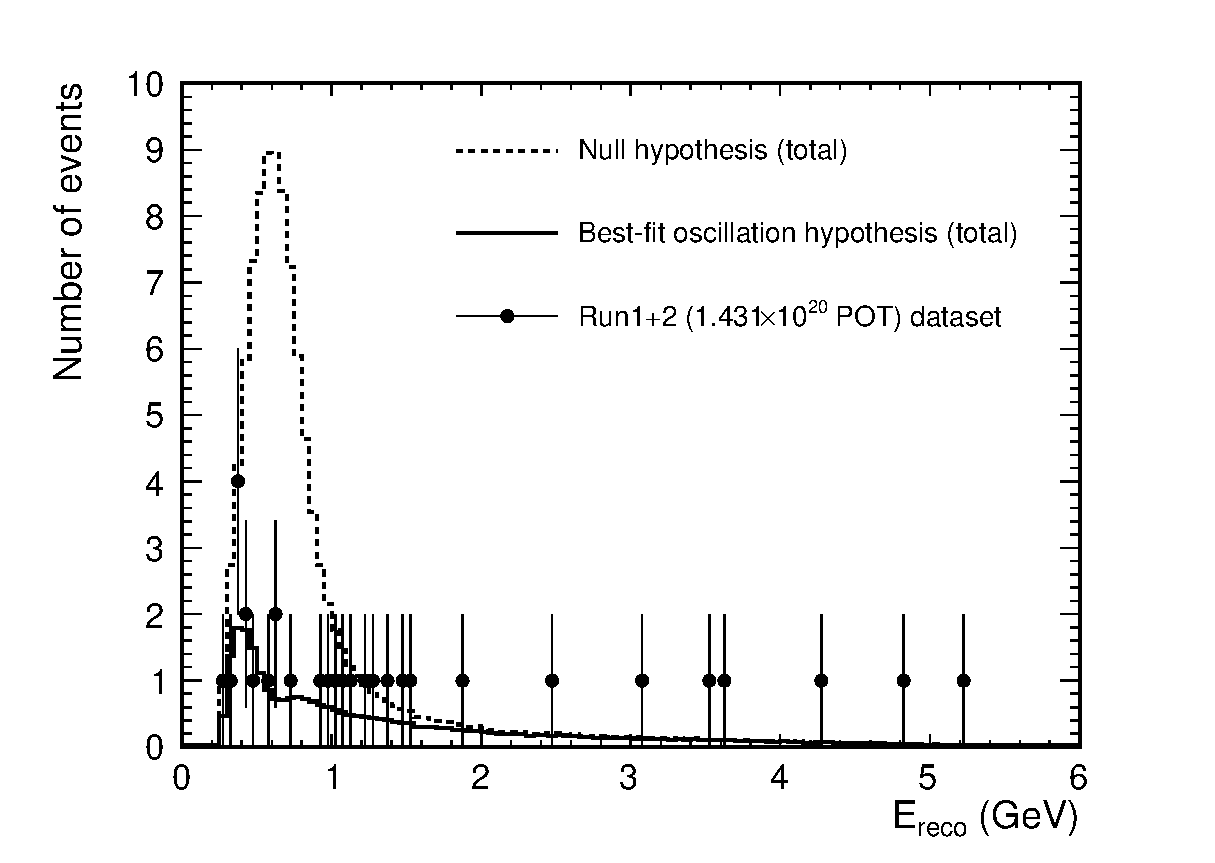
\includegraphics[width=30pc,height=19pc]{./images/fits/run1p2_neut_bestfit_spectrum.eps}
\caption{
  Reconstructed neutrino energy distribution of the 31 single $\mu$-like ring events of the combined
  1.431$\times$10$^{20}$ POT Run1+2 dataset (points) and NEUT best-fit SuperK prediction (solid line).
  The distributions are shown using the 50 MeV reconstructed neutrino energy binning used in the fitting procedure.
  The best-fit oscillation parameters are
  $|\Delta m^{2}_{23}|$ = 2.65$\times$10$^{-3}$ $eV^{2}/c^{4}$ and $sin^{2}2\theta_{23}$ = 0.98.
  The dotted line shows the NEUT prediction without oscillations.
}
\label{fig:run1p2_spectrum_and_data_neut}
\end{figure*}

%
% Run1+2 fit data/best-fit distribution (variable binning)
%

\begin{figure*}[htb]
\center
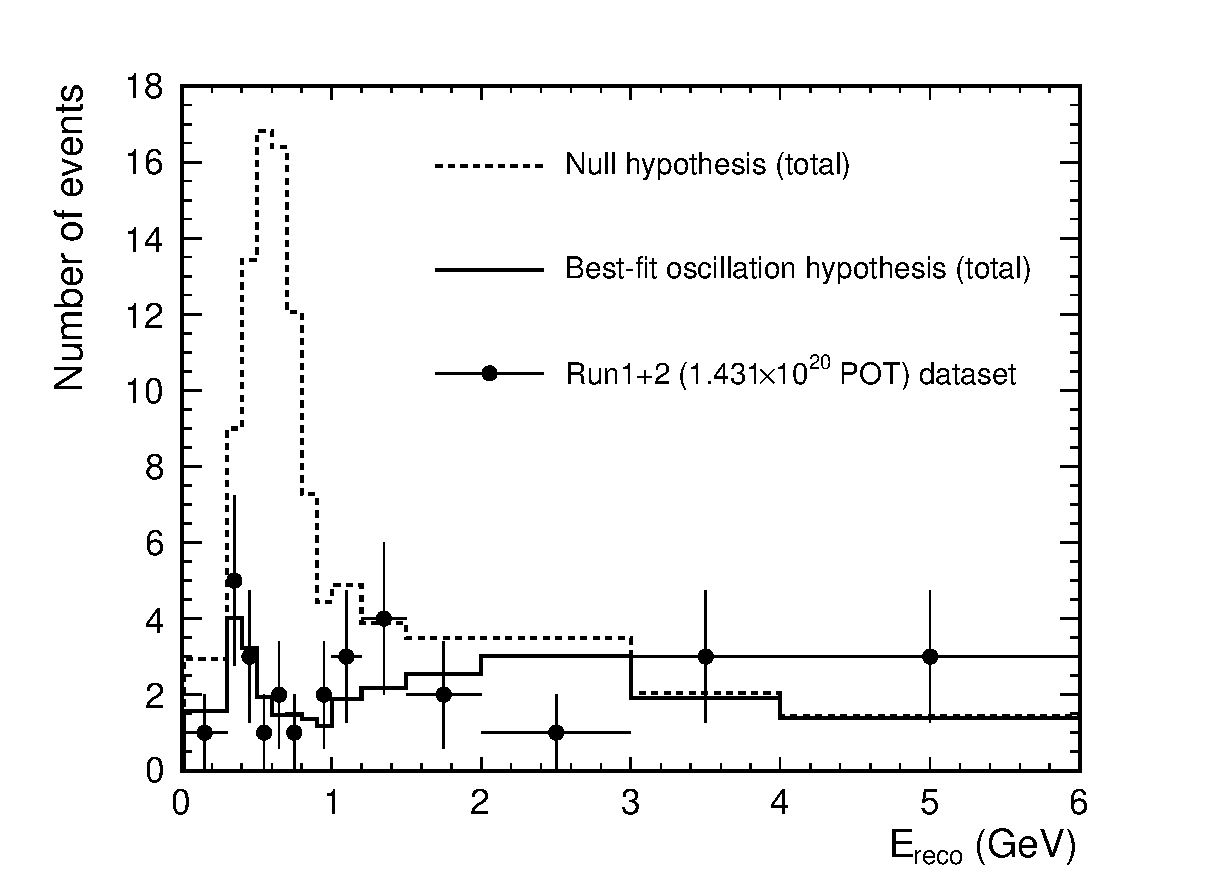
\includegraphics[width=32pc]{./images/fits/run1p2_genie_bestfit_spectrum_rebin.eps}
\caption{
  Reconstructed neutrino energy distribution of the 31 single $\mu$-like ring events of the combined
  1.431$\times$10$^{20}$ POT Run1+2 dataset (points) and GENIE best-fit SuperK prediction (solid line).
  The distributions are shown using a variable binning scheme; this is for illustration purposes only, 
  and this binning scheme was not used in the analysis.
  The best-fit oscillation parameters are
  $|\Delta m^{2}_{23}|$ = 2.60$\times$10$^{-3}$ $eV^{2}/c^{4}$ and $sin^{2}2\theta_{23}$ = 0.97.
  The dotted line shows the GENIE prediction without oscillations.
}
\label{fig:run1p2_spectrum_and_data_genie_rebin}
\end{figure*}

\begin{figure*}[htb]
\center
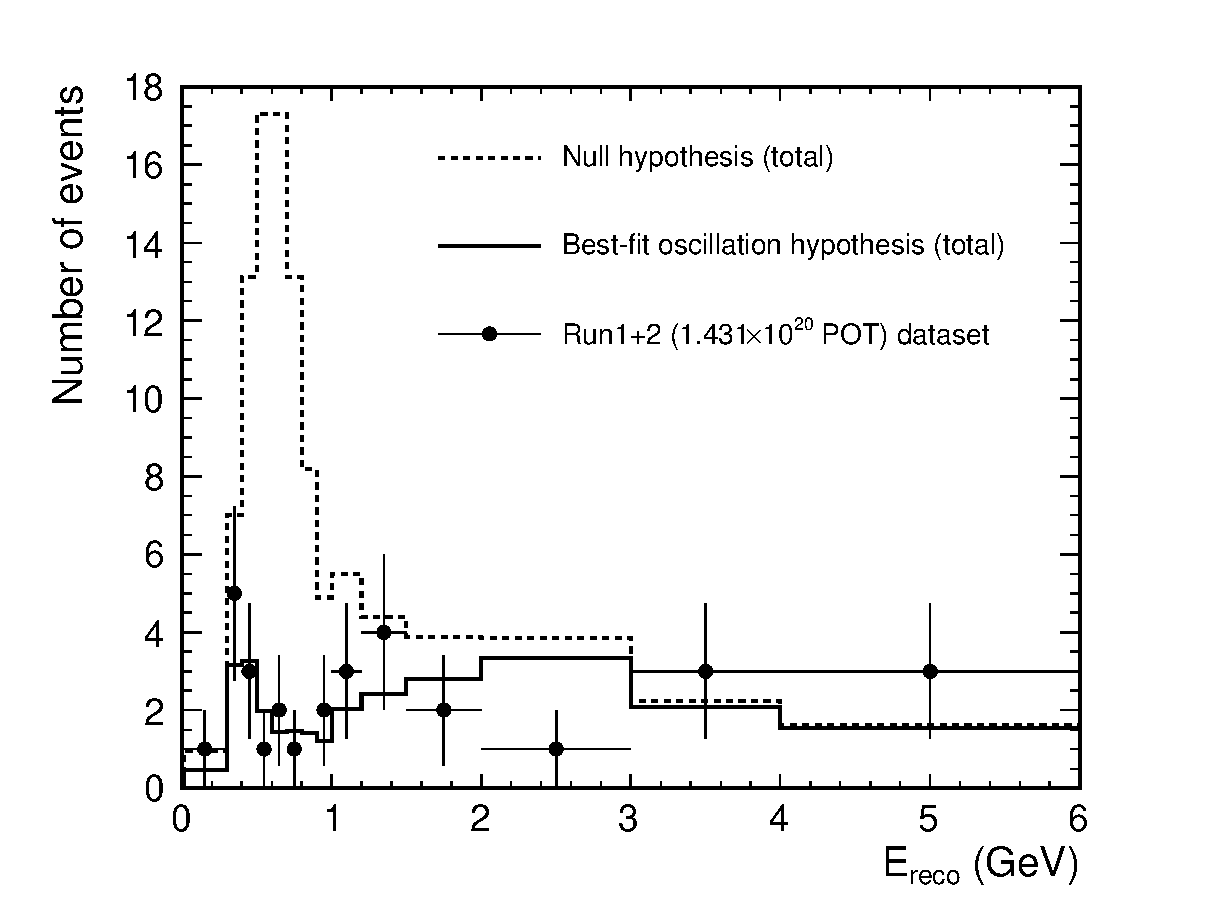
\includegraphics[width=32pc]{./images/fits/run1p2_neut_bestfit_spectrum_rebin.eps}
\caption{
  Reconstructed neutrino energy distribution of the 31 single $\mu$-like ring events of the combined
  1.431$\times$10$^{20}$ POT Run1+2 dataset (points) and NEUT best-fit SuperK prediction (solid line).
  The distributions are shown using a variable binning scheme; this is for illustration purposes only,
  and this binning scheme was not used in the analysis.
  The best-fit oscillation parameters are
  $|\Delta m^{2}_{23}|$ = 2.65$\times$10$^{-3}$ $eV^{2}/c^{4}$ and $sin^{2}2\theta_{23}$ = 0.98.
  The dotted line shows the NEUT prediction without oscillations.
}
\label{fig:run1p2_spectrum_and_data_neut_rebin}
\end{figure*}

%
% Run1+2 fit data/best-fit distribution (variable binning + CCQE/other)
%

\begin{figure*}[htb]
\center
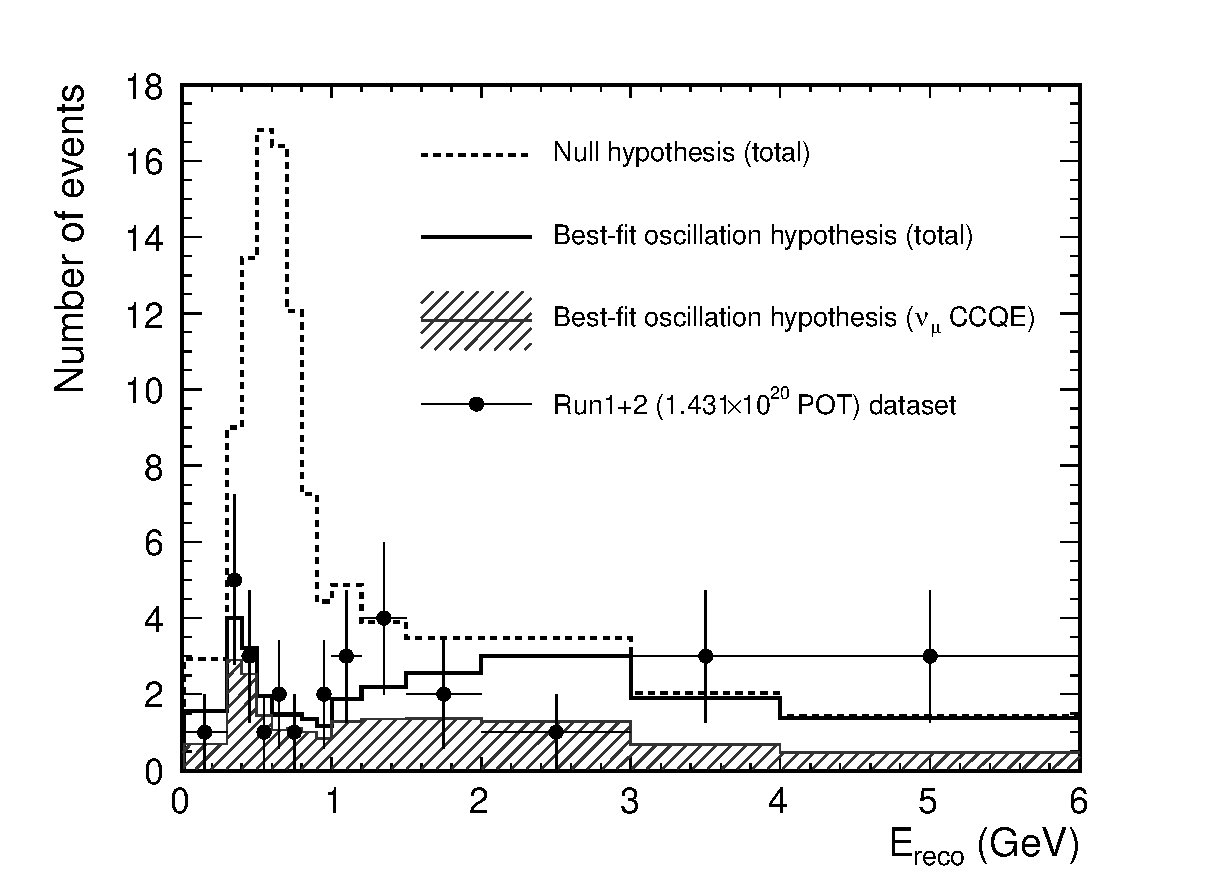
\includegraphics[width=32pc]{./images/fits/run1p2_genie_bestfit_spectrum_rebin_modes.eps}
\caption{
  Same distributions as in Fig.\ref{fig:run1p2_spectrum_and_data_genie_rebin} with the 
  addtion of the $\nu_{\mu}$-CCQE component of the best-fit oscillation hypothesis (GENIE)
}
\label{fig:run1p2_spectrum_and_data_genie_rebin_modes}
\end{figure*}

\begin{figure*}[htb]
\center
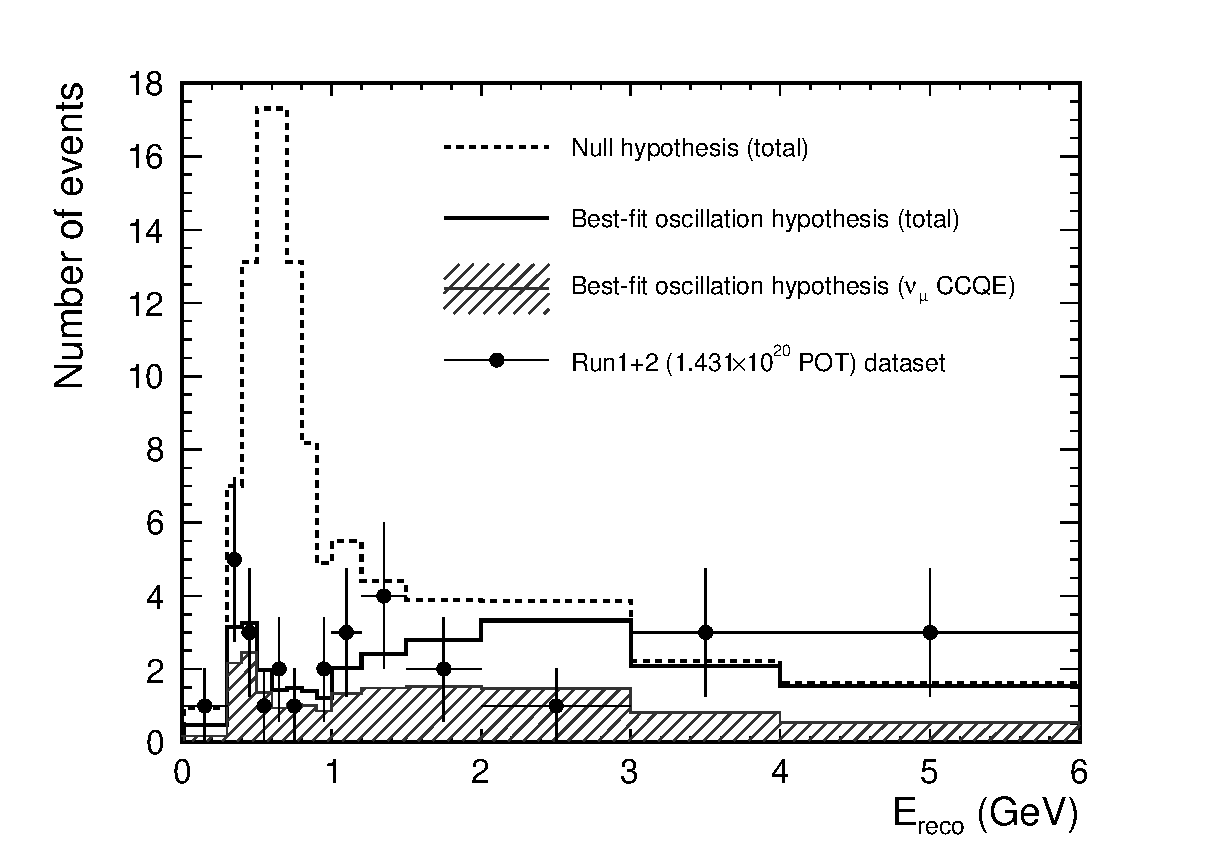
\includegraphics[width=32pc]{./images/fits/run1p2_neut_bestfit_spectrum_rebin_modes.eps}
\caption{
  Same distributions as in Fig.\ref{fig:run1p2_spectrum_and_data_neut_rebin} with the
  addition of the $\nu_{\mu}$-CCQE component of the best-fit oscillation hypothesis (NEUT)
}
\label{fig:run1p2_spectrum_and_data_neut_rebin_modes}
\end{figure*}


%
% Run1+2 delta chisq surfaces
%

\begin{figure}[ht]
\begin{minipage}[t]{0.47\linewidth}
\centering
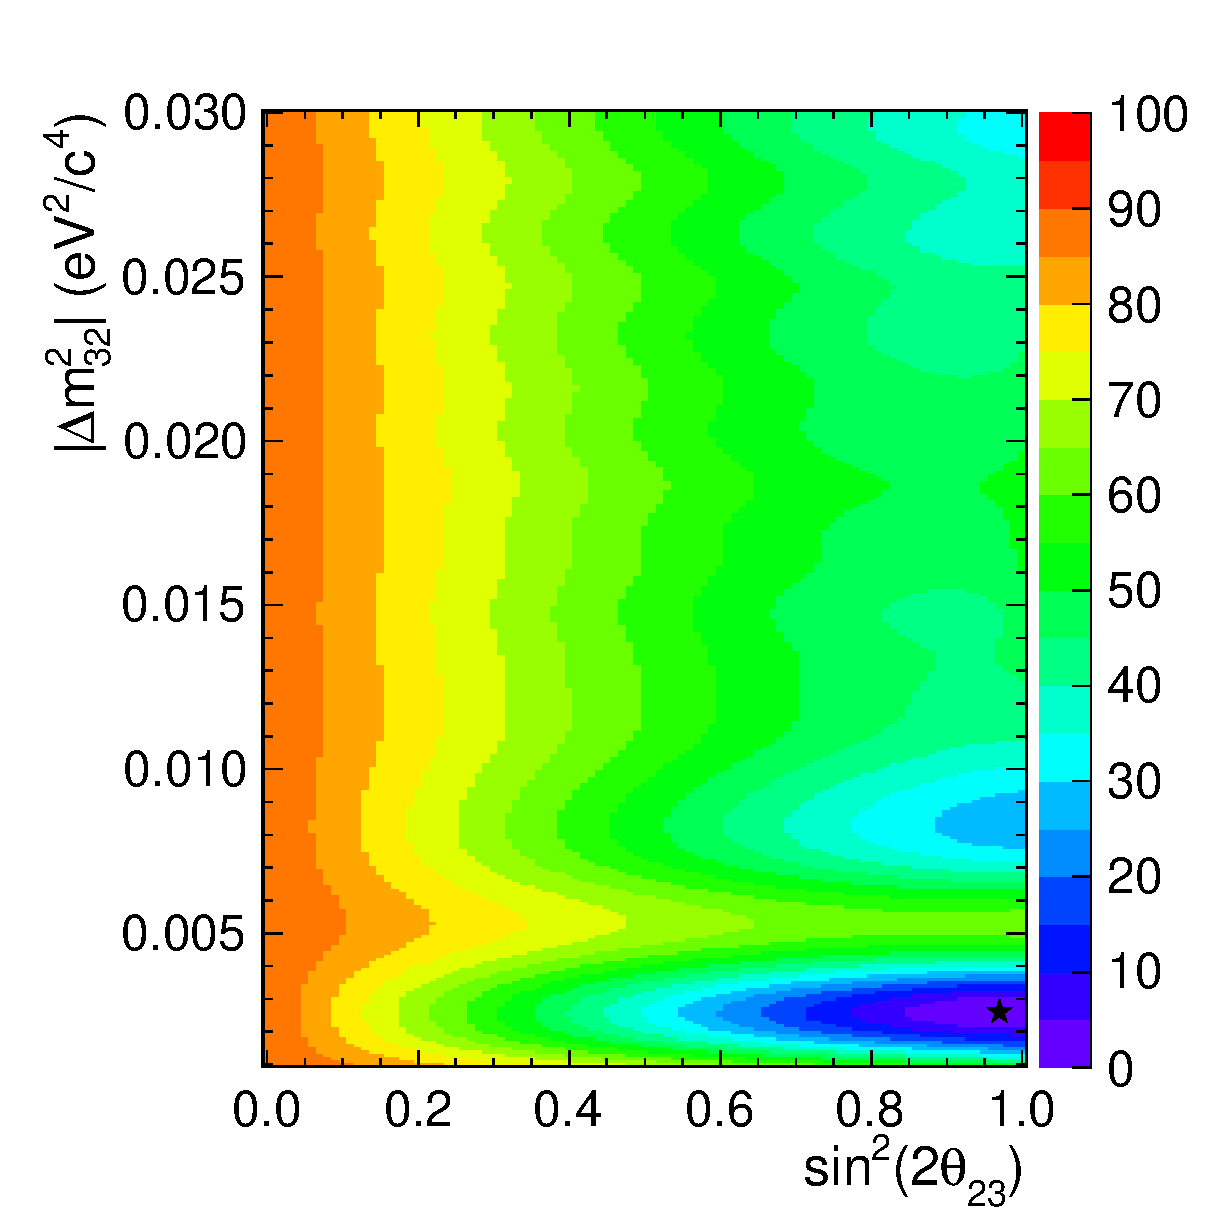
\includegraphics[width=18pc,height=19pc]{./images/fits/run1p2_genie_deltachisqsurf_wide.eps}
\caption{
  $\Delta\chi^{2}$ surface for the 2-flavour disappearance fit to the combined 1.431$\times$10$^{20}$ POT Run1+2 dataset (GENIE)
}
\label{fig:run1p2_genie_deltachisqsurf_wide}
\end{minipage}
\hspace{0.06\linewidth}
\begin{minipage}[t]{0.47\linewidth}
\centering  
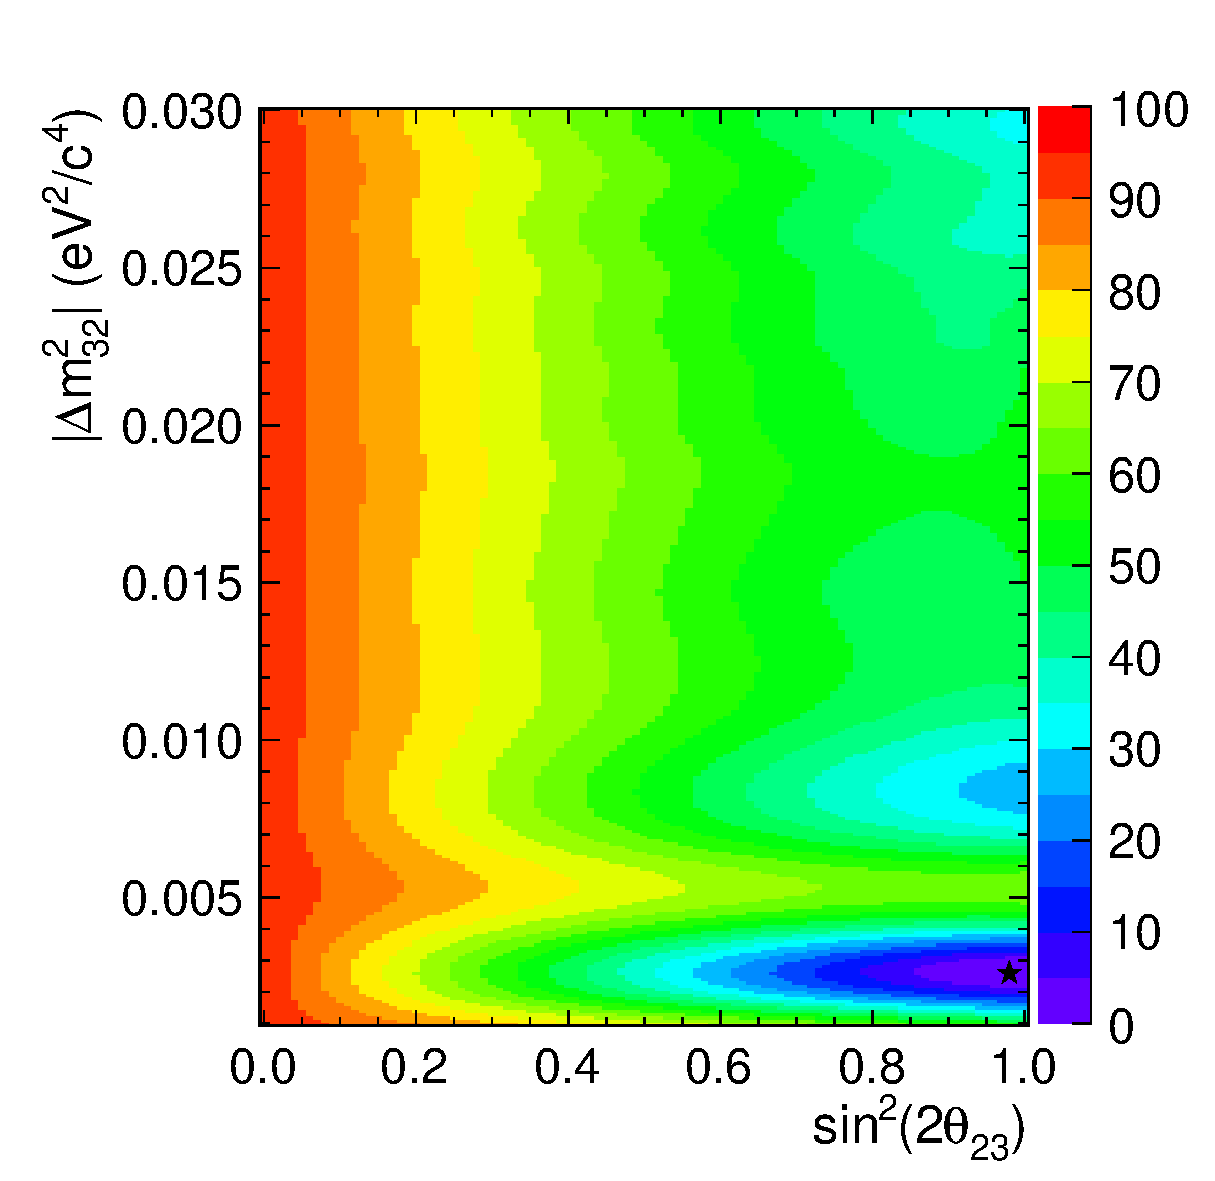
\includegraphics[width=18pc,height=19pc]{./images/fits/run1p2_neut_deltachisqsurf_wide.eps}
\caption{
  $\Delta\chi^{2}$ surface for the 2-flavour disappearance fit to the combined 1.431$\times$10$^{20}$ POT Run1+2 dataset (NEUT)
}
\label{fig:run1p2_neut_deltachisqsurf_wide}
\end{minipage}
\end{figure}

%
% Run1+2 delta chisq surfaces (zoomed around MINOS-2011 best-fit values)
%

\begin{figure}[ht]
\begin{minipage}[t]{0.47\linewidth}
\centering
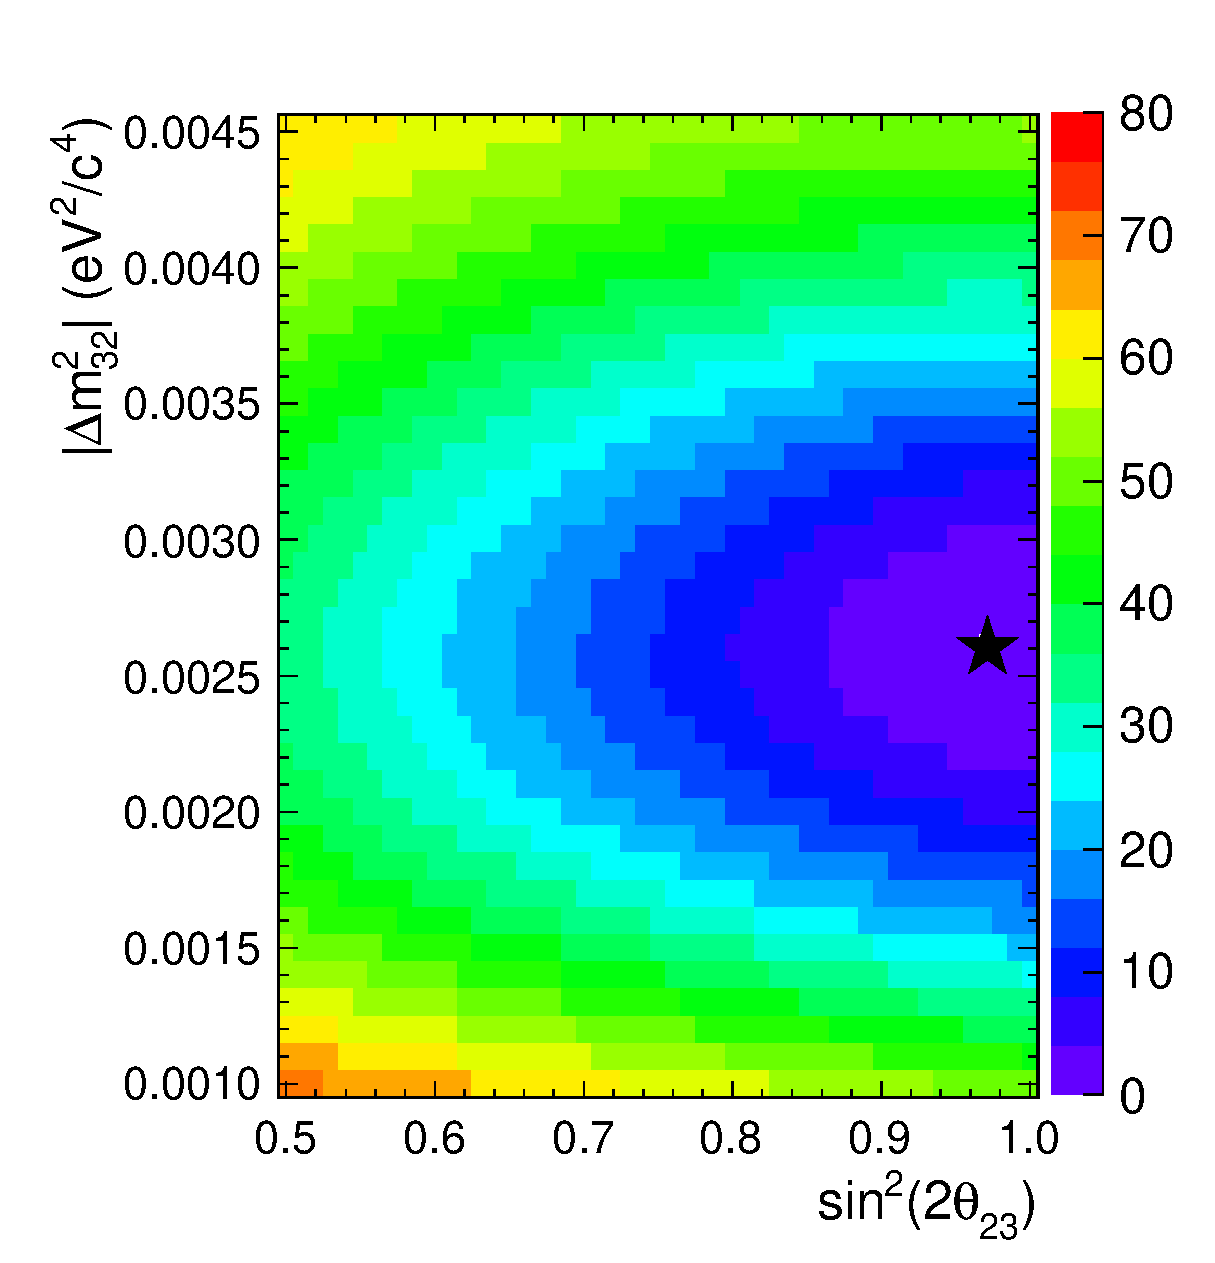
\includegraphics[width=18pc,height=19pc]{./images/fits/run1p2_genie_deltachisqsurf_zoom.eps}
\caption{
  $\Delta\chi^{2}$ surface for the 2-flavour disappearance fit to the combined 1.431$\times$10$^{20}$ POT Run1+2 dataset, 
  zoomed around the best-fit value (GENIE)
}
\label{fig:run1p2_genie_deltachisqsurf_zoom}
\end{minipage}
\hspace{0.06\linewidth}
\begin{minipage}[t]{0.47\linewidth}
\centering  
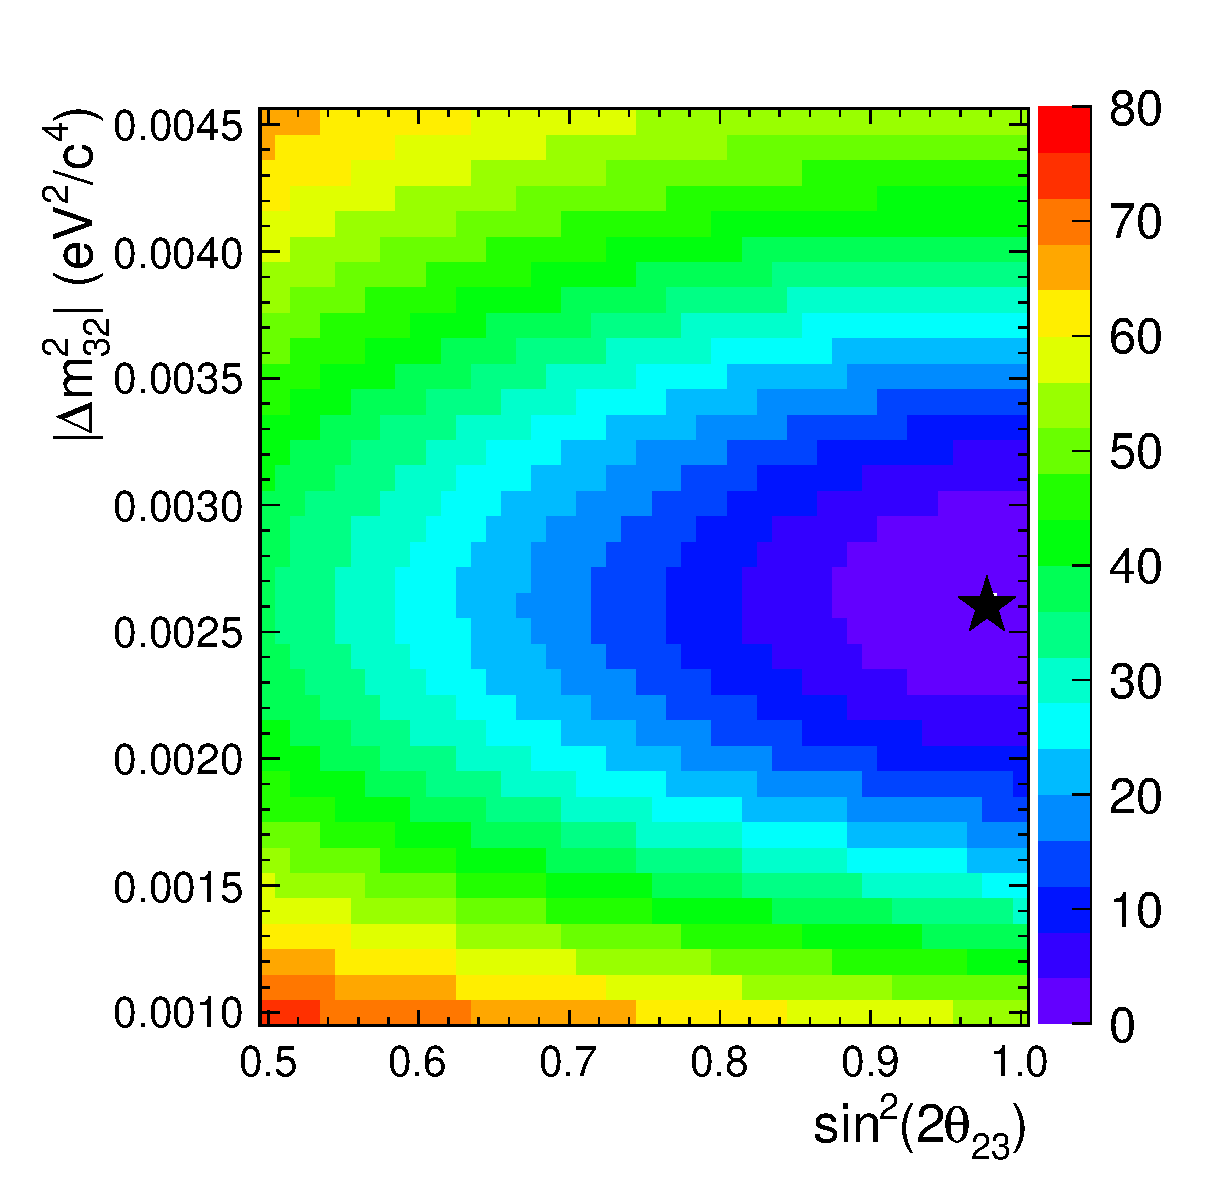
\includegraphics[width=18pc,height=19pc]{./images/fits/run1p2_neut_deltachisqsurf_zoom.eps}
\caption{
  $\Delta\chi^{2}$ surface for the 2-flavour disappearance fit to the combined 1.431$\times$10$^{20}$ POT Run1+2 dataset,
  zoomed around the best-fit value (NEUT)
}
\label{fig:run1p2_neut_deltachisqsurf_zoom}
\end{minipage}
\end{figure}

%
% Run1+2 marginalised delta chisq distributions
%

\begin{figure*}[htb]
\center
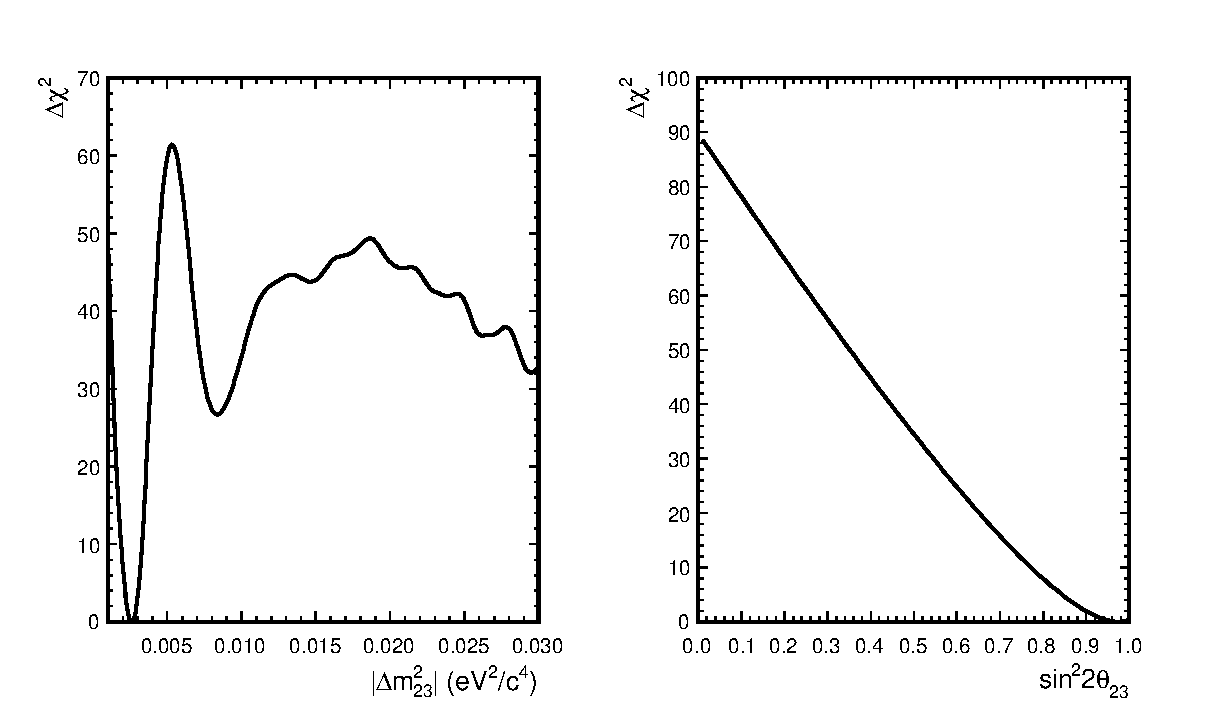
\includegraphics[width=34pc]{./images/fits/run1p2_genie_marginal_deltachisq_wide.eps}
\caption{
  Marginalised $\Delta\chi^{2}$ distributions from the 2-flavour $\nu_{\mu}$-disappearance fit 
  to the combined 1.431$\times$10$^{20}$ POT Run1+2 dataset (GENIE)
}
\label{fig:run1p2_genie_marginal_deltachisq_wide}
\end{figure*}

\begin{figure*}[htb]
\center
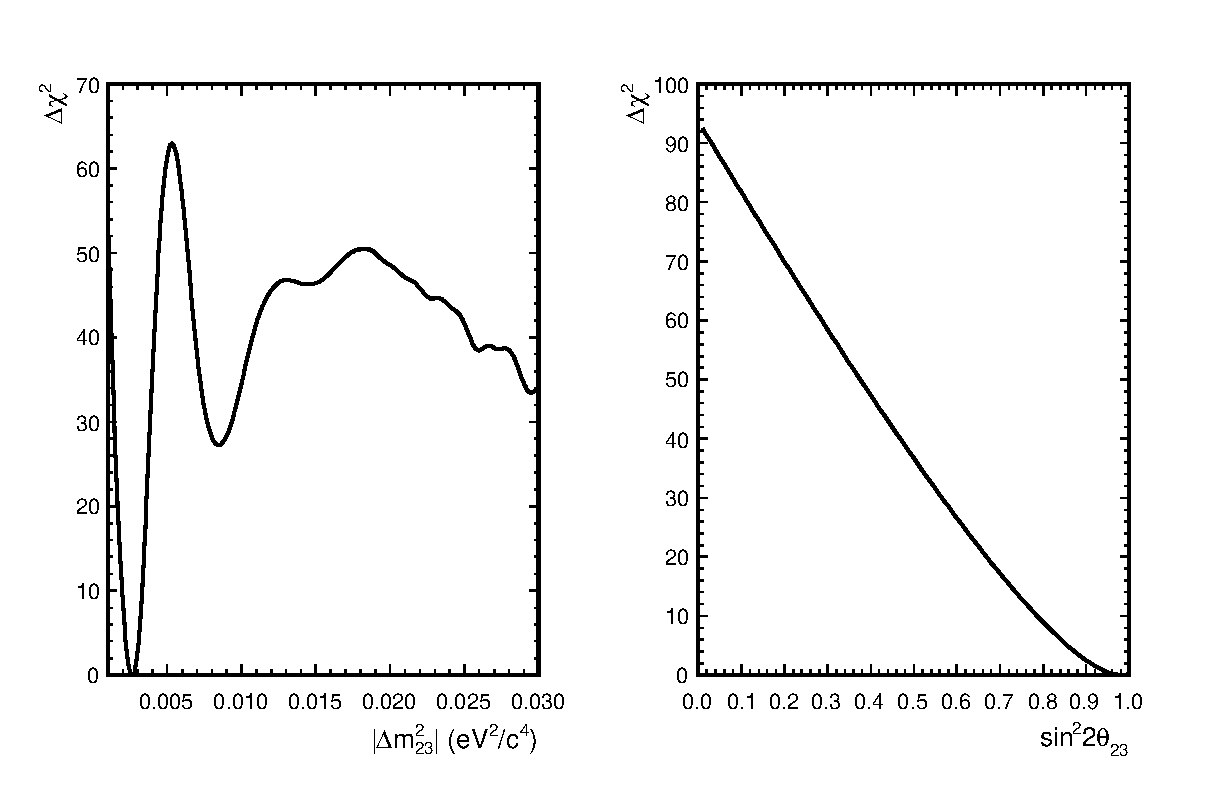
\includegraphics[width=34pc]{./images/fits/run1p2_neut_marginal_deltachisq_wide.eps}
\caption{
  Marginalised $\Delta\chi^{2}$ distributions from the 2-flavour $\nu_{\mu}$-disappearance fit 
  to the combined 1.431$\times$10$^{20}$ POT Run1+2 dataset (NEUT)
}
\label{fig:run1p2_neut_marginal_deltachisq_wide}
\end{figure*}

%
% Chisq and best-fit distributions for fits to 1.431E+20 POT toy MC expts generated with the MINOS-2011 params.
%

\begin{figure*}[ht]
\centering
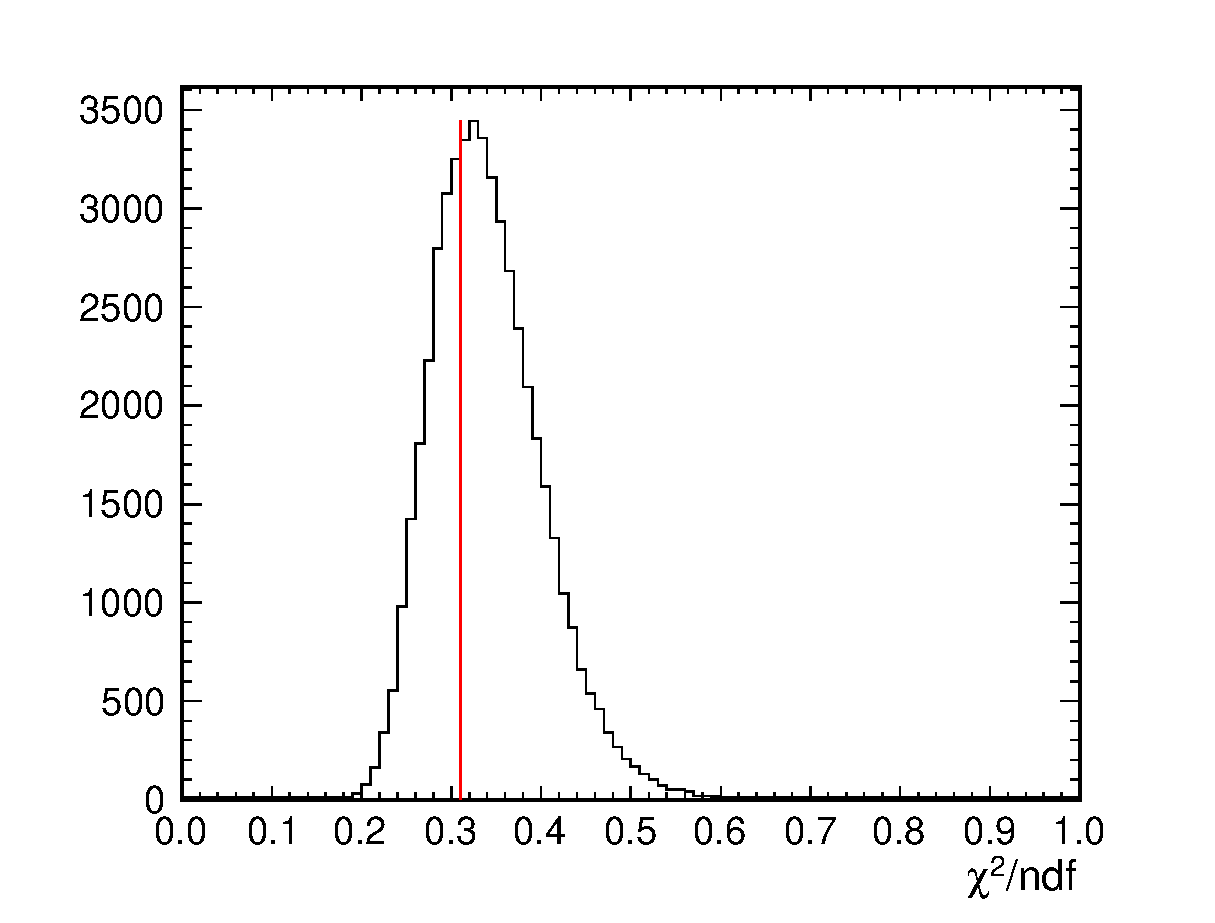
\includegraphics[height=21pc]{./images/fits/genie-minos11-run1p2-toymc-chisq-distribution.eps}
\caption{
  $chi^{2}/ndf$ distribution for fits to 1.431$\times$10$^{20}$ POT toy MC experiments 
  generated with $sin^{2}2\theta_{23}$ = 1.0 and $|\Delta m^{2}_{23}|$ = 2.32$\times10^{-3}$ $eV^{2}/c^{4}$.
  The $chi^{2}/ndf$ value for the fit to the Run1+2 dataset is also shown with a red line (GENIE).
}
\label{fig:genie-minos11-run1p2-toymc-chisq-distribution}
\end{figure*}

\begin{figure*}[ht]
\centering
\centering  
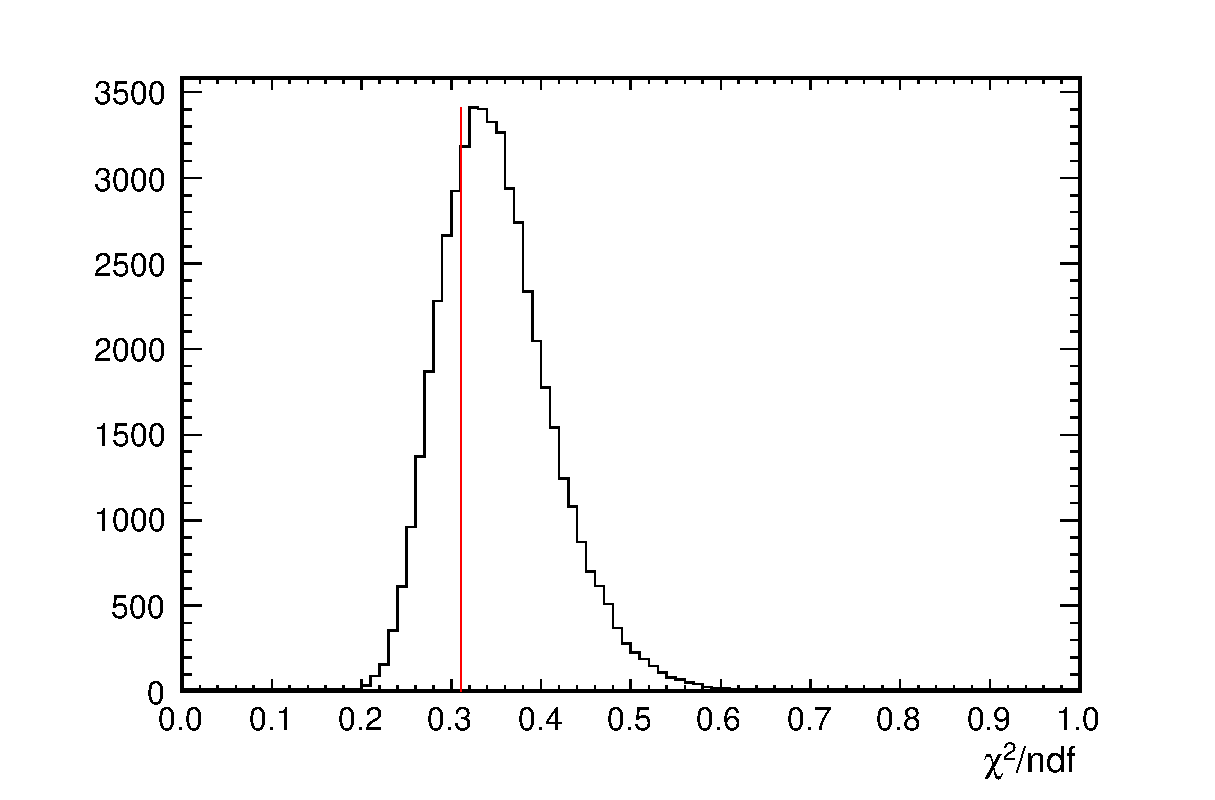
\includegraphics[height=21pc]{./images/fits/neut-minos11-run1p2-toymc-chisq-distribution.eps}
\caption{
  $chi^{2}/ndf$ distribution for fits to 1.431$\times$10$^{20}$ POT toy MC experiments 
  generated with $sin^{2}2\theta_{23}$ = 1.0 and $|\Delta m^{2}_{23}|$ = 2.32$\times10^{-3}$ $eV^{2}/c^{4}$.
  The $chi^{2}/ndf$ value for the fit to the Run1+2 dataset is also shown with a red line (NEUT).
}
\label{fig:neut-minos11-run1p2-toymc-chisq-distribution}
\end{figure*}


%\begin{figure}[ht]
%\begin{minipage}[t]{0.47\linewidth}
%\centering
%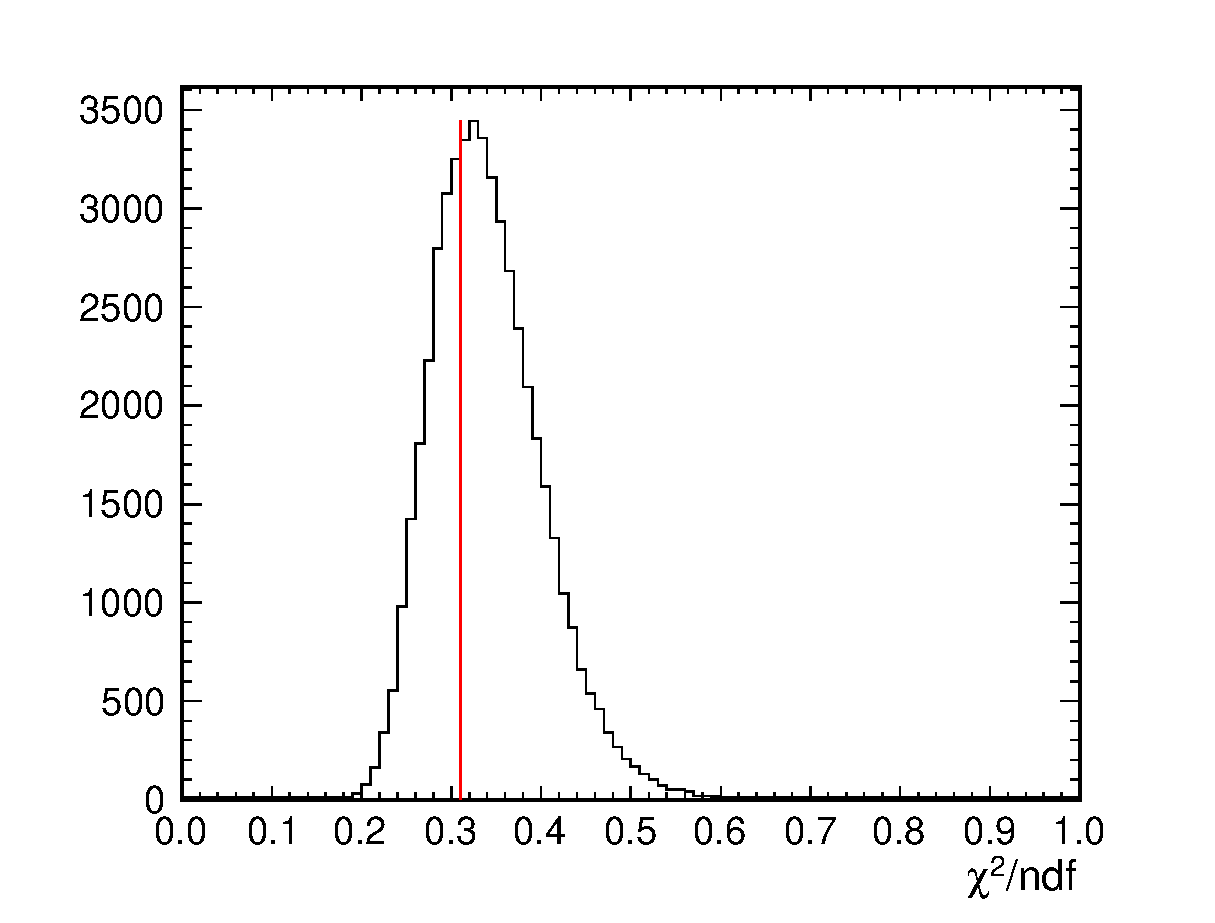
\includegraphics[width=18pc,height=19pc]{./images/fits/genie-minos11-run1p2-toymc-chisq-distribution.eps}
%\caption{
%  $chi^{2}/ndf$ distribution for fits to 1.431$\times$10$^{20}$ POT toy MC experiments 
%  generated with $sin^{2}2\theta_{23}$ = 1.0 and $|\Delta m^{2}_{23}|$ = 2.32$\times10^{-3}$ $eV^{2}/c^{4}$.
%  The $chi^{2}/ndf$ value for the fit to the Run1+2 dataset is also shown with a red line (GENIE).
%}
%\label{fig:genie-minos11-run1p2-toymc-chisq-distribution}
%\end{minipage}
%\hspace{0.06\linewidth}
%\begin{minipage}[t]{0.47\linewidth}
%\centering  
%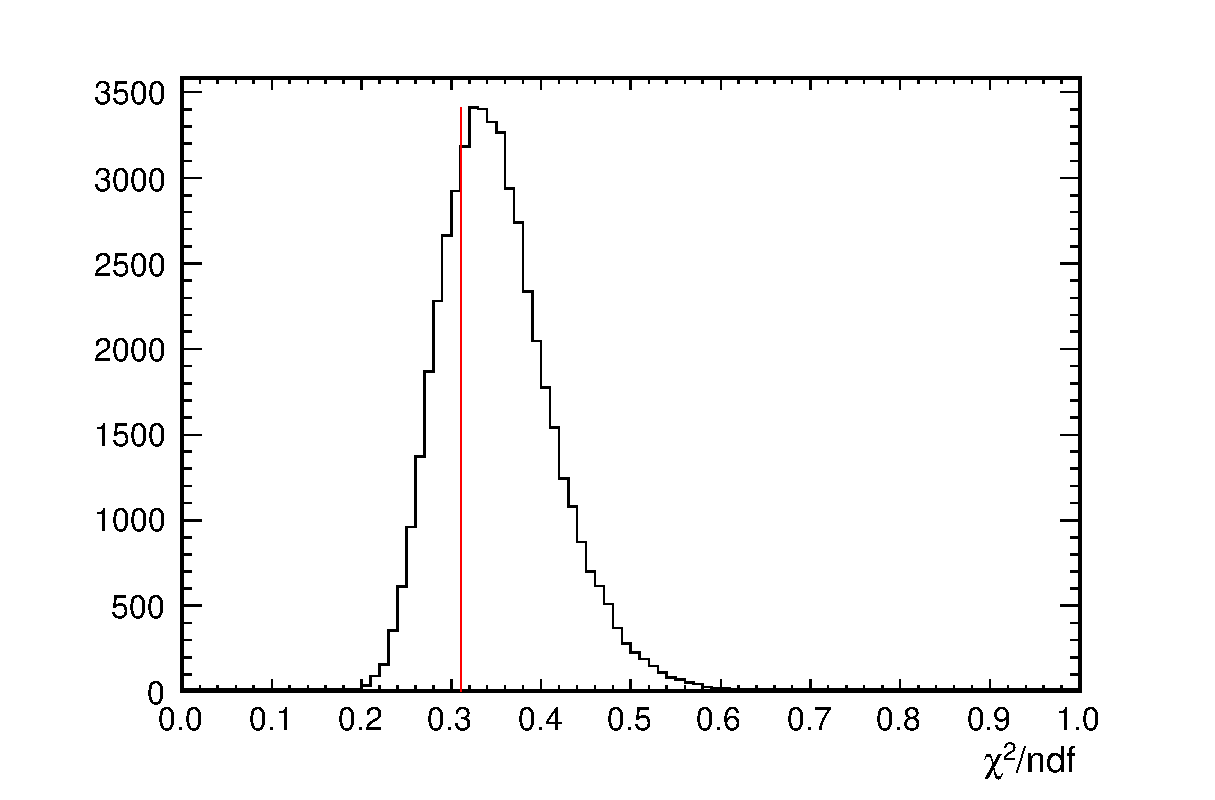
\includegraphics[width=18pc,height=19pc]{./images/fits/neut-minos11-run1p2-toymc-chisq-distribution.eps}
%\caption{
%  $chi^{2}/ndf$ distribution for fits to 1.431$\times$10$^{20}$ POT toy MC experiments 
%  generated with $sin^{2}2\theta_{23}$ = 1.0 and $|\Delta m^{2}_{23}|$ = 2.32$\times10^{-3}$ $eV^{2}/c^{4}$.
%  The $chi^{2}/ndf$ value for the fit to the Run1+2 dataset is also shown with a red line (NEUT).
%}
%\label{fig:neut-minos11-run1p2-toymc-chisq-distribution}
%\end{minipage}
%\end{figure}


\begin{figure*}[htb]
\center
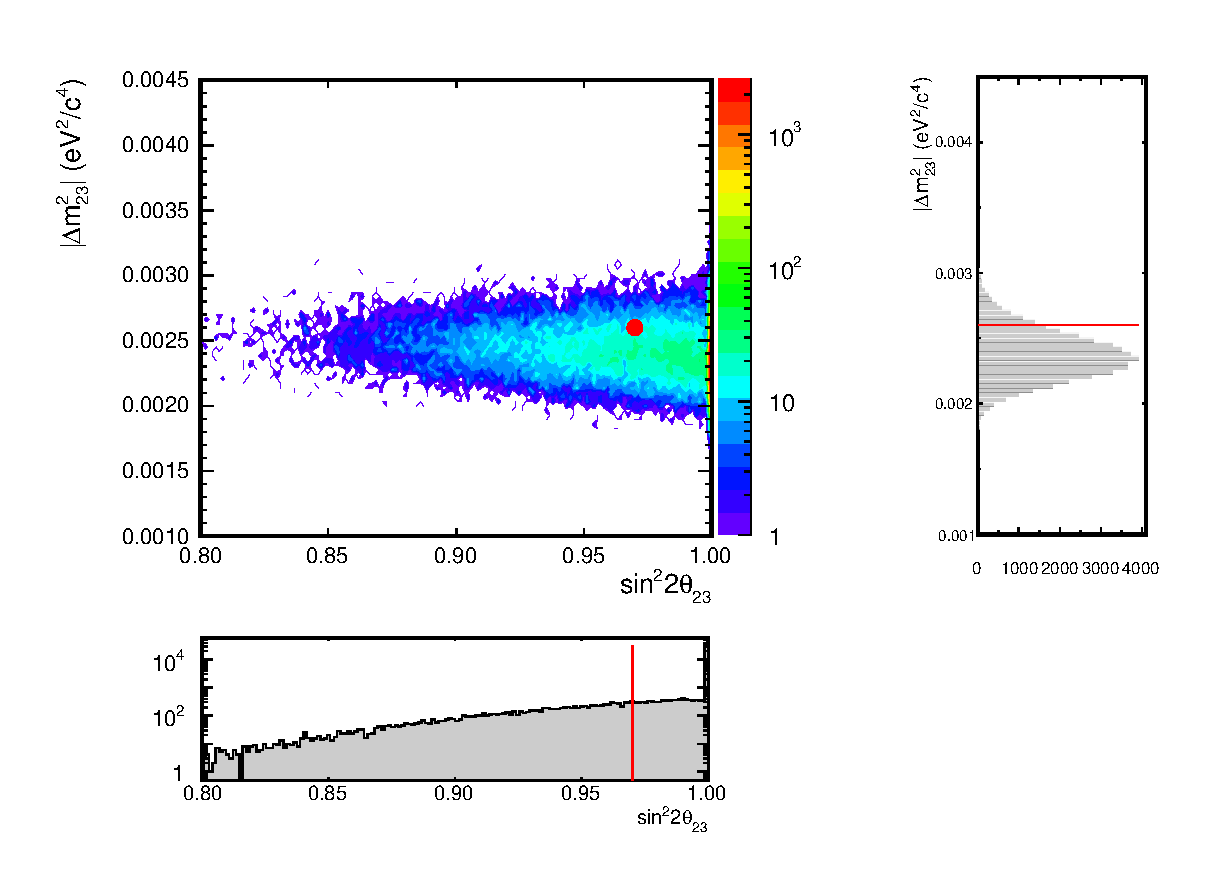
\includegraphics[width=35pc]{./images/fits/genie-minos11-run1p2-toymc-bestfitparam-distributions.eps}
\caption{
  Best-fit parameter distributions from 2-flavour $\nu_{\mu}$-disappearance 
  fits to 1.431$\times$10$^{20}$ POT toy MC experiments 
  generated with $sin^{2}2\theta_{23}$ = 1.0 and $|\Delta m^{2}_{23}|$ = 2.32$\times10^{-3}$ $eV^{2}/c^{4}$.
  The best-fit values for the fit to the Run1+2 dataset are also shown with a red marker and red lines (GENIE).
}
\label{fig:genie-minos11-run1p2-toymc-bestfitparam-distributions}
\end{figure*}

\begin{figure*}[htb]
\center
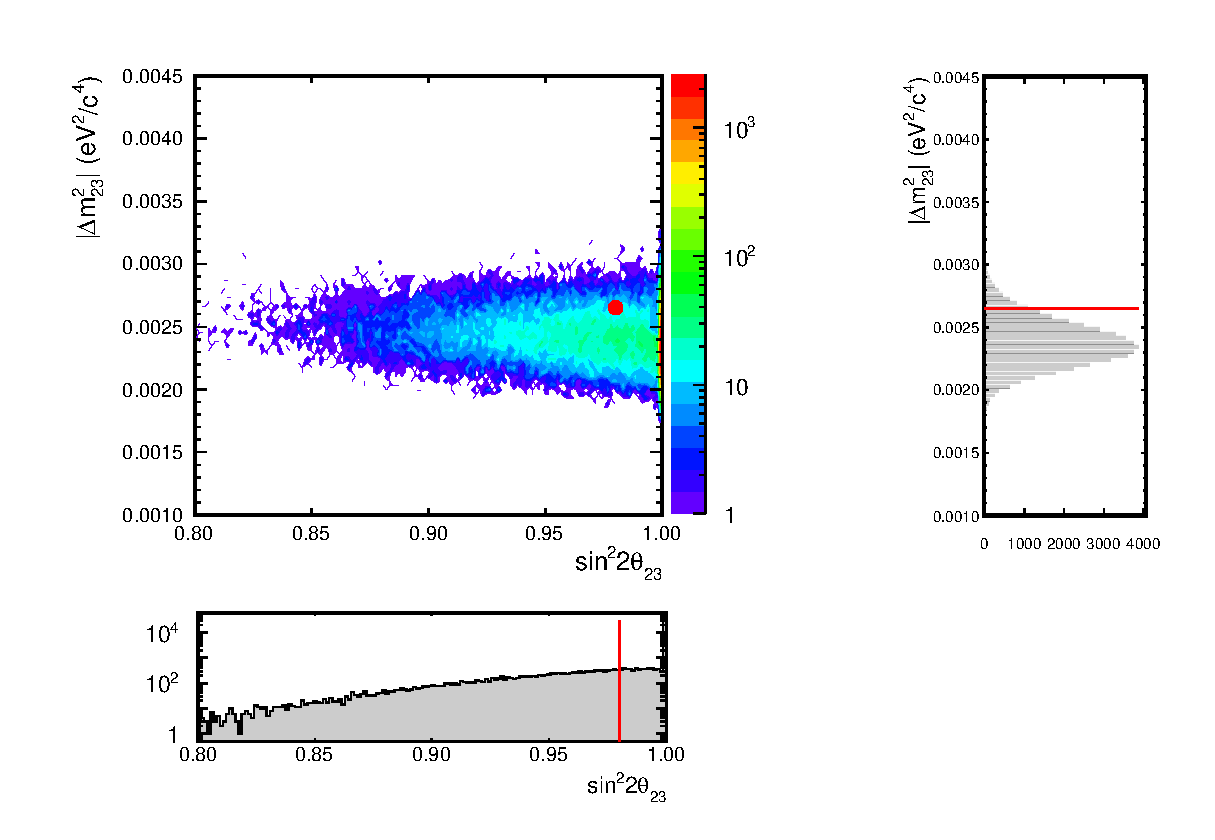
\includegraphics[width=35pc]{./images/fits/neut-minos11-run1p2-toymc-bestfitparam-distributions.eps}
\caption{
  Best-fit parameter distributions from 2-flavour $\nu_{\mu}$-disappearance 
  fits to 1.431$\times$10$^{20}$ POT toy MC experiments 
  generated with $sin^{2}2\theta_{23}$ = 1.0 and $|\Delta m^{2}_{23}|$ = 2.32$\times10^{-3}$ $eV^{2}/c^{4}$.
  The best-fit values for the fit to the Run1+2 dataset are also shown with a red marker and red lines (NEUT).
}
\label{fig:neut-minos11-run1p2-toymc-bestfitparam-distributions}
\end{figure*}

\clearpage

%
% Run1 fit data/best-fit distribution (variable binning + CCQE/other)
%

\begin{figure*}[htb]
\center
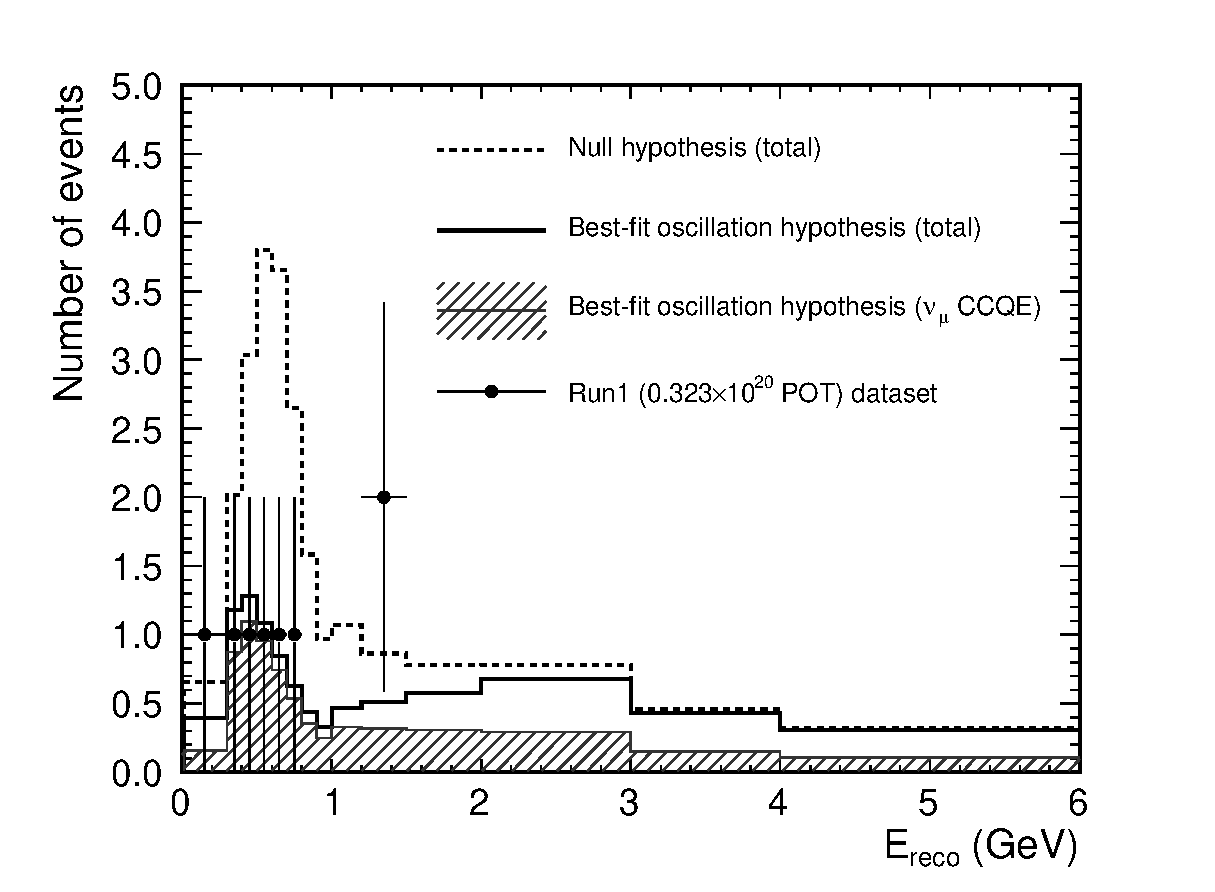
\includegraphics[height=19pc]{./images/fits/run1_genie_bestfit_spectrum_rebin_modes.eps}
\caption{
  Reconstructed neutrino energy distribution of the 8 single $\mu$-like ring events of the
  0.323$\times$10$^{20}$ POT Run1 dataset (points) and GENIE best-fit SuperK prediction (solid line).
  The best-fit oscillation parameters are
  $|\Delta m^{2}_{23}|$ = 2.77$\times$10$^{-3}$ $eV^{2}/c^{4}$ and $sin^{2}2\theta_{23}$ = 0.81
  (local minimum in first oscillation maximum region).
  The dotted line shows the GENIE prediction without oscillations.
  The distributions are not shown with 50 MeV bins as used in the oscillation fit,
  but with fewer, variable-size bins for illustration purposes.
}
\label{fig:run1_spectrum_and_data_genie_rebin_modes}
\end{figure*}

\begin{figure*}[htb]
\center
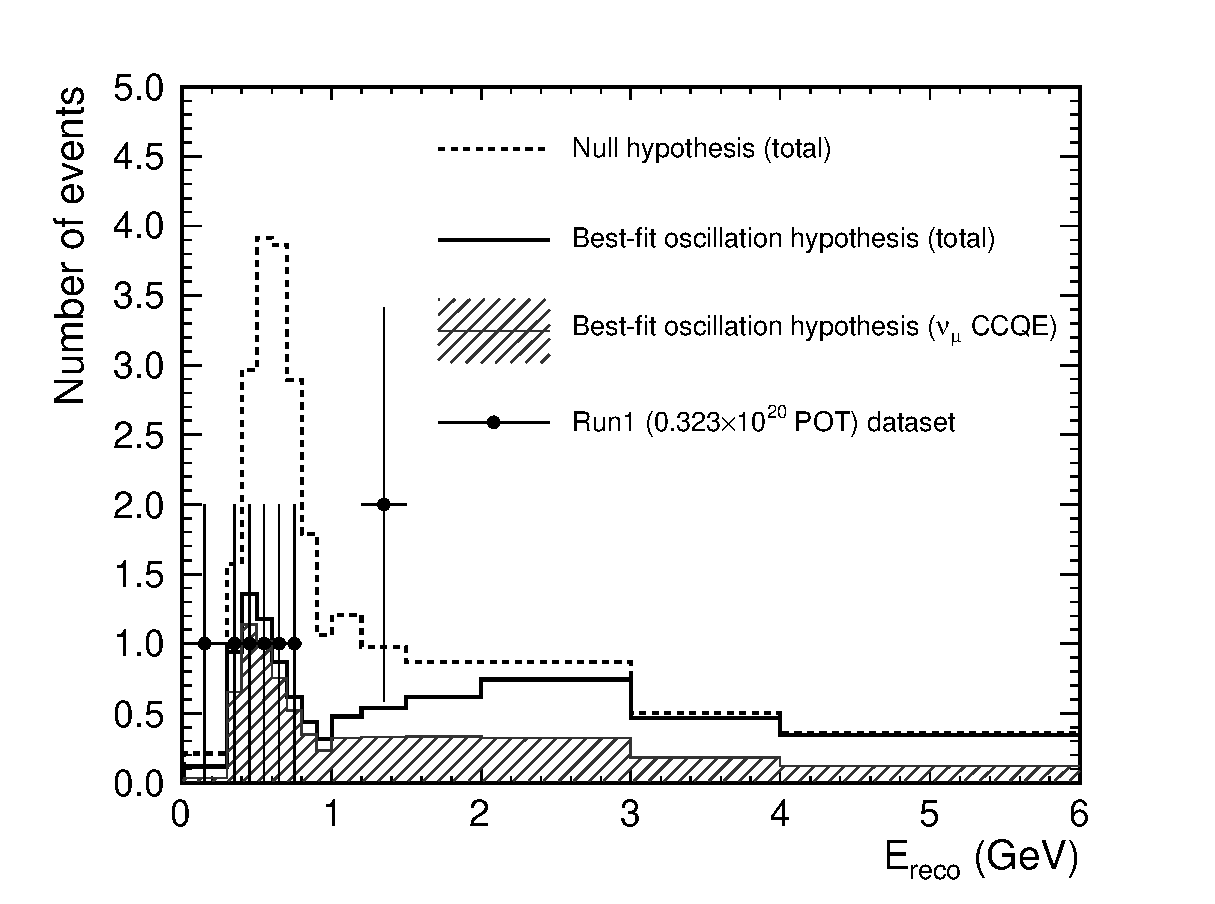
\includegraphics[height=19pc]{./images/fits/run1_neut_bestfit_spectrum_rebin_modes.eps}
\caption{
  Reconstructed neutrino energy distribution of the 8 single $\mu$-like ring events of the
  0.323$\times$10$^{20}$ POT Run1 dataset (points) and NEUT best-fit SuperK prediction (solid line).
  The best-fit oscillation parameters are
  $|\Delta m^{2}_{23}|$ = 2.88$\times$10$^{-3}$ $eV^{2}/c^{4}$ and $sin^{2}2\theta_{23}$ = 0.84
  (local minimum in first oscillation maximum region).
  The dotted line shows the NEUT prediction without oscillations.
  The distributions are not shown with 50 MeV bins as used in the oscillation fit,
  but with fewer, variable-size bins for illustration purposes.
}
\label{fig:run1_spectrum_and_data_neut_rebin_modes}
\end{figure*}


%
% Run2 fit data/best-fit distribution (variable binning + CCQE/other)
%

\begin{figure*}[htb]
\center
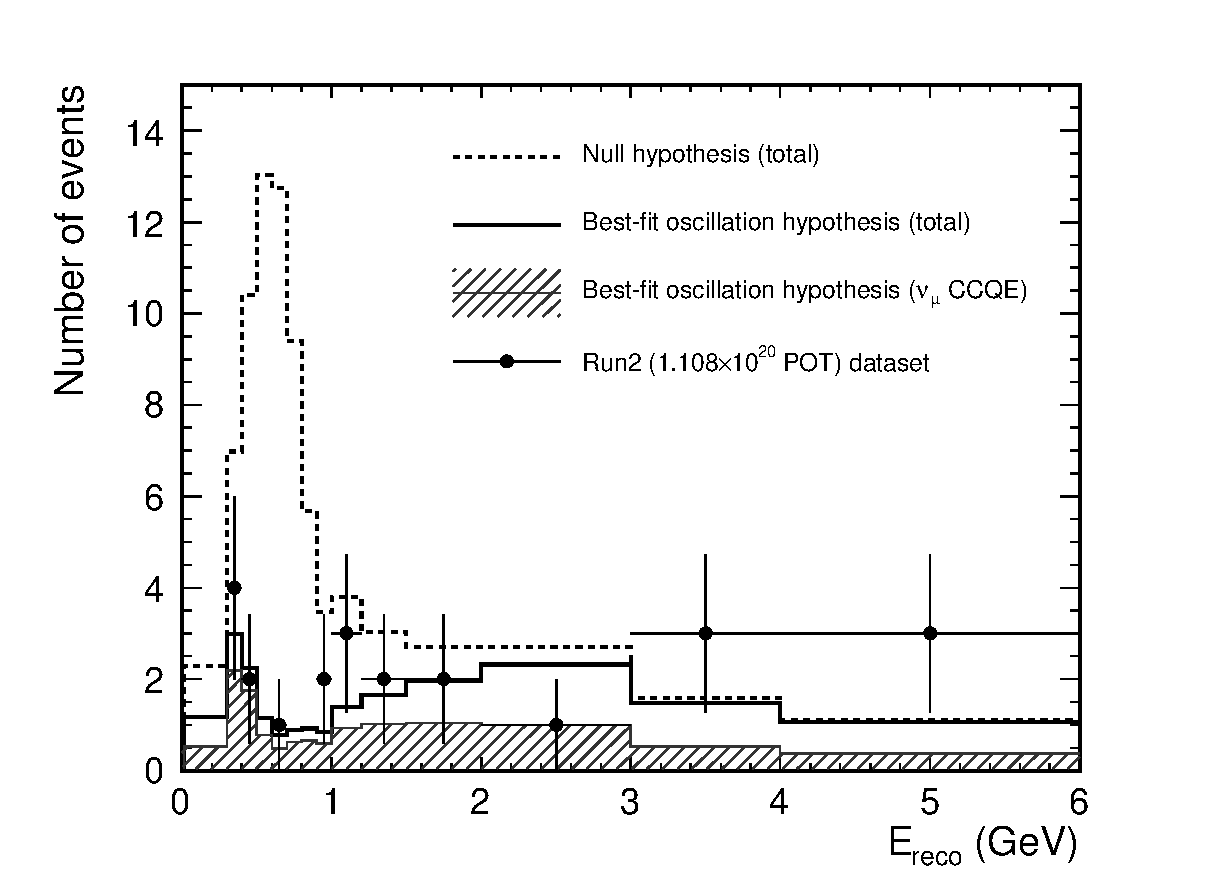
\includegraphics[width=32pc]{./images/fits/run2_genie_bestfit_spectrum_rebin_modes.eps}
\caption{
  Reconstructed neutrino energy distribution of the 23 single $\mu$-like ring events of the
  1.108$\times$10$^{20}$ POT Run2 dataset (points) and GENIE best-fit SuperK prediction (solid line).
  The best-fit oscillation parameters are
  $|\Delta m^{2}_{23}|$ = 2.59$\times$10$^{-3}$ $eV^{2}/c^{4}$ and $sin^{2}2\theta_{23}$ = 1.00.
  The dotted line shows the GENIE prediction without oscillations.
  The distributions are not shown with 50 MeV bins as used in the oscillation fit,
  but with fewer, variable-size bins for illustration purposes.
}
\label{fig:run2_spectrum_and_data_genie_rebin_modes}
\end{figure*}

\begin{figure*}[htb]
\center
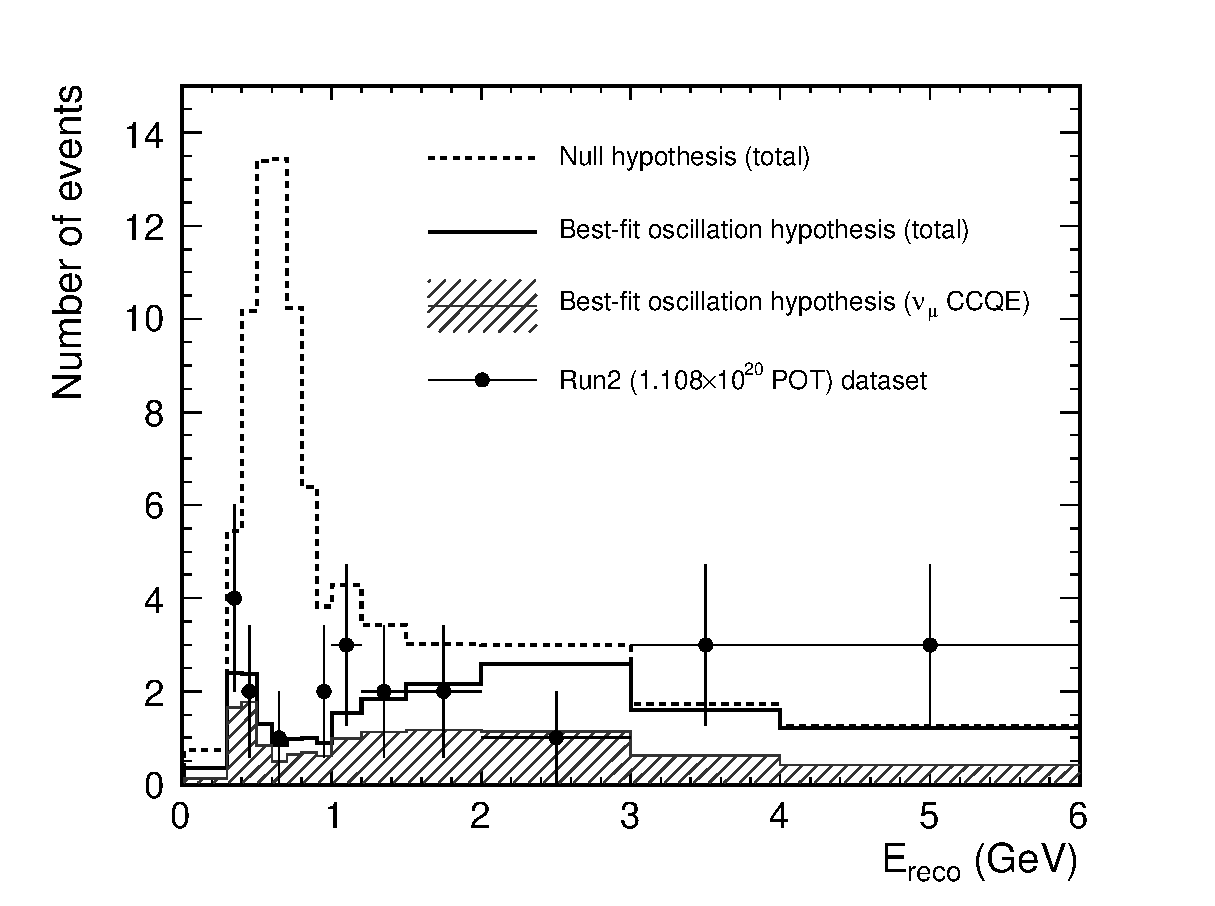
\includegraphics[width=32pc]{./images/fits/run2_neut_bestfit_spectrum_rebin_modes.eps}
\caption{
  Reconstructed neutrino energy distribution of the 23 single $\mu$-like ring events of the
  1.108$\times$10$^{20}$ POT Run2 dataset (points) and NEUT best-fit SuperK prediction (solid line).
  The best-fit oscillation parameters are
  $|\Delta m^{2}_{23}|$ = 2.62$\times$10$^{-3}$ $eV^{2}/c^{4}$ and $sin^{2}2\theta_{23}$ = 1.00.
  The dotted line shows the NEUT prediction without oscillations.
  The distributions are not shown with 50 MeV bins as used in the oscillation fit,
  but with fewer, variable-size bins for illustration purposes.
}
\label{fig:run2_spectrum_and_data_neut_rebin_modes}
\end{figure*}


%
% Run1, Run2 and Run1+2 marginalised chisq distributions
%

% dmsq (restricted)
\begin{figure}[ht]
\begin{minipage}[t]{0.47\linewidth}
\centering
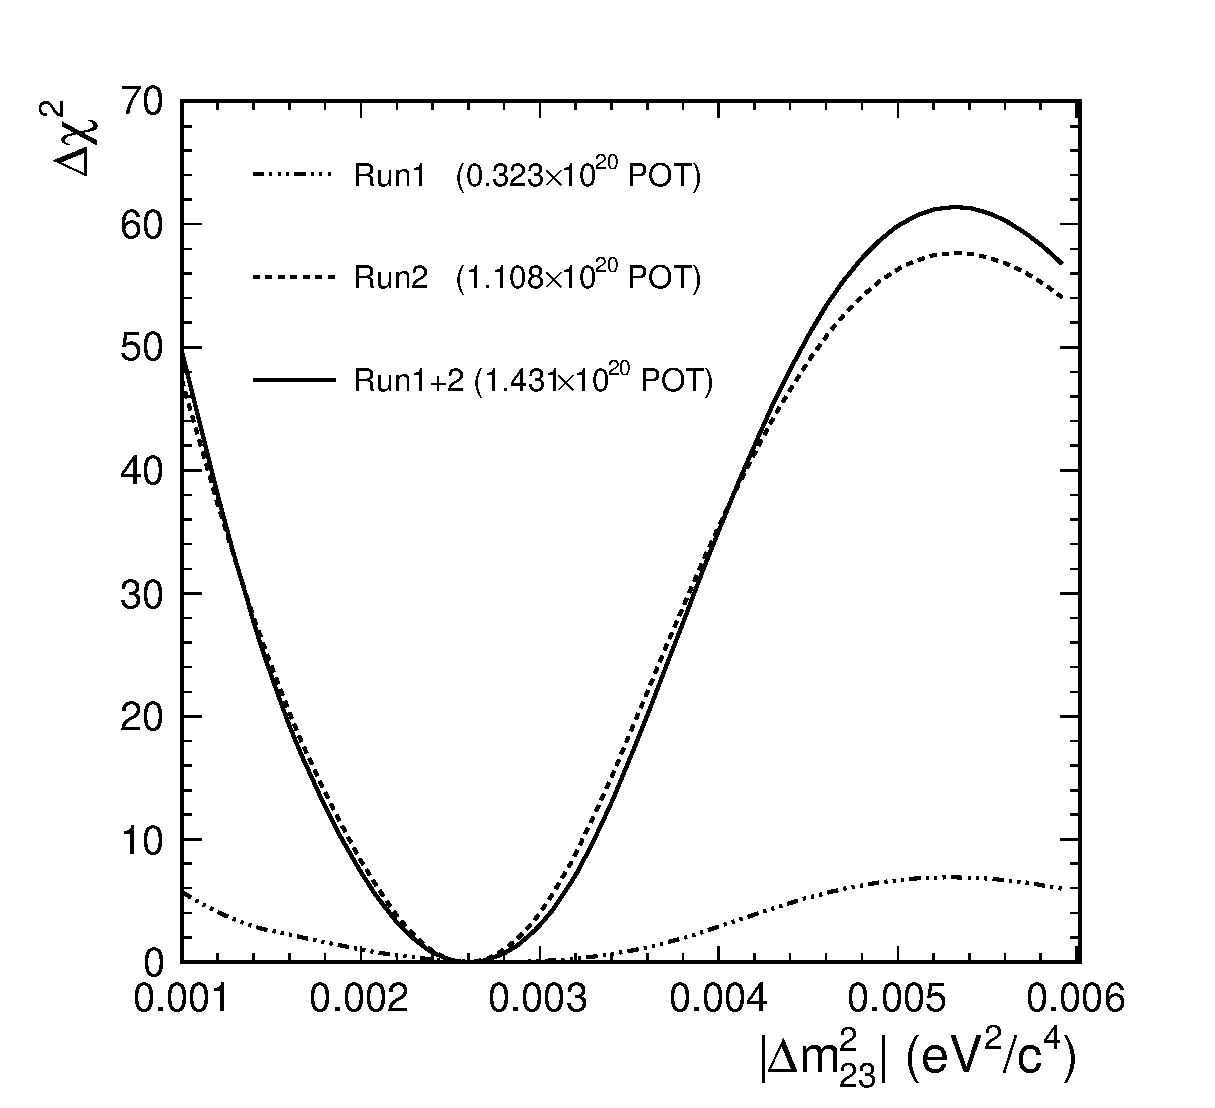
\includegraphics[width=18pc,height=19pc]{./images/fits/genie_marginal_deltachisq_dmsq_narrow_3datasets.eps}
\caption{
  The marginalised $\Delta\chi^{2}$ distributions as a function of $|\Delta m^{2}_{23}|$ from the 2-flavour
  $\nu_{\mu}$-disappearance fits to the Run1, Run2 and Run1+2 datasets (GENIE).
  All fits were performed in the restricted $|\Delta m^{2}_{23}|$ range from
  1$\times$10$^{-3}$ $eV^{2}/c^{4}$ to 6$\times$10$^{-3}$ $eV^{2}/c^{4}$.
}
\label{fig:genie_deltachisq_dmsq_narrow_3datasets}
\end{minipage}
\hspace{0.06\linewidth}
\begin{minipage}[t]{0.47\linewidth}
\centering  
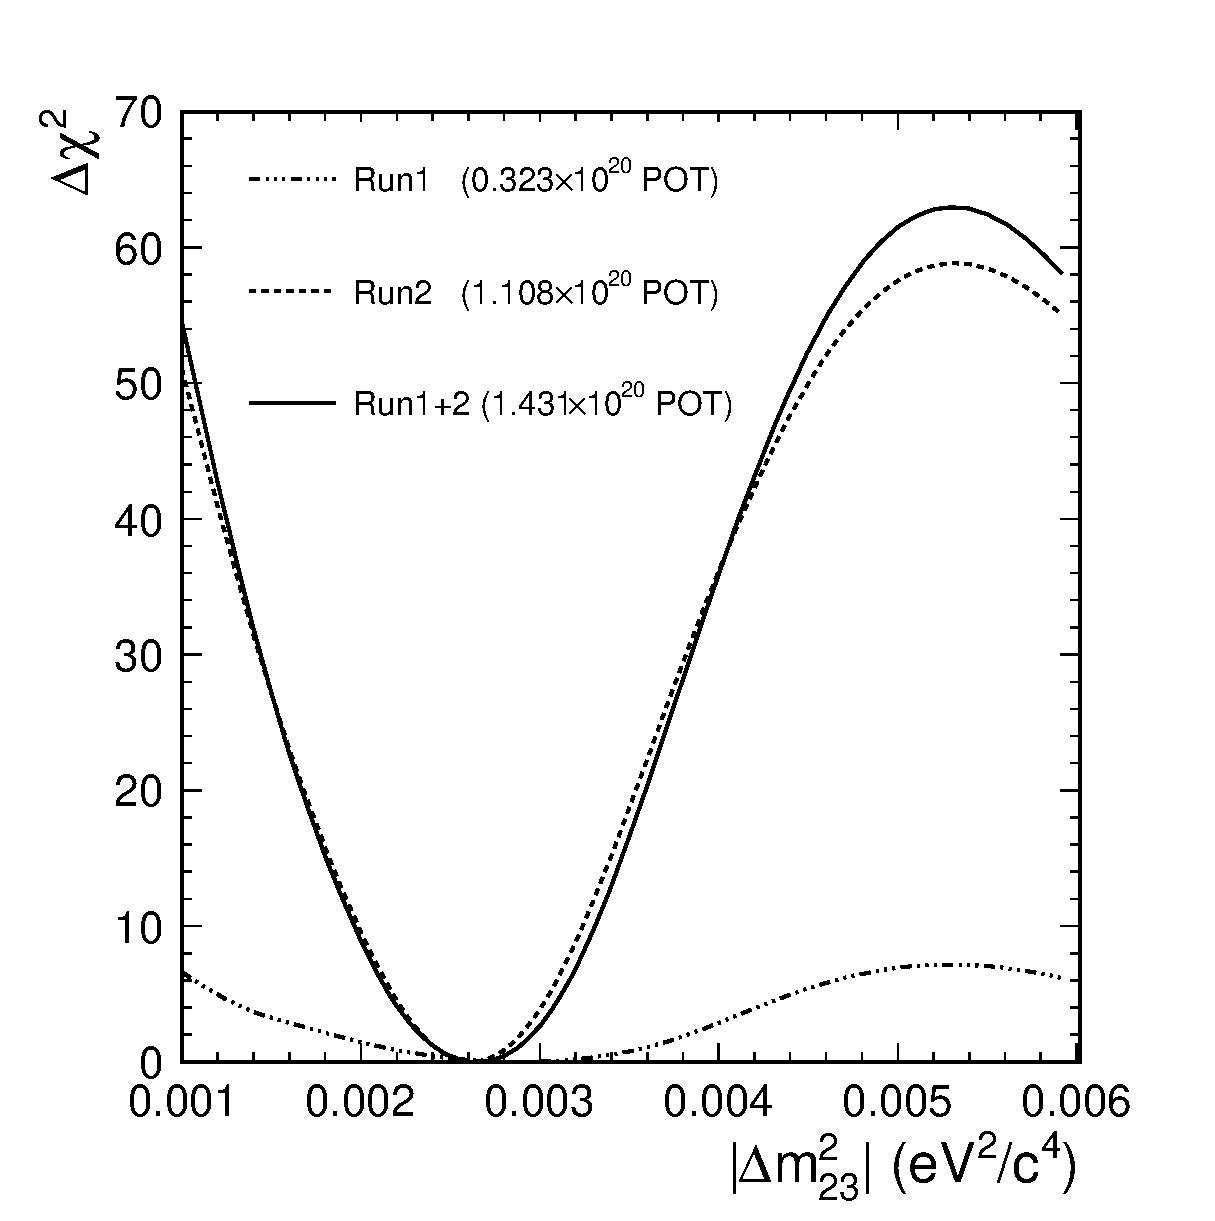
\includegraphics[width=18pc,height=19pc]{./images/fits/neut_marginal_deltachisq_dmsq_narrow_3datasets.eps}
\caption{
  The marginalised $\Delta\chi^{2}$ distributions as a function of $|\Delta m^{2}_{23}|$ from the 2-flavour
  $\nu_{\mu}$-disappearance fits to the Run1, Run2 and Run1+2 datasets (NEUT).
  All fits were performed in the restricted $|\Delta m^{2}_{23}|$ range from
  1$\times$10$^{-3}$ $eV^{2}/c^{4}$ to 6$\times$10$^{-3}$ $eV^{2}/c^{4}$.
}
\label{fig:neut_deltachisq_dmsq_narrow_3datasets}
\end{minipage}
\end{figure}

% dmsq (wide)
\begin{figure}[ht]
\begin{minipage}[t]{0.47\linewidth}
\centering
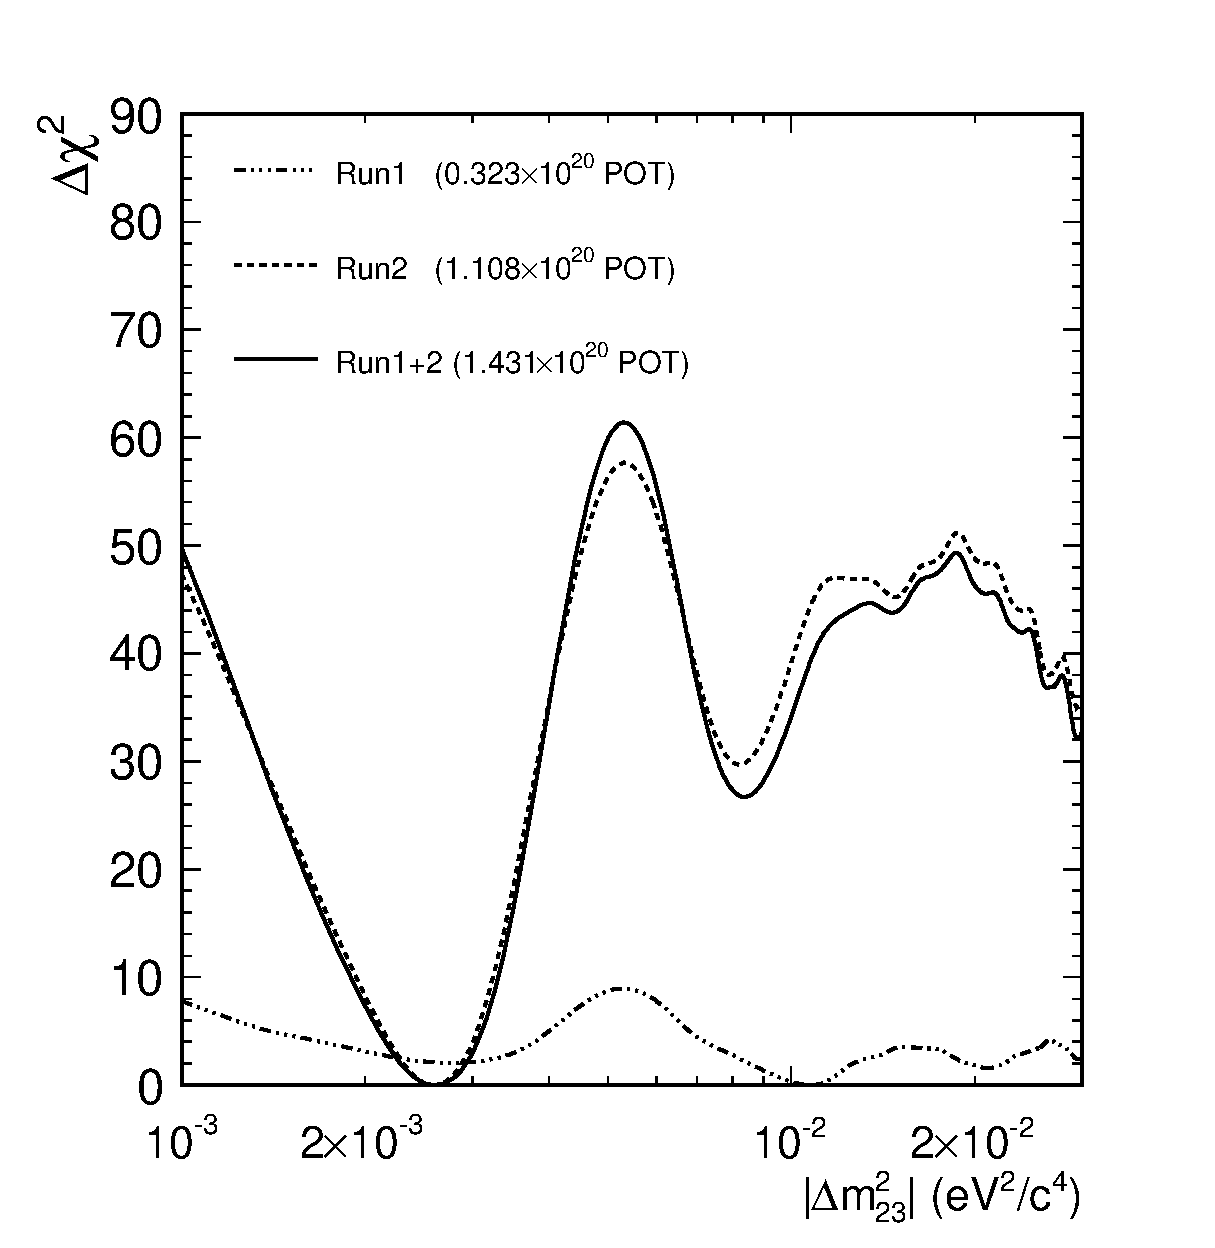
\includegraphics[width=18pc,height=19pc]{./images/fits/genie_marginal_deltachisq_dmsq_wide_3datasets.eps}
\caption{
  The marginalised $\Delta\chi^{2}$ distributions as a function of $|\Delta m^{2}_{23}|$ from the 2-flavour
  $\nu_{\mu}$-disappearance fits to the Run1, Run2 and Run1+2 datasets (GENIE).
  All fits were performed in the extended $|\Delta m^{2}_{23}|$ range from 
  1$\times$10$^{-3}$ $eV^{2}/c^{4}$ to 30$\times$10$^{-3}$ $eV^{2}/c^{4}$.
}
\label{fig:genie_deltachisq_dmsq_wide_3datasets}
\end{minipage}
\hspace{0.06\linewidth}
\begin{minipage}[t]{0.47\linewidth}
\centering  
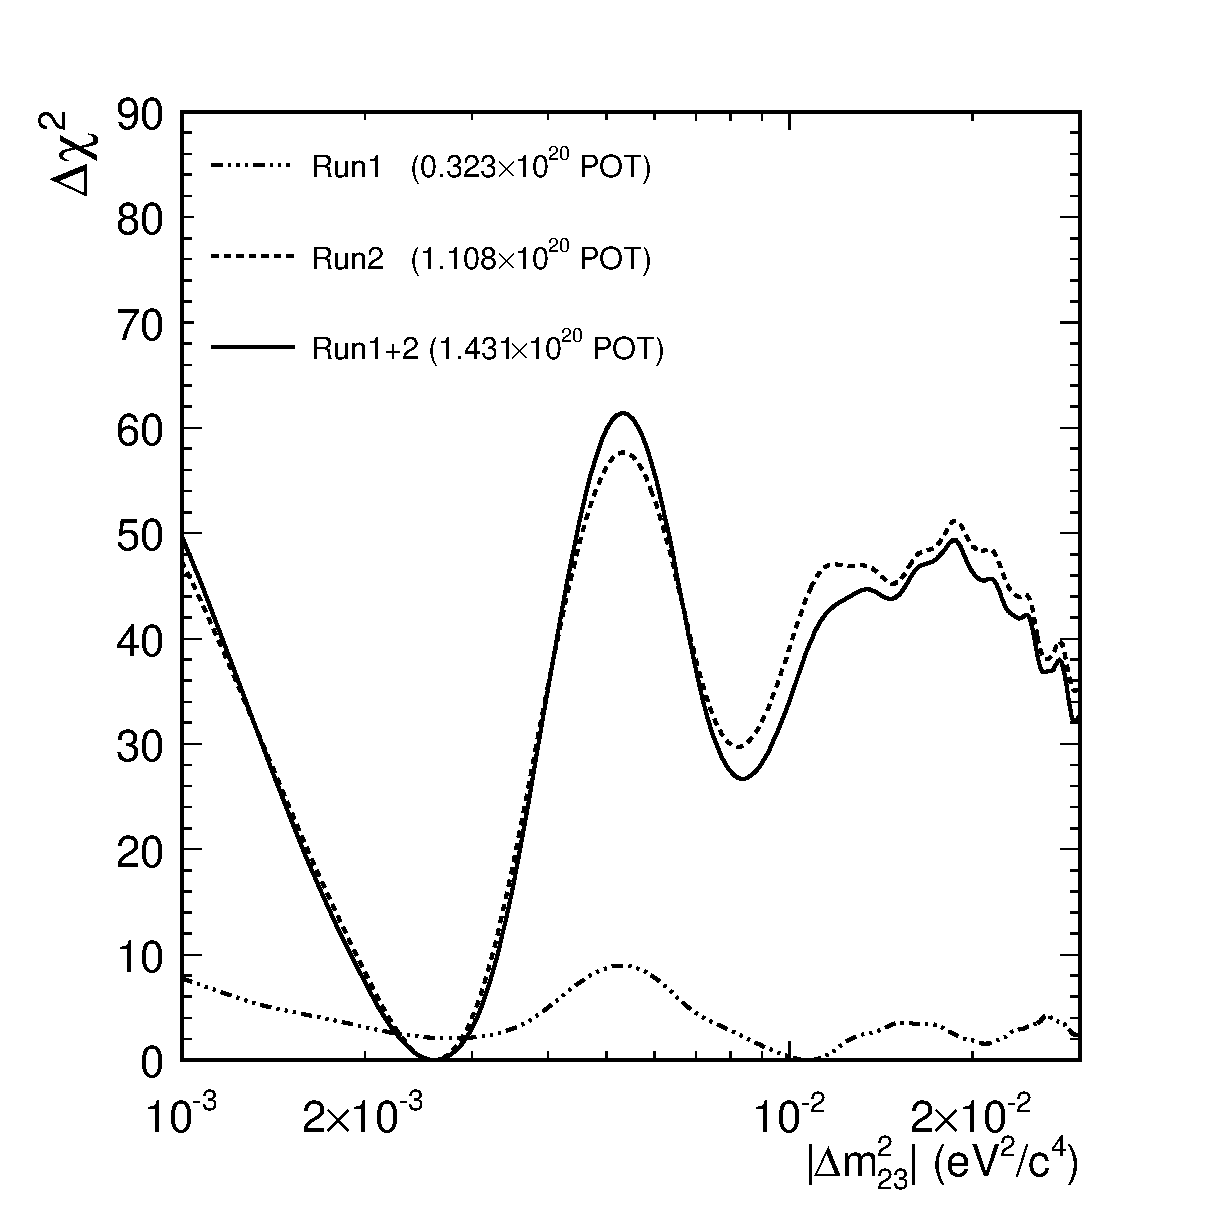
\includegraphics[width=18pc,height=19pc]{./images/fits/neut_marginal_deltachisq_dmsq_wide_3datasets.eps}
\caption{
  The marginalised $\Delta\chi^{2}$ distributions as a function of $|\Delta m^{2}_{23}|$ from the 2-flavour
  $\nu_{\mu}$-disappearance fits to the Run1, Run2 and Run1+2 datasets (NEUT).
  All fits were performed in the extended $|\Delta m^{2}_{23}|$ range from 
  1$\times$10$^{-3}$ $eV^{2}/c^{4}$ to 30$\times$10$^{-3}$ $eV^{2}/c^{4}$.
}
\label{fig:neut_deltachisq_dmsq_wide_3datasets}
\end{minipage}
\end{figure}


% sinsq2theta23
\begin{figure}[ht]
\begin{minipage}[t]{0.47\linewidth}
\centering
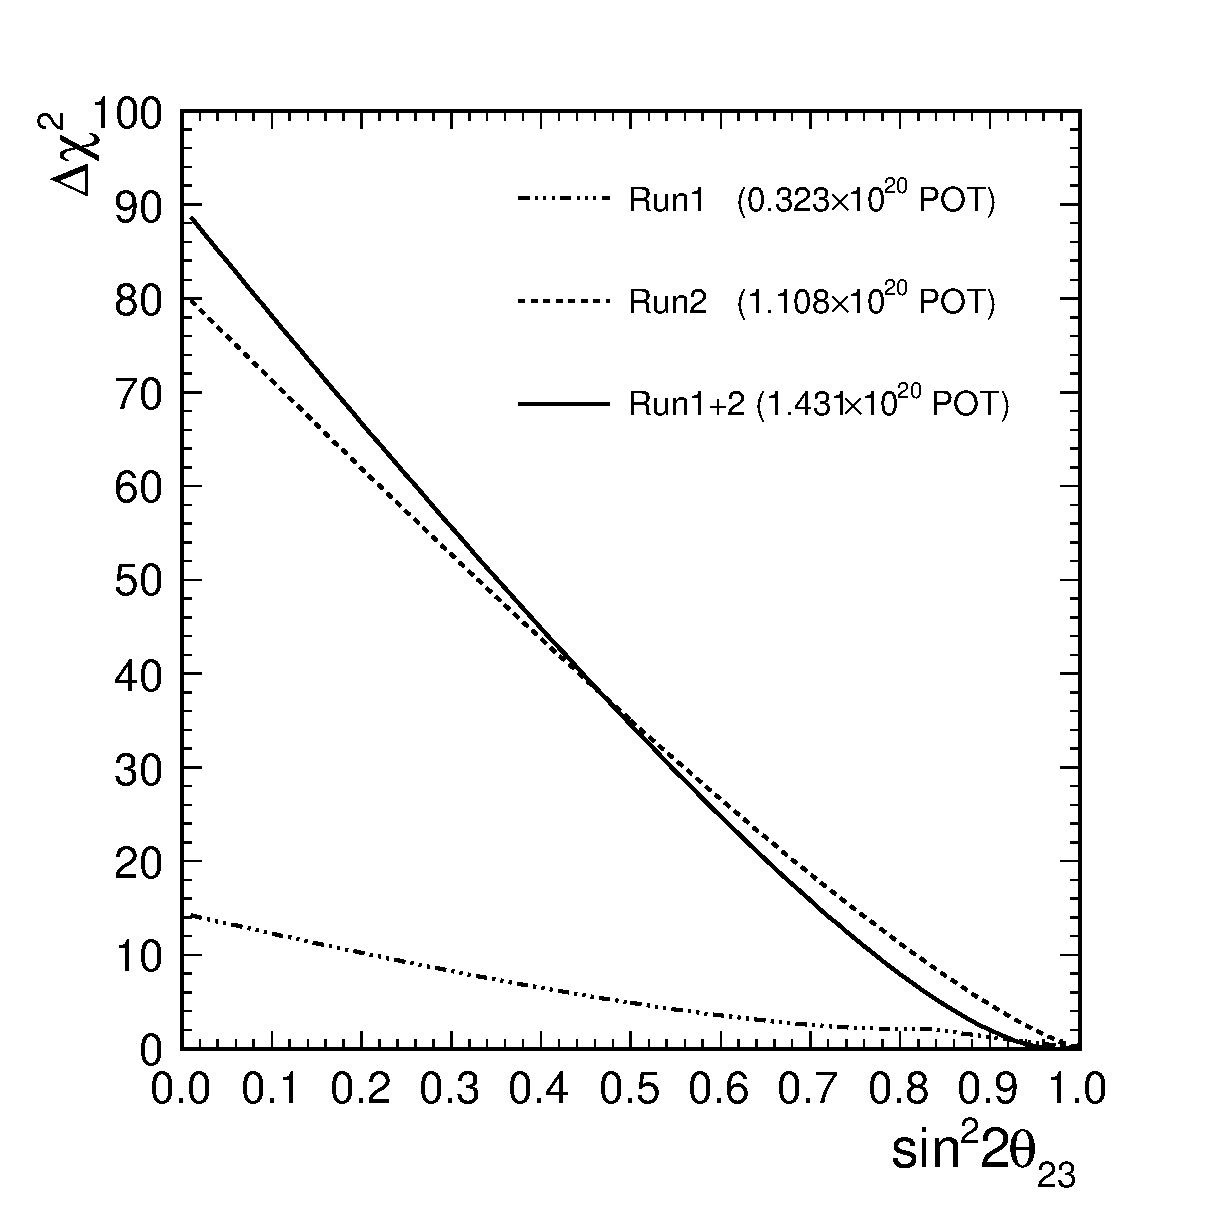
\includegraphics[width=18pc,height=19pc]{./images/fits/genie_marginal_deltachisq_sinsq2theta_3datasets.eps}
\caption{
  The marginalised $\Delta\chi^{2}$ distributions as a function of $sin^{2}2\theta_{23}$ from the 2-flavour
  $\nu_{\mu}$-disappearance fits to the Run1, Run2 and Run1+2 datasets (GENIE).
  All fits were performed in the restricted $|\Delta m^{2}_{23}|$ range from 
  1$\times$10$^{-3}$ $eV^{2}/c^{4}$ to 6$\times$10$^{-3}$ $eV^{2}/c^{4}$.
}
\label{fig:genie_deltachisq_sinsq2theta_3datasets}
\end{minipage}
\hspace{0.06\linewidth}
\begin{minipage}[t]{0.47\linewidth}
\centering  
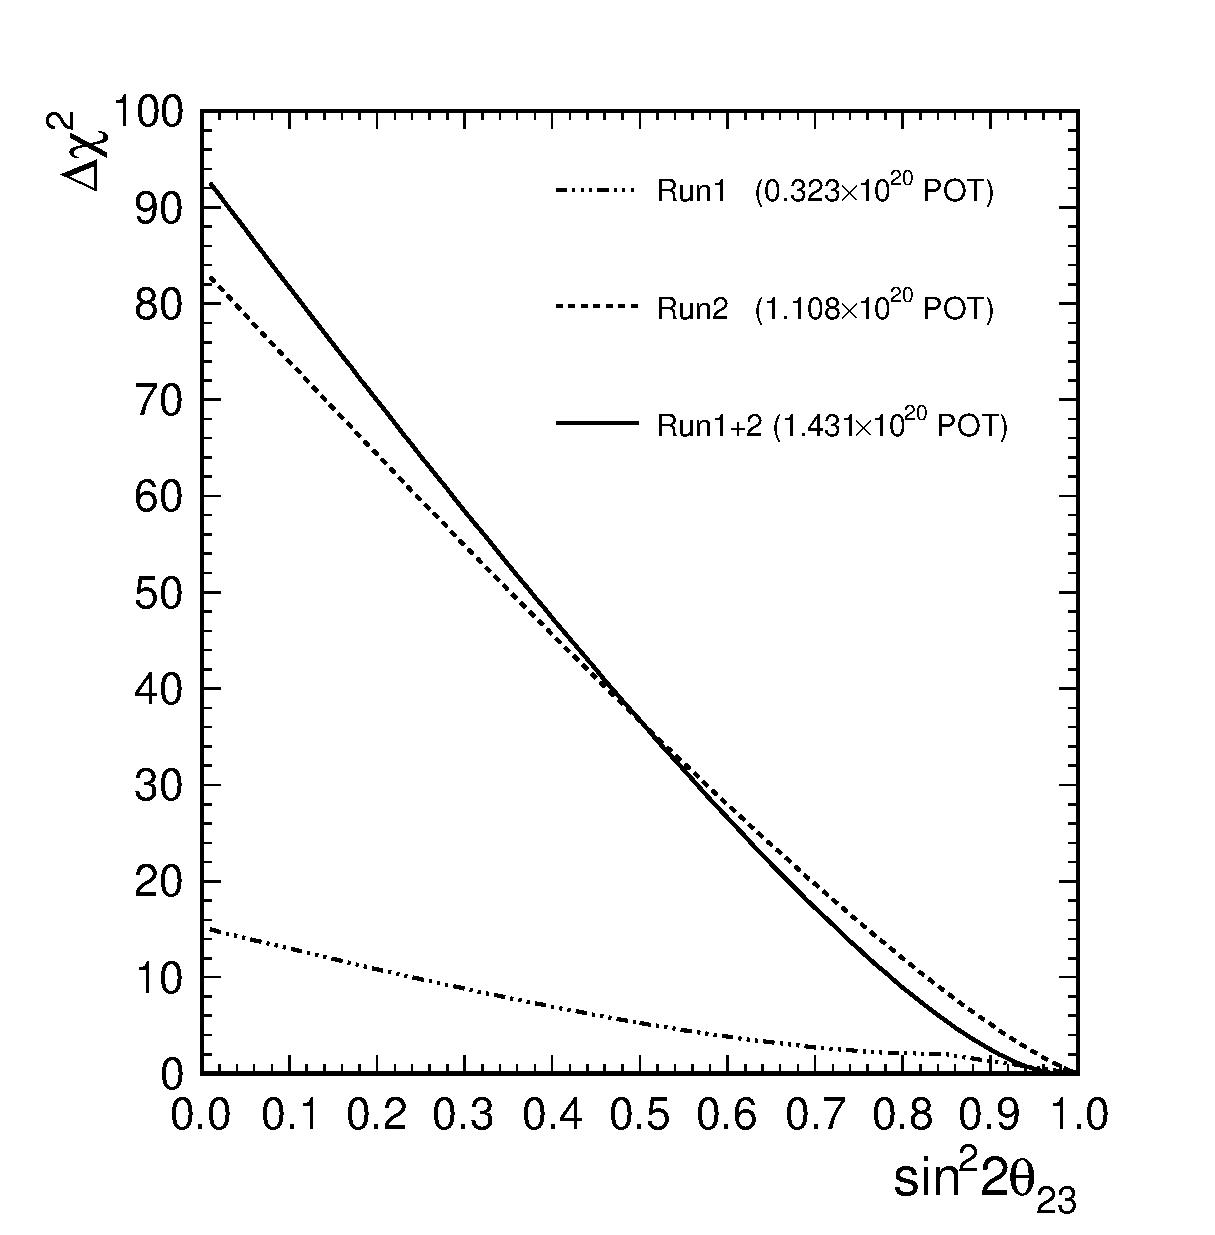
\includegraphics[width=18pc,height=19pc]{./images/fits/neut_marginal_deltachisq_sinsq2theta_3datasets.eps}
\caption{
  The marginalised $\Delta\chi^{2}$ distributions as a function of $sin^{2}2\theta_{23}$ from the 2-flavour
  $\nu_{\mu}$-disappearance fits to the Run1, Run2 and Run1+2 datasets (NEUT).
  All fits were performed in the restricted $|\Delta m^{2}_{23}|$ range from 
  1$\times$10$^{-3}$ $eV^{2}/c^{4}$ to 6$\times$10$^{-3}$ $eV^{2}/c^{4}$.
}
\label{fig:neut_deltachisq_sinsq2theta_3datasets}
\end{minipage}
\end{figure}




\begin{figure*}[htb]
\center
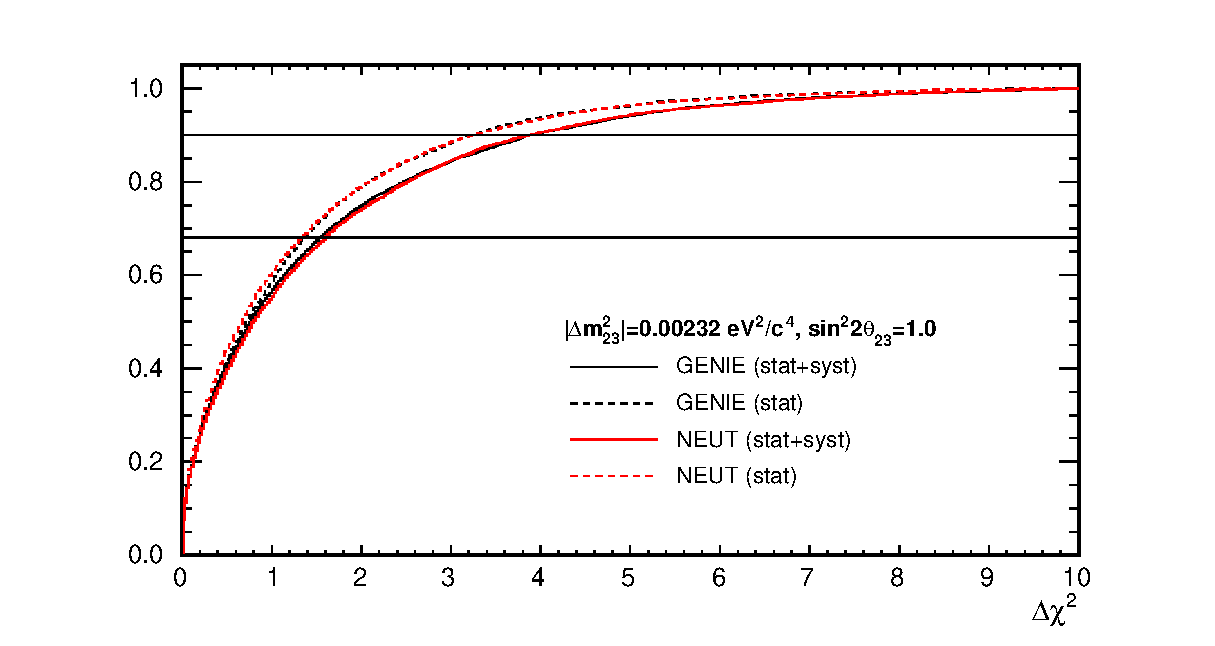
\includegraphics[width=30pc]{./images/feldman_cousins/minos2011_dchisq_cummulative.eps}
\caption{
  Cumulative $\Delta\chi^{2}_{MC}$ distributions (for both NEUT and GENIE) for oscillated toy MC experiments generated
  with $sin^{2}2\theta_{23}$ = 1.0 and $|\Delta m^{2}_{23}|$ = 2.32$\times10^{-3}$ $eV^{2}/c^{4}$.
  The horizontal lines show the 68\% and 90\% levels
  (values of $\Delta\chi^{2}_{critical}$ are the values of $\Delta\chi^{2}_{MC}$ where these horizontal lines
  intersect with the cumulative distributions).
}
\label{fig:minos2011_dchisq_cumulative}
\end{figure*}


\clearpage 

\section {Construction of Feldman-Cousins confidence regions}
\label{sec:fc}

The best-fit $|\Delta m^{2}_{23}|$ fluctuation seen in the analysis of the Run1 dataset is no longer present
(see Figs.\ \ref{fig:genie_deltachisq_dmsq_wide_3datasets} and \ref{fig:neut_deltachisq_dmsq_wide_3datasets}).
The analysis of the Run2 and the combined Run1+2 datasets strongly disfavours any interpretation of the 
observed 1 $\mu$-like ring event deficit in terms of large $|\Delta m^{2}_{23}|$ (a second or higher-order oscillation maximum 
at $\sim$600 MeV). Therefore, for reasons of {\em computational efficiency}, we limit the Feldman-Cousins
construction to the $|\Delta m^{2}_{23}|$ range from 1$\times$10$^{-3}$ $eV^{2}/c^{4}$ to 6$\times$10$^{-3}$ $eV^{2}/c^{4}$.

The application of the Feldman-Cousins method \cite{FeldmanCousins} to the T2K $\nu_{\mu}$-disappearance analysis
is discussed in detail in Sec. 3.4 of Ref. \cite{OurRun1DisappAnalysis}:
a number of toy MC experiment fits is performed for each point of the (sin$^{2}$2$\theta_{23}$, $|\Delta$m$^{2}_{23}|$)
2-dimensional grid.
For each grid point, the critical value of $\Delta\chi^{2}$ ($\Delta\chi^{2}_{critical}$)
is found such that $\alpha$ of the toy MC experiments have $\Delta\chi^{2}_{MC}$ $<$ $\Delta\chi^{2}_{critical}$,
where $\alpha$ is the desired confidence level (see Fig. \ref{fig:minos2011_dchisq_cumulative}).
The value of $\Delta\chi^{2}_{MC}$ for each toy MC experiment is calculated as follows:
\begin{equation}
\displaystyle
\Delta \chi^{2}_{MC} = \chi^{2} \textrm{(true)} - \chi^{2} \textrm{(MC, best-fit)}
\label{eq:deltachi2}
\end{equation}
where
``true'' means the true values of the oscillation parameters at that grid point, and
``best-fit'' means the best-fit values for that MC experiment (this is equivalent to 
equation 5.6 in \cite{FeldmanCousins}).
$\chi^{2}$ is defined as
\begin{equation}
\displaystyle
\chi^{2} (sin^{2}2\theta_{23},|\Delta m^{2}_{23}|;{\bf a}) =
  2 \cdot \sum_{i=0}^{N-1}
   \Big(
     n^{obs}_{i} \cdot ln(n^{obs}_{i}/n^{exp}_{i}) +
     (n^{exp}_{i}-n^{obs}_{i})
   \Big) 
\label{eq:chisquare}
\end{equation}
where
$N$ is the number of reconstructed energy bins,
${\bf a}$ is a vector of nuisance parameters (see Tab. \ref{tab:input_uncertainties}),
$n^{obs}_{i}$ is the observed number of events in the $i^{th}$ bin, and
$n^{exp}_{i} = n^{exp}_{i}(sin^{2}2\theta_{23},\Delta m^{2}_{23}; {\bf a})$
is the corresponding expected number of events. This definition of $\chi^{2}$ arises from our use
of the likelihood ratio method, which is explained in more detail in 
Sec.\ 3.2 of Ref.\ \cite{OurRun1DisappAnalysis}.

\section {Run 1+2 oscillation parameter confidence regions }
\label{sec:conf_regions}

Feldman-Cousins confidence regions were constructed using the 
$\Delta\chi^{2}$(sin$^{2}$2$\theta_{23}$, $|\Delta$m$^{2}_{23}|$) surfaces
from the fits presented in Sec.\ \ref{sec:fits} and the
$\Delta\chi^{2}_{critical}$(sin$^{2}$2$\theta_{23}$, $|\Delta$m$^{2}_{23}|$) maps
presented in Sec.\ \ref{sec:fc}.

The 68\% and 90\% Feldman-Cousins confidence regions are shown for the
2-flavour $\nu_{\mu}$-disappearance fit to the combined Run1+2 dataset 
with and without systematics
in Fig.\ \ref{fig:contour_run1p2_statsyst_genie} for GENIE and
in Fig.\ \ref{fig:contour_run1p2_statsyst_neut} for NEUT.
(It is worth noting that all confidence regions presented here are drawn
using a $sin^{2}2\theta_{23}$ bin size of 0.01 and 
a $|\Delta m^{2}_{23}|$ bin size of 1.0$\times10^{-4}$ $eV^{2}/c^{4}$).
The star-shaped marker in each plot marks the bin with the minimum $\chi^{2}$.)
The 90\% confidence regions are compared with those from 
MINOS \cite{Minos2011} and SuperK \cite{OldDisappSuperK}
in Fig.\ \ref{fig:contour_run1p2_statsyst_genie_external_90cl} for GENIE and
in Fig.\ \ref{fig:contour_run1p2_statsyst_neut_external_90cl} for NEUT.
A similar comparison is shown in Figs.
\ref{fig:contour_run1p2_statsyst_genie_external} and
\ref{fig:contour_run1p2_statsyst_neut_external}, and
includes the 68\% confidence regions from T2K and MINOS.

In Fig.\ \ref{fig:contour_run1p2_statsyst_genie_minos11sens}
the 90\% Feldman-Cousins confidence region (with systematics) from the GENIE
2-flavour $\nu_{\mu}$-disappearance fit to the combined Run1+2 dataset 
is compared with the T2K $1.431 \times 10^{20}$ POT sensitivity for oscillations
with the 2011 MINOS best-fit values
($sin^{2}2\theta_{23}$ = 1.0 and $|\Delta m^{2}_{23}|$ = 2.32$\times10^{-3}$ $eV^{2}/c^{4}$).
The 2011 MINOS 90\% confidence region is also shown in this figure.
The equivalent comparison from the NEUT 2-flavour $\nu_{\mu}$-disappearance fit is shown in 
Fig.\ \ref{fig:contour_run1p2_statsyst_neut_minos11sens}.

The 90\% Feldman-Cousins confidence region from the fit to the combined Run1+2 dataset
is compared with the 90\% confidence regions from the fits to the Run1-only and Run2-only datasets 
in Fig.\ \ref{fig:contour_statsyst_genie_3datasets} for GENIE and
in Fig.\ \ref{fig:contour_statsyst_neut_3datasets} for NEUT.

Finally, a comparison of the GENIE and NEUT 90\% Feldman-Cousins confidence regions 
from the fit to the combined Run1+2 dataset 
is shown in Fig.\ \ref{fig:contour_statsyst_genie_neut_comparison}.


%
% --------------------------------------------------------------------------------------------------------------------
%

% plot moved to previous section (numuosc2_contours.tex) to avoid having 2 half-empty pages
%
%\begin{figure*}[htb]
%\center
%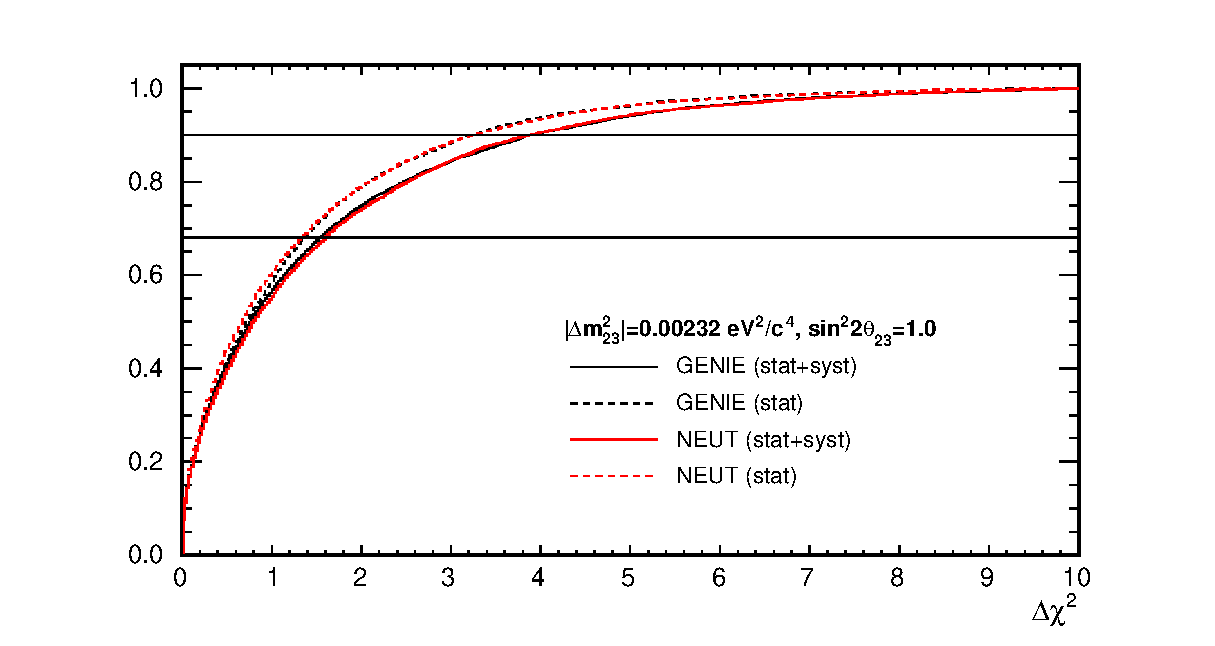
\includegraphics[width=24pc]{./images/feldman_cousins/minos2011_dchisq_cummulative.eps}
%\caption{
%  Cumulative $\Delta\chi^{2}_{MC}$ distributions (for both NEUT and GENIE) for oscillated toy MC experiments generated
%  with $sin^{2}2\theta_{23}$ = 1.0 and $|\Delta m^{2}_{23}|$ = 2.32$\times10^{-3}$ $eV^{2}/c^{4}$.
%  The horizontal lines show the 68\% and 90\% levels
%  (values of $\Delta\chi^{2}_{critical}$ are the values of $\Delta\chi^{2}_{MC}$ where these horizontal lines
%  intersect with the cumulative distributions).
%}
%\label{fig:minos2011_dchisq_cumulative}
%\end{figure*}

\begin{figure*}[htb]
\center
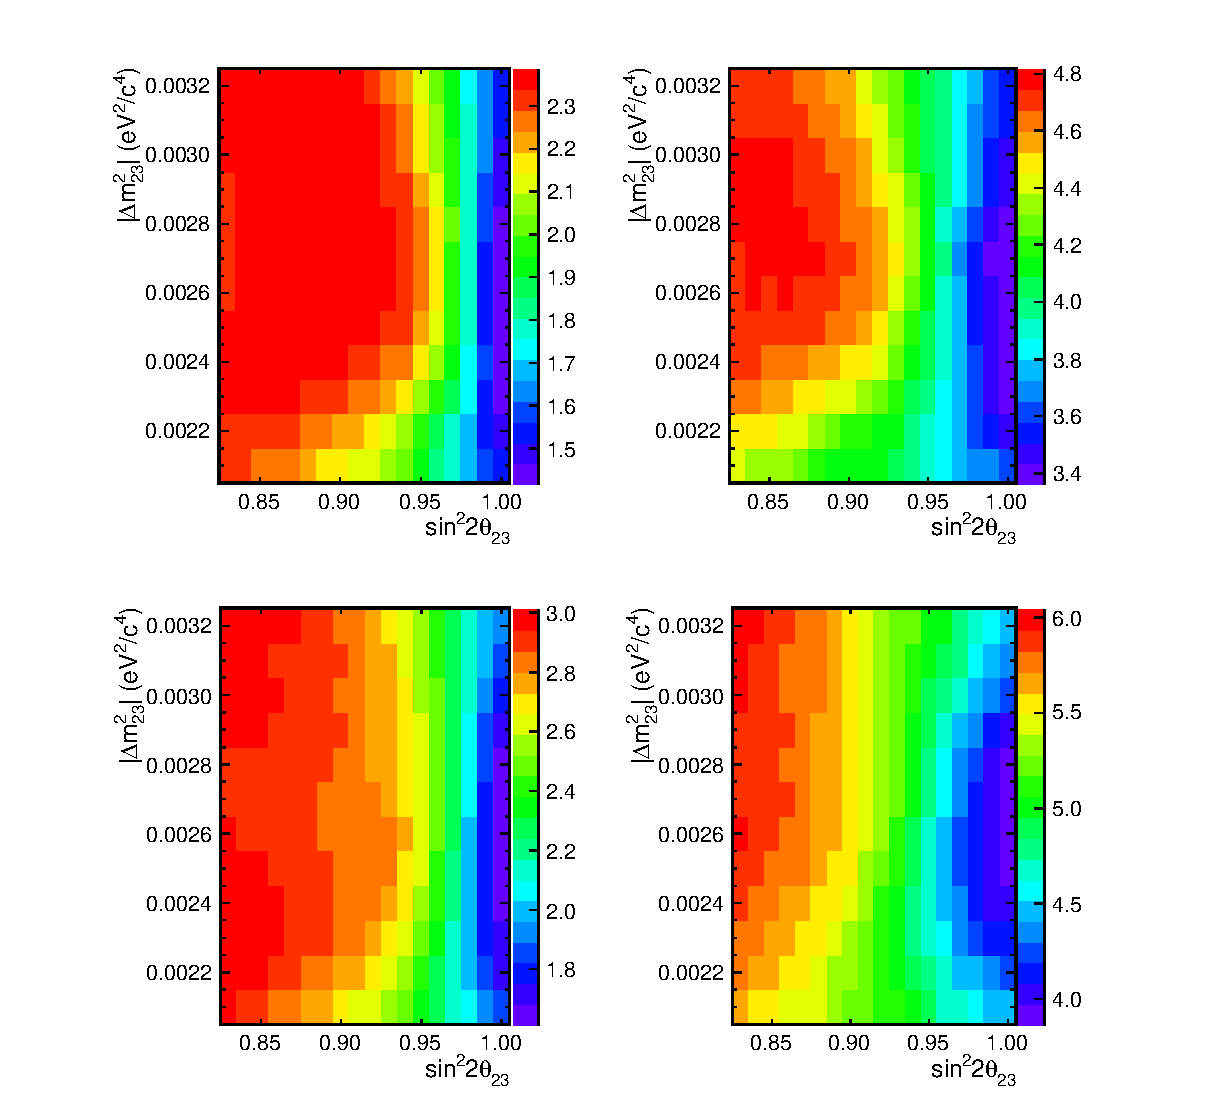
\includegraphics[width=42pc]{./images/feldman_cousins/fc_deltachisqcrit_2d_neut.eps}
\caption{
  Monte Carlo estimation,
  according to the Feldman-Cousins method,
  of $\Delta\chi^{2}_{68}$ (left) and $\Delta\chi^{2}_{90}$ (right)
  as functions of $sin^{2}{2\theta_{23}}$ and $\Delta{m^{2}_{23}}$,
  for calculation of the 68\% (left) and 90\% (right) CL confidence regions
  for the $1.431 \times 10^{20}$-POT T2K 2-flavour $\nu_{\mu}$-disappearance analysis.
  The top row shows $\Delta\chi^{2}$ surfaces calculated using statistical fluctuations
  only whereas the bottom row shows $\Delta\chi^{2}$ surfaces calculated using
  both systematic variations and statistical fluctations.
  As expected from \cite{FeldmanCousins}, the values of $\Delta\chi^{2}$ 
  decrease as the
  physical boundary at $sin^{2}{2\theta_{23}}$ = 1 is approached. 
}
\label{fig:fc_deltachisqcrit_2d_neut}
\end{figure*}


\begin{figure*}[htb]
\center
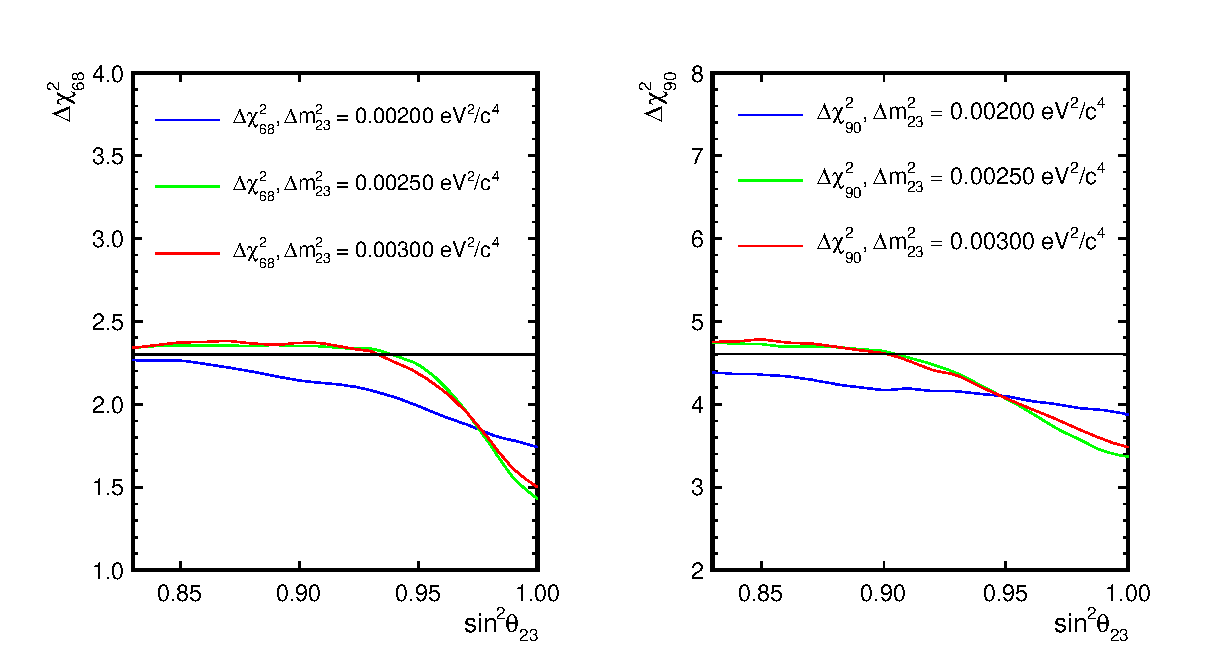
\includegraphics[width=38pc]{./images/feldman_cousins/fc_deltachisqcrit_statonly_vs_sinsq_3dmsq_neut.eps}
\caption{
  Monte Carlo estimation,
  according to the Feldman-Cousins method (statistical errors only),
  of $\Delta\chi^{2}_{68}$ (left) and $\Delta\chi^{2}_{90}$ (right),
  as functions of $sin^{2}{2\theta_{23}}$ for 3 different values of $\Delta{m^{2}_{23}}$
  ($2.0 \times 10^{-3} eV^{2}/c^{4}$,
   $2.5 \times 10^{-3} eV^{2}/c^{4}$ and
   $3.0 \times 10^{-3} eV^{2}/c^{4}$).
  For comparison, the canonical value of $\Delta\chi^{2}$ used in the constant $\Delta\chi^{2}_{critical}$
  method is also shown as a horizontal line.
}
\label{fig:fc_deltachisqcrit_statonly_vs_sinsq_3dmsq_neut}
\end{figure*}

\begin{figure*}[htb]
\center
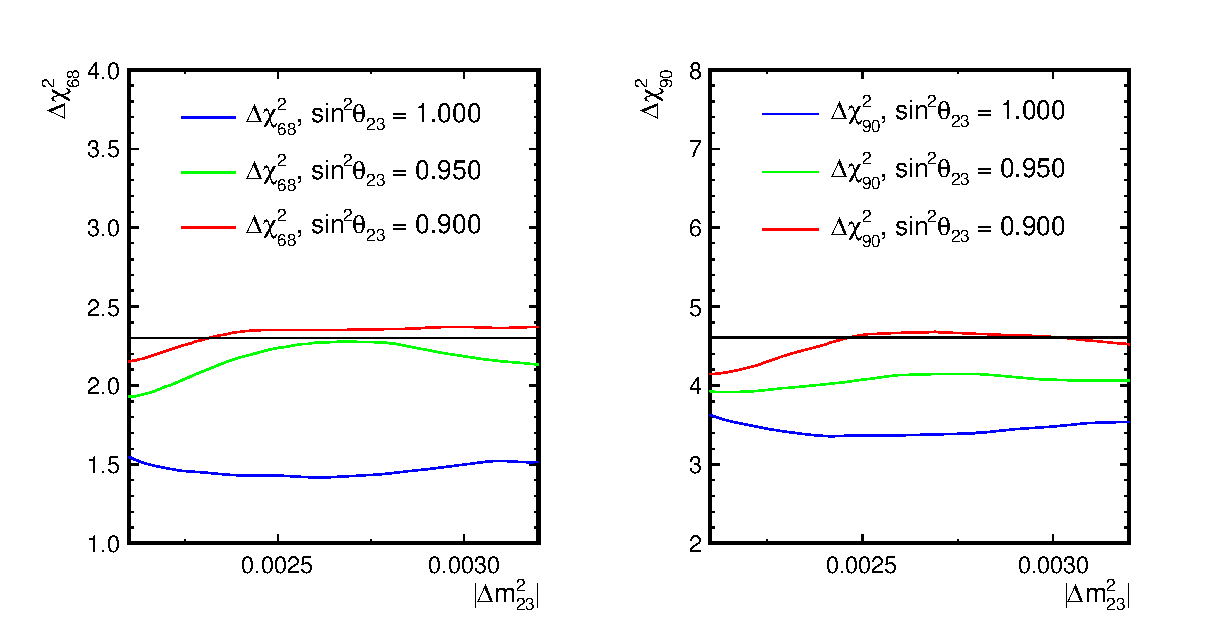
\includegraphics[width=38pc]{./images/feldman_cousins/fc_deltachisqcrit_statonly_vs_dmsq_3sinsq_neut.eps}
\caption{
  Monte Carlo estimation,
  according to the Feldman-Cousins method (statistical errors only),
  of $\Delta\chi^{2}_{68}$ (left) and $\Delta\chi^{2}_{90}$ (right),
  as functions of $\Delta{m^{2}_{23}}$ for 3 different values of $sin^{2}{2\theta_{23}}$
  (0.90, 0.95 and 1.00).
  For comparison, the canonical value of $\Delta\chi^{2}$ used in the constant $\Delta\chi^{2}_{critical}$
  method is also shown as a horizontal line.
}
\label{fig:fc_deltachisqcrit_statonly_vs_dmsq_3sinsq_neut}
\end{figure*}



%
% confidence regions for the Run1+2 fit
%

\begin{figure*}[htb]
\center
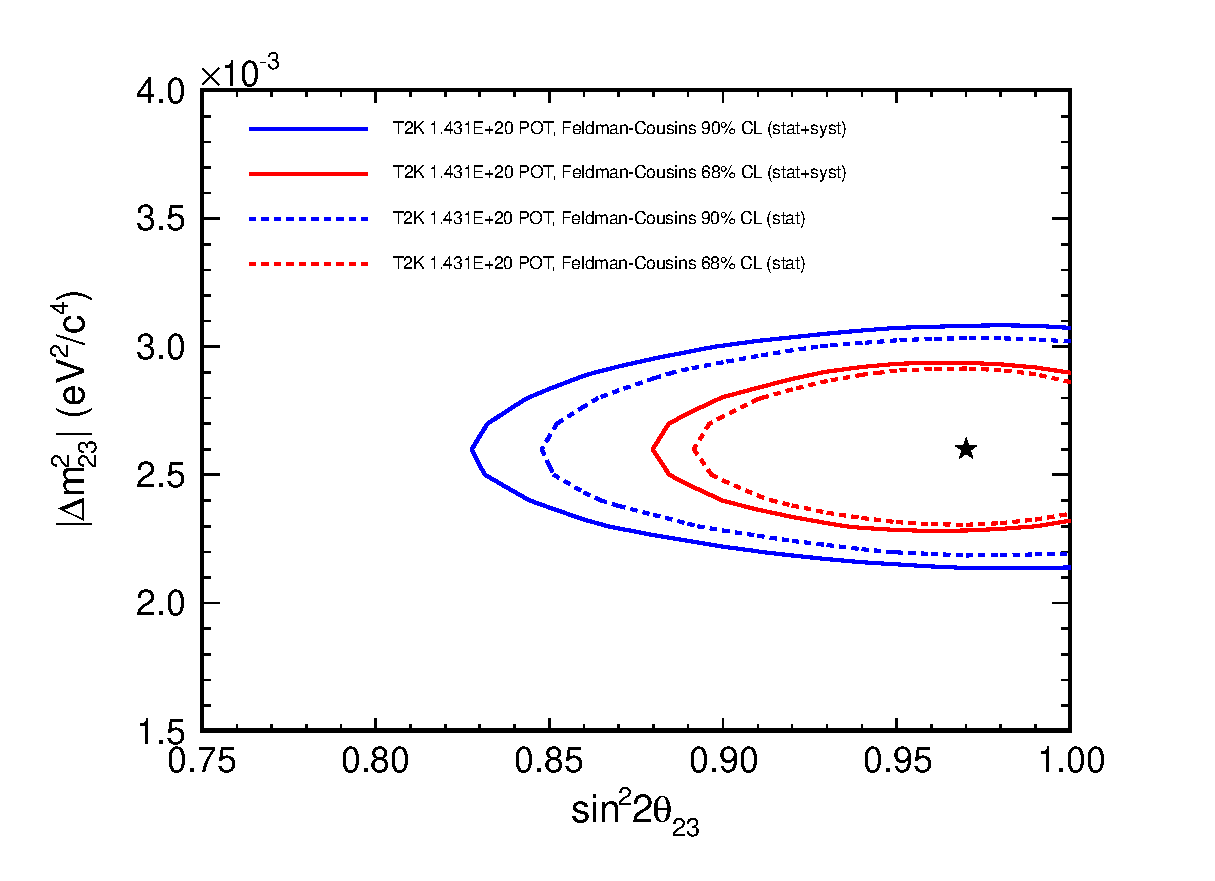
\includegraphics[width=30pc]{./images/confidence_regions/contour_run1p2_statsyst_genie.eps}
\caption{
  68\% and 90\% Feldman-Cousins confidence regions, with and without systematics,
  for the GENIE 2-flavour $\nu_{\mu}$-disappearance fit to the combined Run1+2 dataset
}
\label{fig:contour_run1p2_statsyst_genie}
\end{figure*}


\begin{figure*}[htb]
\center
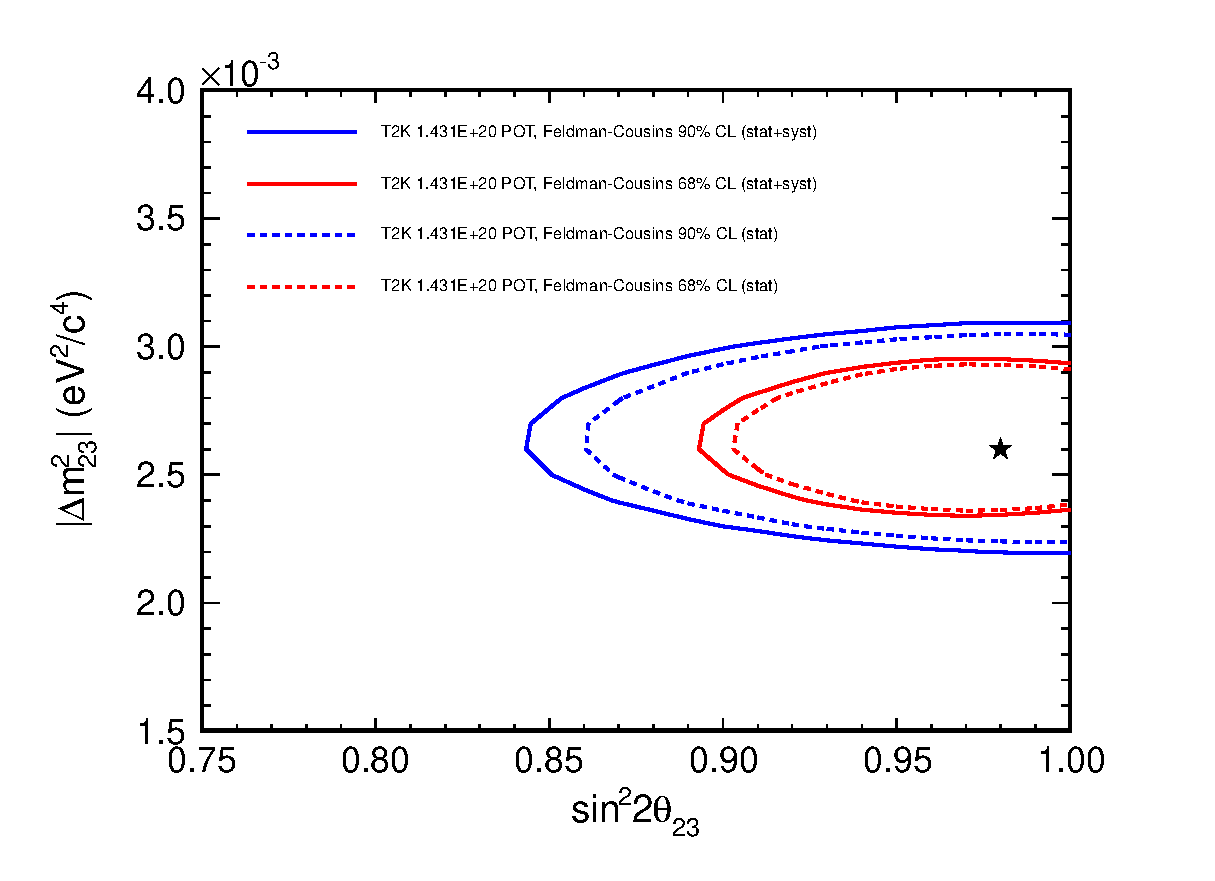
\includegraphics[width=30pc]{./images/confidence_regions/contour_run1p2_statsyst_neut.eps}
\caption{
  68\% and 90\% Feldman-Cousins confidence regions, with and without systematics,
  for the NEUT 2-flavour $\nu_{\mu}$-disappearance fit to the combined Run1+2 dataset
}
\label{fig:contour_run1p2_statsyst_neut}
\end{figure*}

%
% confidence regions for the Run1+2 fit - comparison with MINOS/K2K/SK-atm
%

\begin{figure*}[htb]
\center
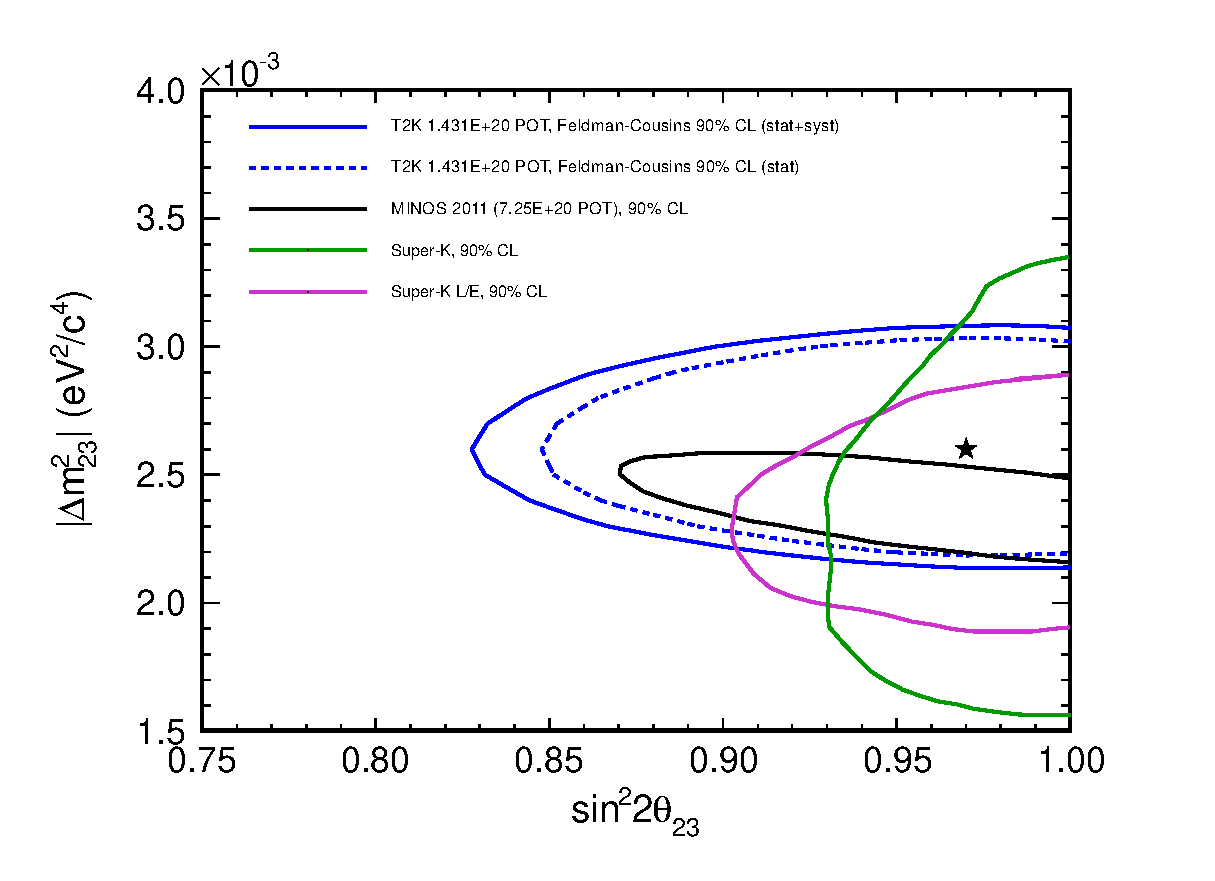
\includegraphics[width=30pc]{./images/confidence_regions/contour_run1p2_statsyst_genie_external_90clonly.eps}
\caption{
  90\% Feldman-Cousins confidence regions, with and without systematics,
  for the GENIE 2-flavour $\nu_{\mu}$-disappearance fit to the combined Run1+2 dataset:
  comparisons with results from MINOS \cite{Minos2011} and SuperK \cite{OldDisappSuperK}.
}
\label{fig:contour_run1p2_statsyst_genie_external_90cl}
\end{figure*}

\begin{figure*}[htb]
\center
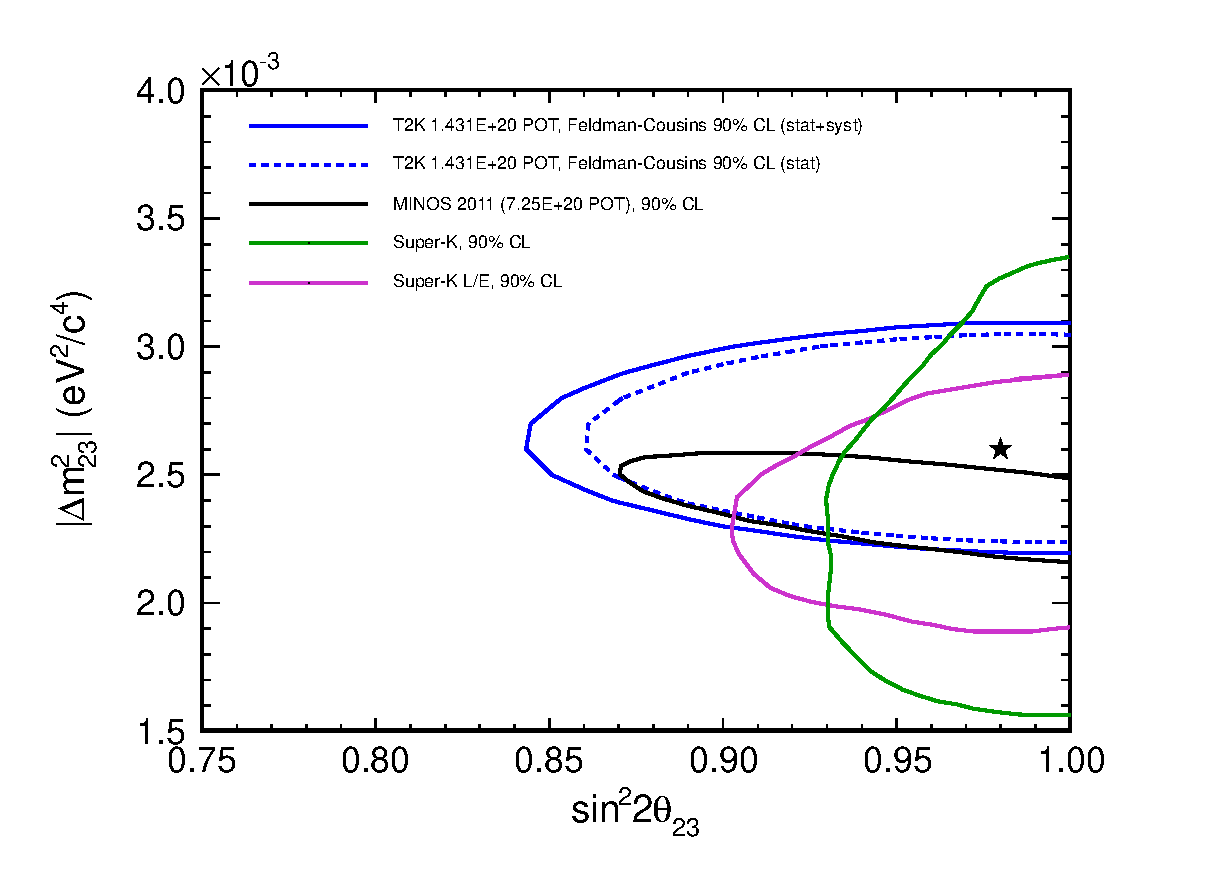
\includegraphics[width=30pc]{./images/confidence_regions/contour_run1p2_statsyst_neut_external_90clonly.eps}
\caption{
  90\% Feldman-Cousins confidence regions, with and without systematics,
  for the NEUT 2-flavour $\nu_{\mu}$-disappearance fit to the combined Run1+2 dataset:
  comparisons with results from MINOS \cite{Minos2011} and SuperK \cite{OldDisappSuperK}.
}
\label{fig:contour_run1p2_statsyst_neut_external_90cl}
\end{figure*}


%
% confidence regions for the Run1+2 fit - comparison with MINOS/K2K/SK-atm
%

\begin{figure*}[htb]
\center
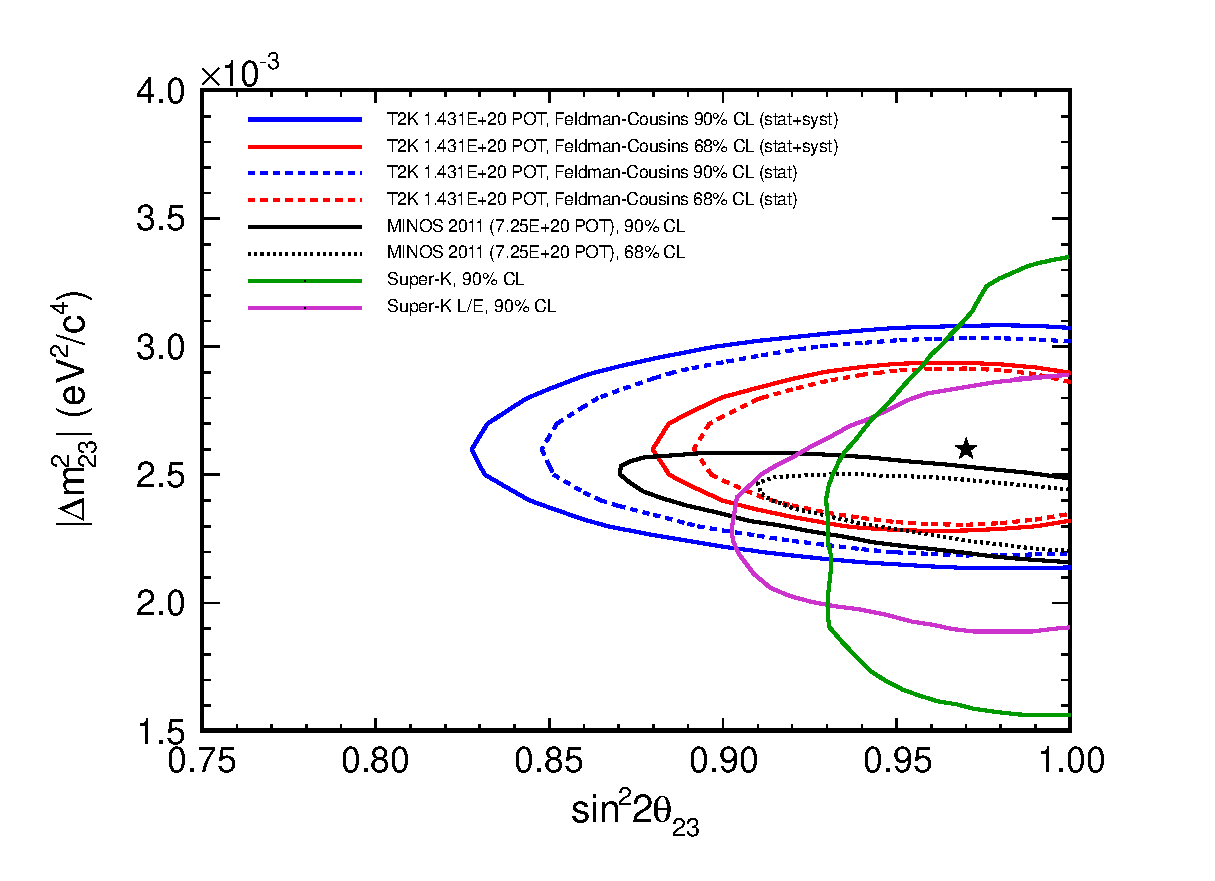
\includegraphics[width=30pc]{./images/confidence_regions/contour_run1p2_statsyst_genie_external.eps}
\caption{
  68\% and 90\% Feldman-Cousins confidence regions, with and without systematics,
  for the GENIE 2-flavour $\nu_{\mu}$-disappearance fit to the combined Run1+2 dataset:
  comparisons with MINOS 2011 68\% and 90\% contours \cite{Minos2011} and SuperK 90\% contour \cite{OldDisappSuperK}.
}
\label{fig:contour_run1p2_statsyst_genie_external}
\end{figure*}

\begin{figure*}[htb]
\center
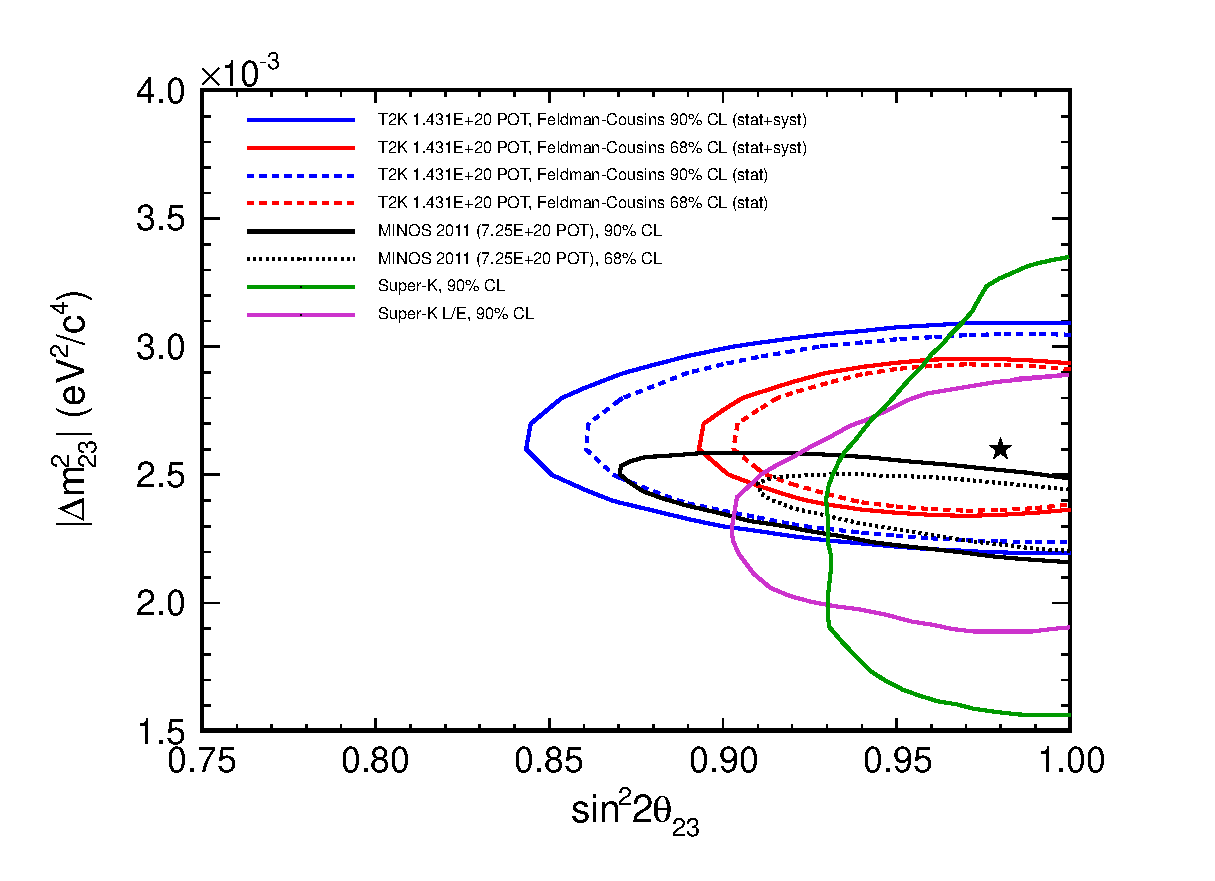
\includegraphics[width=30pc]{./images/confidence_regions/contour_run1p2_statsyst_neut_external.eps}
\caption{
  68\% and 90\% Feldman-Cousins confidence regions, with and without systematics,
  for the NEUT 2-flavour $\nu_{\mu}$-disappearance fit to the combined Run1+2 dataset:
  comparisons with MINOS 2011 68\% and 90\% contours \cite{Minos2011} and SuperK 90\% contour \cite{OldDisappSuperK}.
}
\label{fig:contour_run1p2_statsyst_neut_external}
\end{figure*}


%
% confidence regions for the Run1+2 fit - comparison with sensitivity for MINOS-2011 params
%

\begin{figure*}[htb]
\center
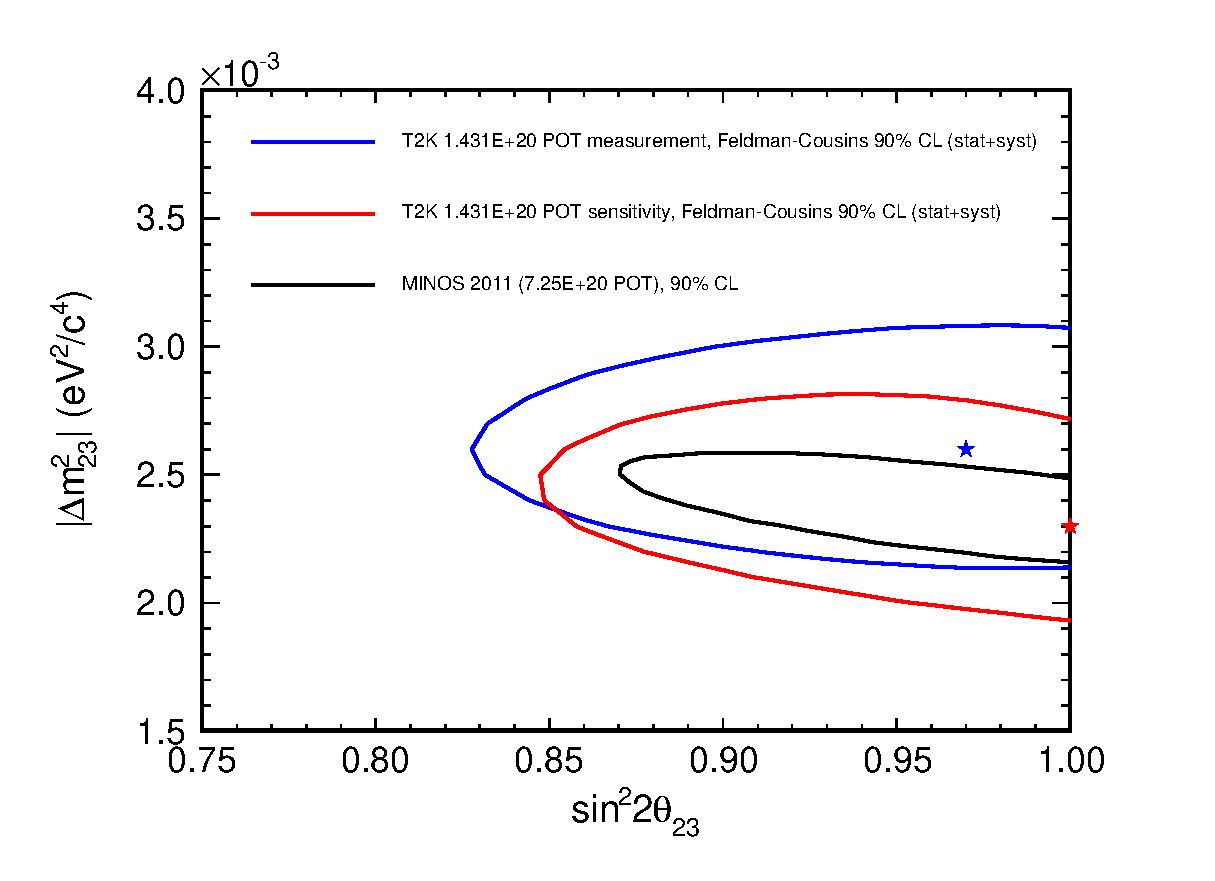
\includegraphics[width=30pc]{./images/confidence_regions/contour_run1p2_statsyst_genie_minos11sens.eps}
\caption{
  90\% Feldman-Cousins confidence regions (with systematics)
  for the GENIE 2-flavour $\nu_{\mu}$-disappearance fit to the combined Run1+2 dataset:
  comparisons with T2K 1.431$\times$10$^{20}$ POT sensitivity for $\nu_{\mu}$-disappearance with the MINOS 2011 
  best-fit values ($sin^{2}2\theta_{23}$ = 1.0 and $|\Delta m^{2}_{23}|$ = 2.32$\times10^{-3}$ $eV^{2}/c^{4}$).
  The MINOS 2011 90\% confidence region \cite{Minos2011} is also shown.
}
\label{fig:contour_run1p2_statsyst_genie_minos11sens}
\end{figure*}

\begin{figure*}[htb]
\center
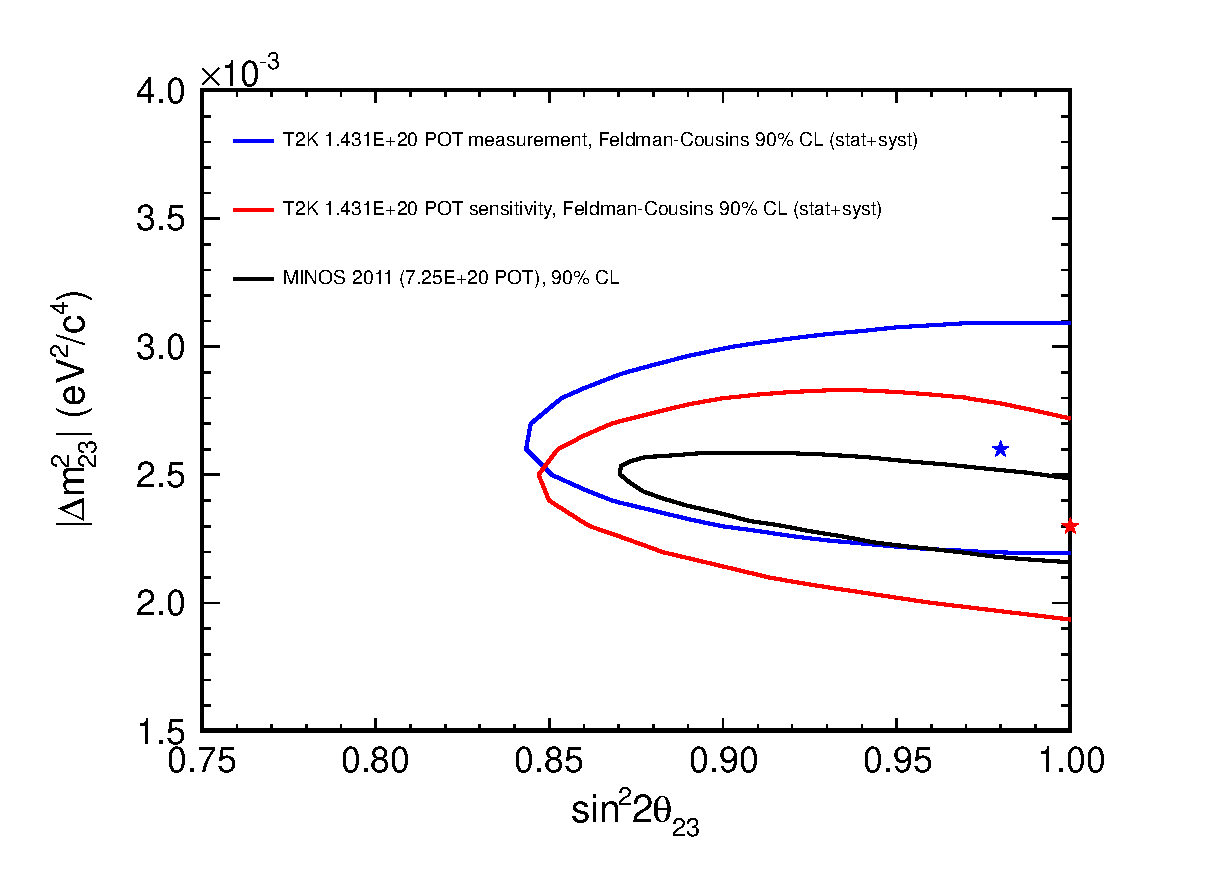
\includegraphics[width=30pc]{./images/confidence_regions/contour_run1p2_statsyst_neut_minos11sens.eps}
\caption{
  90\% Feldman-Cousins confidence regions (with systematics)
  for the NEUT 2-flavour $\nu_{\mu}$-disappearance fit to the combined Run1+2 dataset:
  comparisons with T2K 1.431$\times$10$^{20}$ POT sensitivity for $\nu_{\mu}$-disappearance with the MINOS 2011 
  best-fit values ($sin^{2}2\theta_{23}$ = 1.0 and $|\Delta m^{2}_{23}|$ = 2.32$\times10^{-3}$ $eV^{2}/c^{4}$).
  The MINOS 2011 90\% confidence region \cite{Minos2011} is also shown.
}
\label{fig:contour_run1p2_statsyst_neut_minos11sens}
\end{figure*}



%
% confidence regions for the Run1, Run2 and Run1+2 fits
%

\begin{figure*}[htb]
\center
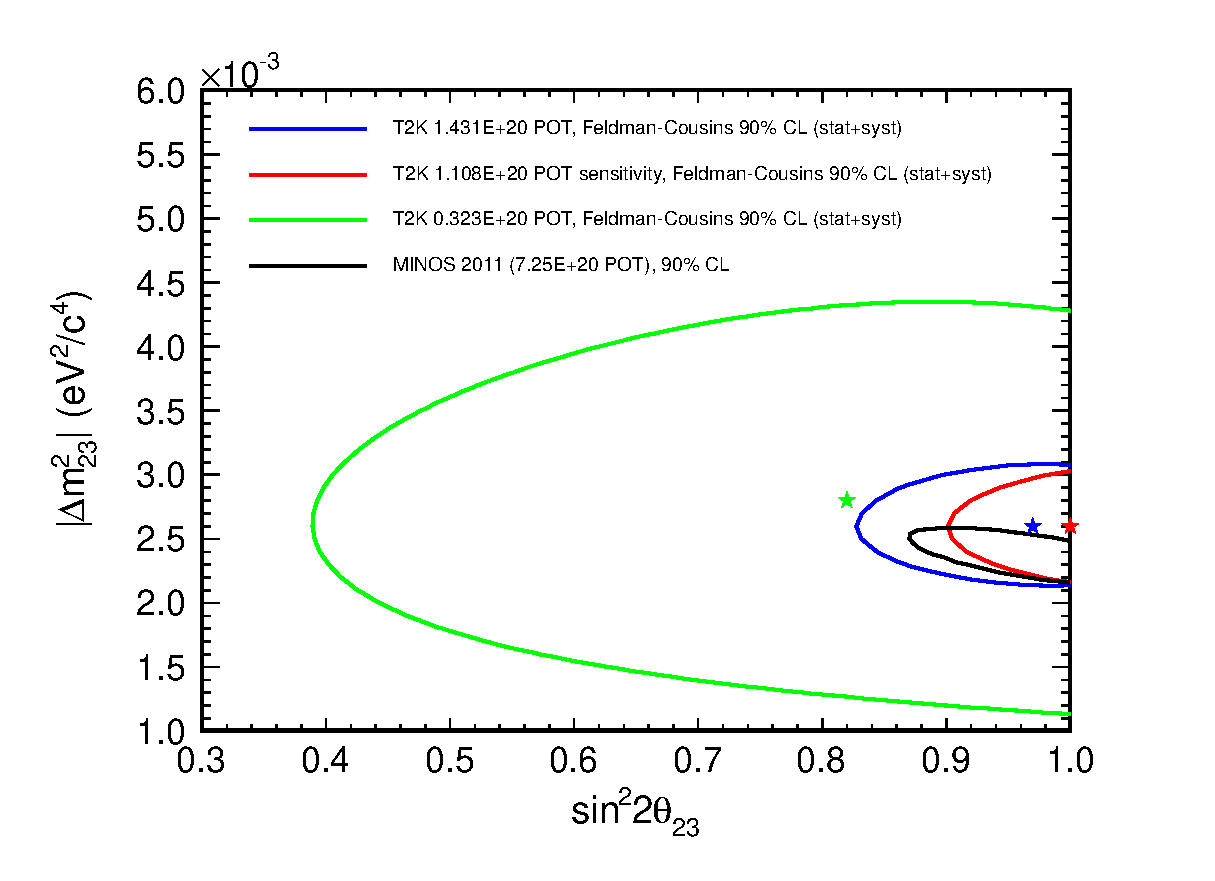
\includegraphics[width=30pc]{./images/confidence_regions/contour_statsyst_genie_3datasets.eps}
\caption{
  90\% Feldman-Cousins confidence regions (with systematics)
  for the GENIE 2-flavour $\nu_{\mu}$-disappearance fits to the Run1, Run2 and the combined Run1+2 datasets.
  The MINOS 2011 result \cite{Minos2011} is also shown for reference.
}
\label{fig:contour_statsyst_genie_3datasets}
\end{figure*}

\begin{figure*}[htb]
\center
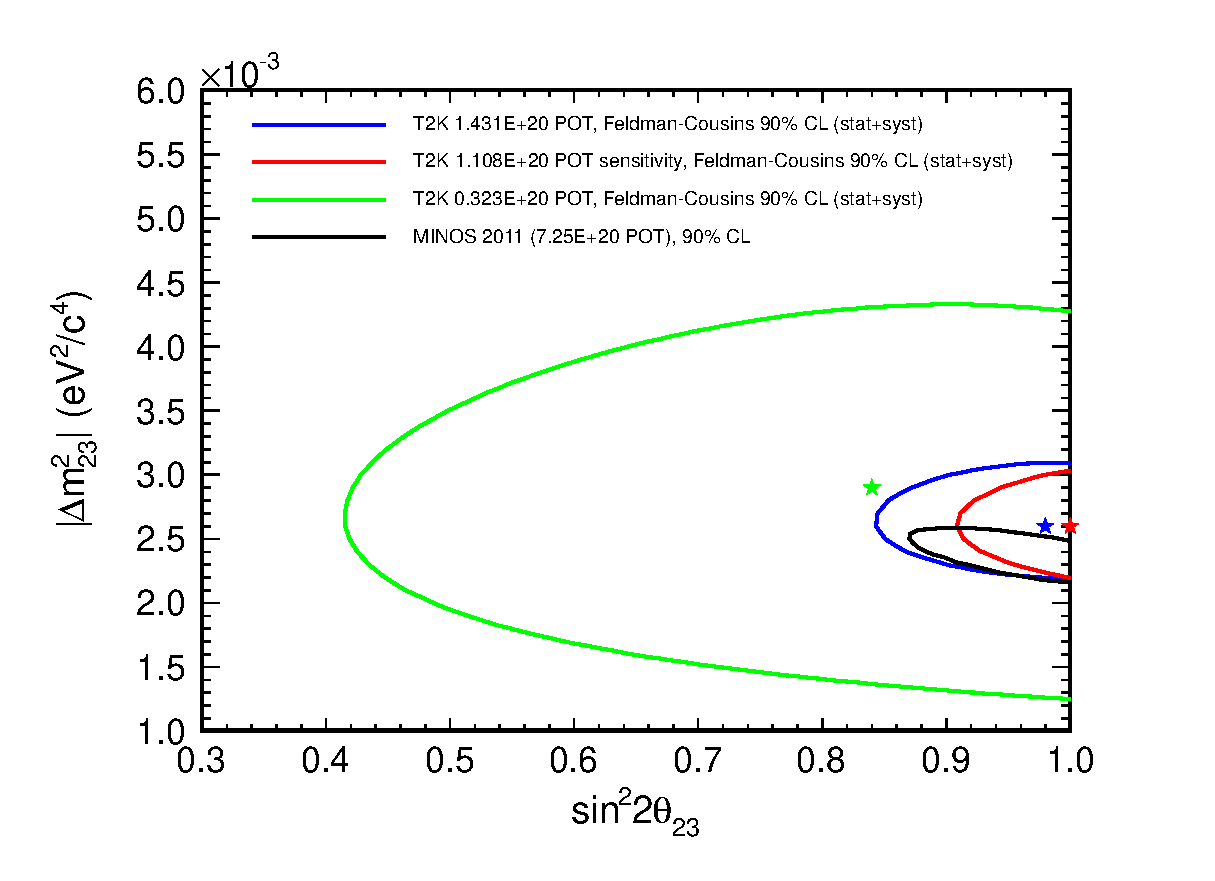
\includegraphics[width=30pc]{./images/confidence_regions/contour_statsyst_neut_3datasets.eps}
\caption{
  90\% Feldman-Cousins confidence regions (with systematics)
  for the NEUT 2-flavour $\nu_{\mu}$-disappearance fits to the Run1, Run2 and the combined Run1+2 datasets.
  The MINOS 2011 result \cite{Minos2011} is also shown for reference.
}
\label{fig:contour_statsyst_neut_3datasets}
\end{figure*}


%
% comparison of GENIE and NEUT Run1+2 contours
%

\begin{figure*}[htb]
\center
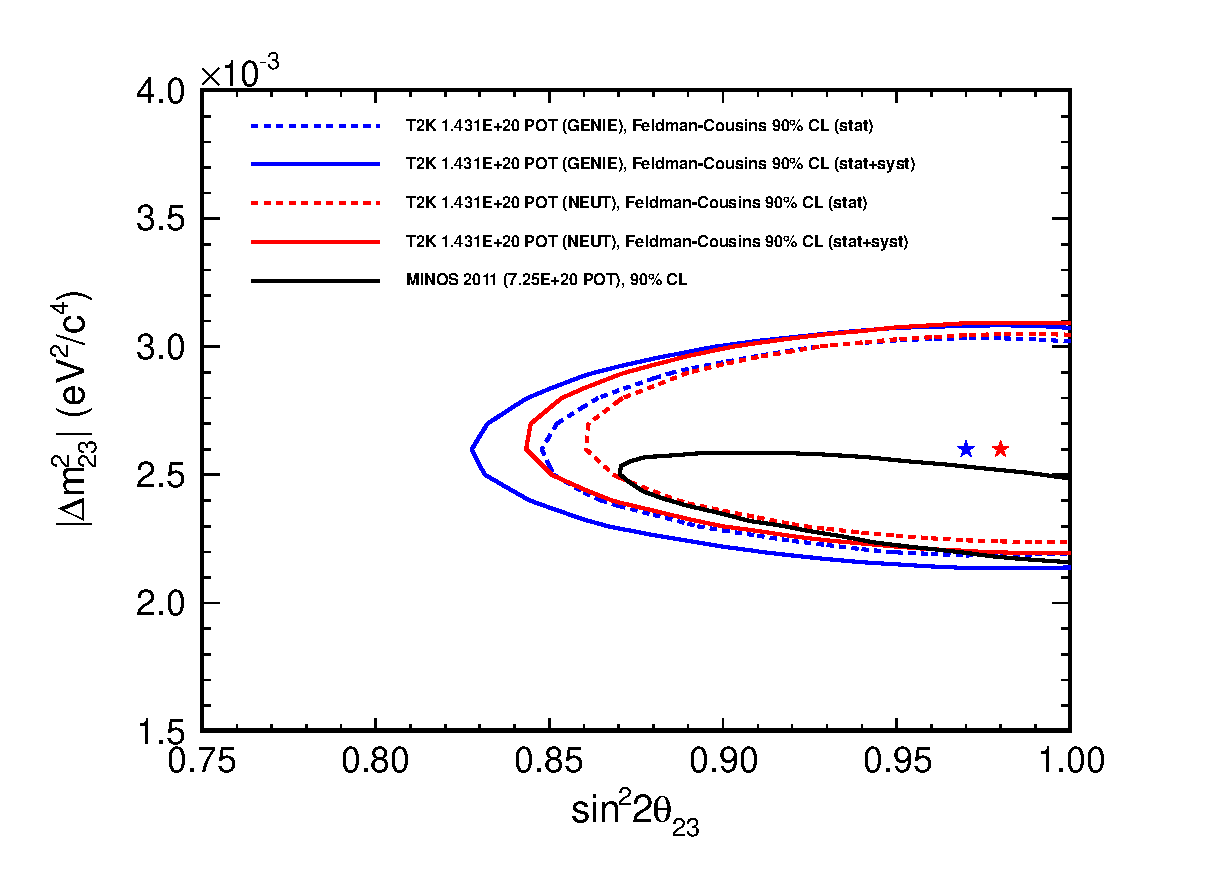
\includegraphics[width=30pc]{./images/confidence_regions/contour_run1p2_genie_neut_comparison.eps}
\caption{
  Comparison of the GENIE and NEUT 90\% Feldman-Cousins confidence regions (with and witout systematics)
  for the 2-flavour $\nu_{\mu}$-disappearance fits to the combined Run1+2 dataset.
  The MINOS 2011 result \cite{Minos2011} is also shown for reference.
}
\label{fig:contour_statsyst_genie_neut_comparison}
\end{figure*}


\clearpage 

\section {Summary }
\label{sec:summary}

In this note, we have presented the results of a 2-flavour $\nu_{\mu}$-disappearance analysis 
on the combined Run 1+2 dataset, which corresponds to an integrated JPARC neutrino beam exposure 
of 1.431 $\times$ 10$^{20}$ POT. The analysis method was identical to that used in our earlier analysis
reported in Ref.\ \cite{OurRun1DisappAnalysis} except that updates were used of the SuperK flux, 
the flux normalisation error ($N_{SK}/N_{ND}$), the flux shape error, the ND280 event rate 
normalisation correction, the SuperK ring-counting efficiency error and the SuperK energy scale error.

The ND280 reconstructed energy spectrum was extrapolated to predict the number of single $\mu$-like 
ring events that would be expected in SuperK if there were no oscillations. With GENIE this prediction was 
101.72 $\pm$ 10.09 (stat) $^{+13.88}_{-13.49}$ (syst), while NEUT predicted 103.59 $\pm$ 10.18 (stat) 
$^{+13.77}_{-13.43}$ (syst) events. Only 31 single $\mu$-like ring events were observed in SuperK, 
and the statistical significance of the deficit was $\sim$4.2 standard deviations for GENIE and 
$\sim$4.3 standard deviations for NEUT. 

A 2-flavour $\nu_{\mu}$-disappearance fit to the observed SuperK reconstructed energy spectrum of 
single $\mu$-like ring events in the combined Run 1+2 dataset gave best-fit values of 
sin$^{2}$(2$\theta_{23}$) = 0.97 and $|\Delta m^{2}_{23}|$ = 2.60 $\times$ 10$^{-3}$ eV$^{2}$/c$^{4}$
($\chi^{2}$/ndf = 0.310) for GENIE and sin$^{2}$(2$\theta_{23}$) = 0.98 and $|\Delta m^{2}_{23}|$ 
= 2.65 $\times$ 10$^{-3}$ eV$^{2}$/c$^{4}$ ($\chi^{2}$/ndf = 0.311) for NEUT. Separate 2-flavour 
$\nu_{\mu}$-disappearance fits were also made to each of the Run 1 and Run 2 datasets. For Run 1
these gave best-fit values of sin$^{2}$(2$\theta_{23}$) = 0.81 and $|\Delta m^{2}_{23}|$ 
= 2.77 $\times$ 10$^{-3}$ eV$^{2}$/c$^{4}$ ($\chi^{2}$/ndf = 0.105) for GENIE and 
sin$^{2}$(2$\theta_{23}$) = 0.84 and $|\Delta m^{2}_{23}|$ = 2.88 $\times$ 10$^{-3}$ eV$^{2}$/c$^{4}$ 
($\chi^{2}$/ndf = 0.114) for NEUT. Meanwhile the best-fit values for Run 2 were 
sin$^{2}$(2$\theta_{23}$) = 1.00 and $|\Delta m^{2}_{23}|$ = 2.59 $\times$ 10$^{-3}$ eV$^{2}$/c$^{4}$ 
($\chi^{2}$/ndf = 0.318) for GENIE and sin$^{2}$(2$\theta_{23}$) = 1.00 and $|\Delta m^{2}_{23}|$ 
= 2.62 $\times$ 10$^{-3}$ eV$^{2}$/c$^{4}$ ($\chi^{2}$/ndf = 0.310) for NEUT.

Confidence contours for the oscillation parameters sin$^{2}$(2$\theta_{23}$) and 
$|\Delta m^{2}_{23}|$ were constructed using the Feldman-Cousins method. These contours have been 
presented at 68\% and 90\% confidence both with and without systematic errors for the combined 
Run 1+2 dataset. Contours have also been shown at 90\% confidence with systematic errors 
for each of Run 1 and Run 2 separately. The 68\% and 90\% confidence contours with and without 
systematic errors for the combined Run 1+2 dataset have been compared with previous results 
from MINOS and SuperK. 






%
% Appendix
%
%\clearpage
%\appendix
%\addappheadtotoc
%\input{numuosc2_appendix_mockfits}
%\clearpage
%\input{numuosc2_appendix_systematics}

%\clearpage

%
% References
%

\begin{thebibliography}{9}

\bibitem{Genie:NIM}
  C. Andreopoulos, et~al., {The GENIE Neutrino Monte Carlo Generator},
  Nucl. Instrum. Meth. A614 (2010) 87--104;
  arXiv:0905.2517[hep-ph];
  FERMILAB-PUB-09-418-CD; http://www.genie-mc.org
\bibitem{Neut:ActaP}
  Y.Hayato, A neutrino interaction simulation program library NEUT,
  Acta Phys.Polon.B40:2477-2489,2009.
\bibitem{Minos2011}
  MINOS collaboration (P. Adamson et al.),
  Measurement of the neutrino mass splitting and flavor mixing by MINOS,
  Phys.Rev.Lett.106:181801,2011.
\bibitem{OurRun1DisappAnalysis}
   C.Andreopoulos et al.,
   T2K 3.23$\times10^{19}$-POT Muon-Neutrino Disappearance Analysis,
   T2K-TN-036(v4),\\
   http://www.t2k.org/docs/technotes/036
\bibitem{Run1DisappAnalysisReview}
   M.Nakahata et al.,
   NuMu analysis review committee documents,\\
   http://www.t2k.org/comm/pubboard/2010a/numu
\bibitem{StatAnalysisCowan} 
  G. Cowan (1998) Statistical data analysis, 
  Oxford University Press, ISBN 0-19-850155-2.
\bibitem{NumRecipCholesky}
  Numerical Recipes: The art of scientific computing, 
  Cambridge University Press, 3rd Edition, ISBN 978-0-521-88068-0, pp. 100-102.
\bibitem{FeldmanCousins}
  G.J. Feldman and R.D. Cousins,
  A Unified approach to the classical statistical analysis of small signals,
  Phys.Rev.D57:3873-3889,1998; physics/9711021
\bibitem{OurSensitivityStudy}
   C.Andreopoulos et al.,
   T2K Muon-Neutrino Disappearance Sensitivity Study with Run1+2 Exposure\\
   http://www.t2k.org/asg/meeting/2011/20110331/Costas20110331-DisappSensitivity1p459E20POT/view
\bibitem{OurPreliminaryResults}
   C.Andreopoulos et al.,
   T2K 1.431$\times10^{20}$-POT Muon-Neutrino Disappearance Analysis,
   Preliminary results presented on May 20th 2011
   at the T2K collaboration meeting at KEK,\\
   http://www.t2k.org/meet/collab/201105/talks/friam/numu1/view	
\bibitem{UpdatedFlux}
   Beam WG, Updated flux (10d v3), http://www.t2k.org/beam/NuFlux/FluxRelease/10d/10dtunev3
\bibitem{UpdatedFluxNormError}
   Beam WG, Updated $N_{sk}/N_{nd}$ normalisation error (v3.1),\\
   http://www.t2k.org/beam/NuFlux/FluxRelease/10d/nsknnderrv3
\bibitem{UpdatedFluxShapeError}
   Beam WG, Updated flux shape error (v3.1), http://www.t2k.org/beam/NuFlux/FluxRelease/10d/shapeerrorv31 \\
   See also T2K-TN-66, http://www.t2k.org/docs/technotes/066
\bibitem{UpdatedND280Histograms}
  C.Giganti for the ND280 NuMu WG,\\
  http://www.t2k.org/asg/oagroup/nd280-offaxis/
\bibitem{UpdatedSuperkEfficiencyErrors}
   M.Otani and J.Kameda,
   T2K-TN-65,
   http://www.t2k.org/docs/technotes/065
\bibitem{UpdatedSuperkEnergyScaleError}
   Y.Obayashi, Report at May 2011 T2K collaboration meeting at KEK,
   T2K-TN-??
\bibitem{NIWGErr}
  NIWG, 2010a Neutrino Interaction Systematic Uncertainty Choices, T2K internal note T2K-TN-030;
  http://www.t2k.org/asg/oagroup/oa\_niwg
\bibitem{OldDisappSuperK}
  Y. Ashie et al., Phys. Rev. Lett. 93, 101801 (2004);
  Y. Ashie et al., Phys. Rev. D71, 112005 (2005); 
  J. Hosaka et al., Phys. Rev. D 74, 032002 (2006).

\end{thebibliography}

\end{document}

